%Template Laporan PA
%Departemen Teknik Elektro dan Informatika
%Sekolah Vokasi UGM

%Dikembangkan oleh Dr. Fahmizal, S.T., M.Sc. dan Tim

%Perangkat lunak yang digunakan untuk mengolah LaTEX pada template ini adalah
%- TeXstudio
%- MiKTex
%- Overleaf (LaTEX editor berbasis daring)



\documentclass[12pt, a4paper, onecolumn, oneside, final]{report}

%Isi identitas proyek akhir disini

\providecommand{\judulid}{ANALISA PERBANDINGAN KINERJA LIBRARY CHART.JS, D3 DAN HIGHCHARTS UNTUK VISUALISASI DATA SENSOR IOT PADA DASHBOARD BERBASIS LARAVEL } %Judul Tugas Akhir Bahasa Indonesia
\providecommand{\judulen}{Judul Proyek Akhir (English)} %Judul Tugas Akhir Bahasa Inggirs
\providecommand{\penulis}{Ailsa Isnani Anubhawa} %Nama Lengkap Mahasiswa 
\providecommand{\nim}{21/474745/SV/19024} % NIM

\providecommand{\tipe}{Proyek Akhir} %Tipe Laporan
\providecommand{\type}{Final Project} %Tipe Laporan
\providecommand{\prodi}{Teknologi Rekayasa Perangkat Lunak} %Nama Prodi
\providecommand{\departemen}{Departemen Teknik Elektro dan Informatika}
\providecommand{\fakultas}{Sekolah Vokasi} %Nama Fakultas
\providecommand{\universitas}{Universitas Gadjah Mada} %Nama Universitas
\providecommand{\tglpengesahan}{\today} %Tanggal di Halaman Pengesahan
\providecommand{\tglpersetujuan}{\today} %Tanggal di Lembar Persetujuan
\providecommand{\tglpernyataan}{\today} %Tanggal di Surat Pernyataan

\providecommand{\tahun}{\the\year{}} %Tahun Proyek Akhir

\providecommand{\ketuapenguji}{Nama Ketua Penguji} %Nama Ketua Penguji
\providecommand{\NIPketuapenguji}{XXXXXXXXXXXXXXXXXX} %NIP Ketua Penguji

\providecommand{\sekretarispenguji}{Nama Sekretaris Penguji} %Nama Sekretaris Penguji
\providecommand{\NIPsekretarispenguji}{XXXXXXXXXXXXXXXXXX} %NIP Sekretaris Penguji

\providecommand{\anggotapenguji}{Nama Anggota Penguji} %Nama Anggota Penguji
\providecommand{\NIPanggotapenguji}{XXXXXXXXXXXXXXXXXX} %NIP Anggota Penguji

\providecommand{\koordepartemen}{Nama Ketua Departemen} %Nama Koordepartemen
\providecommand{\NIPkadep}{XXXXXXXXXXXXXXXXXX} %NIKA Koordepartemen

\providecommand{\koorprodi}{Nama Ketua Prodi} %Nama Koorprodi
\providecommand{\NIPKaprodi}{XXXXXXXXXXXXXXXXXX} %NIP Koorprodi

\providecommand{\pembimbing}{Nama Dosen Pembimbing} %Nama Dosen Pembimbing
\providecommand{\NIPpembimbing}{XXXXXXXXXXXXXXXXXX} %NIP Dosen Pembimbing

\providecommand{\katakunci}{kata kunci 1, kata kunci 2, kata kunci 2} %Kata kunci dalam Bahasa Indonesia
\providecommand{\keywords}{keyword 1, keyword 2, keyword 3} %Kata kunci dalam Bahasa Inggris

%\usepackage{caption}
%\usepackage{subcaption}

% Diagram tikz
\usepackage{tikz-cd}

% Color
\usepackage{color}

% Mengatur bahasa latex
\usepackage[indonesian]{babel}
\usepackage[utf8]{inputenc}

% Untuk pengaturan spacing
\usepackage{setspace}
\onehalfspacing

% Untuk mengatur level section 
\setcounter{secnumdepth}{6}

% Digunakan untuk memasukan gambar ke laporan. 
\usepackage{graphicx}
\graphicspath{{gambar/}}
\usepackage{float}
\usepackage[hang,centerlast, nooneline ,small,md]{subfigure}
\usepackage[subfigure]{tocloft}

% Untuk mengatur spacing antara paragraf
\usepackage{parskip}

% Membuat indent
\usepackage{indentfirst}
\setlength\parindent{1cm}

% Untuk mengkustomisasi margin
\usepackage{scrextend}

% Untuk mengatur header dan footer
\usepackage{fancyhdr}

% Membuat seluruh tulisan menjadi Times New Roman. 
% \usepackage{pslatex}

% Merubah numbering chapter dan section untuk judul setiap bab menggunakan romawi dan judul anak bab menggunakan arabic
\renewcommand{\thesection}{\arabic{chapter}.\arabic{section}\hspace{0.05cm}}
\renewcommand{\thesubsection}{\arabic{chapter}.\arabic{section}.\arabic{subsection}\hspace{-0.25cm}}
\renewcommand{\thesubsubsection}{\Alph{subsubsection}.\hspace{-0,25cm}}
\renewcommand{\theparagraph}{\arabic{paragraph}.\hspace{-0,25cm}}

% Mengatur identasi judul section dan subsection
%\titleformat{\section}[block]{\bfseries}{\thesection.}{1em}{}
%\titleformat{\subsection}[block]{\hspace{2em}}{\thesubsection}{1em}{}

% Merubah huruf kapital pada judul daftar isi, daftar gambar, dan daftar table
\usepackage{tocloft}
\renewcommand{\cfttoctitlefont}{\hfil\large\bfseries\MakeUppercase}
\renewcommand{\cftloftitlefont}{\hfil\large\bfseries\MakeUppercase}
\renewcommand{\cftlottitlefont}{\hfil\large\bfseries\MakeUppercase}

\renewcommand\cftchappresnum{BAB }
\renewcommand\cftchapaftersnum{}
\newlength\mylen
\settowidth\mylen{\bfseries BAB 1 :\ } % if more than 9 chapters, use "Chapter 10"
\cftsetindents{chap}{0pt}{\mylen}

% Mengatur font section
\usepackage{sectsty}
\sectionfont{\fontsize{12}{14}\selectfont}
\subsectionfont{\fontsize{12}{14}\selectfont}
\subsubsectionfont{\fontsize{12}{14}\selectfont}
\paragraphfont{\normalfont\fontsize{12}{14}\selectfont}

% Untuk merupakan format penulisan BAB
\usepackage{titlesec}
%\titleformat*{\paragraph}{\normalfont\fontsize{12}{14}\selectfont}

\titleformat{\chapter}
{\doublespacing\fontsize{14pt}{16pt}\bfseries}
{\MakeUppercase{\chaptertitlename\ \Roman{chapter}}\filcenter}
{0.15cm}{\centering\uppercase}
\titlespacing*{\chapter}{0pt}{-1cm}{20pt}

% Mengatur spacing section
\titlespacing*{\section}
{0pt}{10pt}{0cm}
\titlespacing*{\subsection}
{0pt}{10pt}{0cm}
\titlespacing*{\subsubsection}
{0pt}{10pt}{0cm}
\titlespacing*{\paragraph}
{0pt}{10pt}{0cm}

% Digunakan untuk mengatur caption dalam dokumen.
\usepackage[font=footnotesize,format=plain,labelfont=bf,up,textfont=up]{caption}

% Untuk menghapus titik dua (colon)
\captionsetup[figure]{labelsep=space}
\captionsetup[table]{labelsep=space}

% Mengatur nomor caption gambar
\renewcommand{\thefigure}{\arabic{chapter}.\arabic{figure}}

% Mengatur nomor caption table
\renewcommand{\thetable}{\arabic{chapter}.\arabic{table}}

% Mengatur Hyphenation pada latex
\tolerance=1
\emergencystretch=\maxdimen
\hyphenpenalty=10000
\hbadness=10000

% Untuk mengatur setting indent
\setlength\parindent{1cm}

% Untuk memasukkan table
\usepackage{tabularx}
\usepackage{multirow}
\usepackage[export]{adjustbox} 
\usepackage{booktabs}
\usepackage{siunitx}     % untuk alignment angka dengan decimal point
\sisetup{
	round-precision = 2,
	round-mode      = places,
	detect-weight   = true,
	detect-family   = true
}

% Untuk mengatur width
\usepackage{changepage}

% Menggatur setting halaman 
\usepackage{geometry}
\geometry{
    left=3cm,            % <-- you want to adjust this
    top=3cm,
    right=2.5cm,
    bottom=3cm,
}

% Teks testing
\usepackage{blindtext}
\usepackage{lipsum}

% Untuk mengatur subscript supscript
\usepackage{fixltx2e}

% Untuk formatting quote pada halaman motto
\usepackage{epigraph}

% Untuk mengatur wrap picture
\usepackage{wrapfig}

% Untuk notasi matematika
\usepackage{amsmath}
\usepackage{stmaryrd}
\usepackage{mathtools}



% untuk mengatur label nomor pada rumus
\renewcommand{\theequation}{\arabic{chapter}.\arabic{equation}}

% Untuk mengatur spacing daftar gambar
\newcommand*{\noaddvspace}{\renewcommand*{\addvspace}[1]{}}
\addtocontents{lof}{\protect\noaddvspace}

%Menambahkan sumber gambar
\usepackage{url}
\newcommand*{\putsource}[1]{%
	\textbf{\small{Sumber: }} \small{\url{#1}}
}

%untuk mengatur package include table in excel
% \usepackage{pgfplotstable}

% untuk mengatur landscape page
\usepackage{rotating}

%untuk mengubah page menjadi landscape
\usepackage{pdflscape}

% untuk list
\usepackage{enumitem}
\newenvironment{packed_enum}{
    \begin{enumerate}[leftmargin=1.5\parindent]
        \setlength{\itemsep}{0pt}
        \setlength{\parskip}{0pt}
        \setlength{\parsep}{0pt}
        }{\end{enumerate}}

\newenvironment{packed_item}{
    \begin{itemize}[leftmargin=1.5\parindent]
        \setlength{\itemsep}{0pt}
        \setlength{\parskip}{0pt}
        \setlength{\parsep}{0pt}
        }{\end{itemize}}

%paket untuk bibTex
\usepackage{cite}
\bibliographystyle{IEEEtran}
%\bibliographystyle{apalike}

%paket untuk mengembed kode dalam LaTeX
\usepackage{listings}
\lstset{
    basicstyle=\small,
    %basicstyle=\ttfamily,
    columns=fullflexible,
    frame=single,
}

%paket untuk tabel
\usepackage{longtable}
\usepackage[table,xcdraw]{xcolor}
\usepackage{tabularx}
\usepackage{multirow}

%paket untuk url
\usepackage{varioref}
% \usepackage{hyperref}
\usepackage[hidelinks]{hyperref} %remove red boxes
\usepackage{cleveref}

% styling python
\usepackage{color}
\usepackage{listings}    
\usepackage{courier}

\definecolor{mygreen}{rgb}{0,0.6,0}
\definecolor{mygray}{rgb}{0.5,0.5,0.5}
\definecolor{mymauve}{rgb}{0.58,0,0.82}

\lstset{ %
  backgroundcolor=\color{white},   % choose the background color
  basicstyle=\footnotesize,        % size of fonts used for the code
  breaklines=true,                 % automatic line breaking only at whitespace
  captionpos=b,                    % sets the caption-position to bottom
  commentstyle=\color{mygreen},    % comment style
  escapeinside={\%*}{*)},          % if you want to add LaTeX within your code
  keywordstyle=\color{blue},       % keyword style
  stringstyle=\color{mymauve},     % string literal style
}

%styling Processing
\usepackage{verbatim}

%Define Colors
\definecolor{black}{RGB}{0,0,0}
\definecolor{gray}{RGB}{102,102,102}		%#666666
\definecolor{function}{RGB}{0,102,153}		%#006699 lightblue
\definecolor{lightgreen}{RGB}{102,153,0}	%#669900
\definecolor{bluegreen}{RGB}{51,153,126}	%#33997e
\definecolor{magenta}{RGB}{217,74,122}	%#d94a7a
\definecolor{orange}{RGB}{226,102,26}		%#e2661a
\definecolor{purple}{RGB}{125,71,147}		%#7d4793
\definecolor{green}{RGB}{113,138,98}		%#718a62

\lstdefinelanguage{Processing}{
	%keyword1&2&6
	morekeywords = [3]{abstract, break, class, continue, default, enum, extends, false, final, finally, implements, import, instanceof, interface, native, new, null, package, private, protected, public, static, strictfp, throws, transient, true, void, volatile, length, assert, case, return, super, this, throw},
	%keyword3
	morekeywords = [4]{catch, do, for, if, else, switch, synchronized, while, try},
	%keyword4
	morekeywords = [5]{width, height, pixelHeight, displayHeight, displayWidth, focused, frameCount, frameRate, key, keyCode, keyPressed, mouseButton, mousePressed, mouseX, mouseY, pixels, pixelWidth, pmouseX, pmouseY},
	%keyword5
	morekeywords = [6]{Array, ArrayList, Boolean, Byte, BufferedReader, Character, Class, Double, Float, Integer, HashMap, PrintWriter, String, StringBuffer, StringBuilder, Thread, boolean, byte, char, color, double, float, int, long, short, FloatDict, FloatList, IntDict, IntList, JSONArray, JSONObject, PFont, PGraphics, PImage, PShader, PShape, PVector, StringDict, StringList, Table, TableRow, XML},
	%literal2
	morekeywords = [7]{ADD, ALIGN_CENTER, ALIGN_LEFT, ALIGN_RIGHT, ALPHA, ALPHA_MASK, ALT, AMBIENT, ARC, ARROW, ARGB, BACKSPACE, BASELINE, BEVEL, BLEND, BLUE_MASK, BLUR, BOTTOM, BOX, BURN, CENTER, CHATTER, CHORD, CLAMP, CLICK, CLOSE, CMYK, CODED, COMPLAINT, COMPOSITE, COMPONENT, CONCAVE_POLYGON, CONTROL, CONVEX_POLYGON, CORNER, CORNERS, CROSS, CUSTOM, DARKEST, DEGREES, DEG_TO_RAD, DELETE, DIAMETER, DIFFERENCE, DIFFUSE, DILATE, DIRECTIONAL, DISABLE_ACCURATE_2D, DISABLE_DEPTH_MASK, DISABLE_DEPTH_SORT, DISABLE_DEPTH_TEST, DISABLE_NATIVE_FONTS, DISABLE_OPENGL_ERRORS, DISABLE_PURE_STROKE, DISABLE_TEXTURE_MIPMAPS, DISABLE_TRANSFORM_CACHE, DISABLE_STROKE_PERSPECTIVE, DISABLED, DODGE, DOWN, DRAG, DXF, ELLIPSE, ENABLE_ACCURATE_2D, ENABLE_DEPTH_MASK, ENABLE_DEPTH_SORT, ENABLE_DEPTH_TEST, ENABLE_NATIVE_FONTS, ENABLE_OPENGL_ERRORS, ENABLE_PURE_STROKE, ENABLE_TEXTURE_MIPMAPS, ENABLE_TRANSFORM_CACHE, ENABLE_STROKE_PERSPECTIVE, ENTER, EPSILON, ERODE, ESC, EXCLUSION, EXIT, FX2D, GIF, GRAY, GREEN_MASK, GROUP, HALF, HALF_PI, HAND, HARD_LIGHT, HINT_COUNT, HSB, IMAGE, INVERT, JAVA2D, JPEG, LEFT, LIGHTEST, LINE, LINES, LINUX, MACOSX, MAX_FLOAT, MAX_INT, MIN_FOAT, MIN_INT, MITER, MODEL, MOVE, MULTIPLY, NORMAL, NORMALIZED, NO_DEPTH_TEST, NTSC, ONE, OPAQUE, OPEN, ORTHOGRAPHIC, OVERLAY, PAL, PDF, P2D, P3D, PERSPECTIVE, PI, PIE, PIXEL_CENTER, POINT, POINTS, POSTERIZE, PRESS, PROBLEM, PROJECT, QUAD, QUAD_STRIP, QUADS, QUARTER_PI, RAD_TO_DEG, RADIUS, RADIANS, RECT, RED_MASK, RELEASE, REPEAT, REPLACE, RETURN, RGB, RIGHT, ROUND, SCREEN, SECAM, SHAPE, SHIFT, SPAN, SPECULAR, SPHERE, SOFT_LIGHT, SQUARE, SUBTRACT, SVG, SVIDEO, TAB, TARGA, TAU, TEXT, TFF, THIRD_PI, THRESHOLD, TIFF, TOP, TRIANGLE, TRIANGLE_FAN, TRIANGLES, TRIANGLE_STRIP, TUNER, TWO, TWO_PI, UP, WAIT, WHITESPACE},
	%function1
	morekeywords = [8]{start, stop, breakShape, createPath, loadMatrix, parseBoolean, parseByte, parseChar, parseFloat, parseInt, saveFile, savePath, sketchFile, sketchPath, abs, acos, alpha, ambient, ambientLight, append, applyMatrix, arc, arrayCopy, asin, atan, atan2, background, beginCamera, beginContour, beginRaw, beginRecord, beginShape, bezier, bezierDetail, bezierPoint, bezierTangent, bezierVertex, binary, blend, blendColor, blendMode, blue, box, brightness, camera, ceil, circle, clear, clip, color, colorMode, concat, constrain, copy, cos, createFont, createGraphics, createImage, createInput, createOutput, createReader, createShape, createWriter, cursor, curve, curveDetail, curvePoint, curveTangent, curveTightness, curveVertex, day, degrees, delay, directionalLight, displayDensity, dist, ellipse, ellipseMode, emissive, endCamera, endContour, endRaw, endRecord, endShape, exit, exp, expand, fill, filter, floor, frustum, fullScreen, get, green, hex, hint, hour, hue, image, imageMode, join, launch, lerp, lerpColor, lightFalloff, lights, lightSpecular, line, loadBytes, loadFont, loadImage, loadJSONArray, loadJSONObject, loadPixels, loadShader, loadShape, loadStrings, loadTable, loadXML, log, loop, mag, map, match, matchAll, max, millis, min, minute, modelX, modelY, modelZ, month, nf, nfc, nfp, nfs, noClip, noCursor, noFill, noise, noiseDetail, noiseSeed, noLights, noLoop, norm, normal, noSmooth, noStroke, noTint, ortho, parseJSONArray, parseJSONObject, parseXML, perspective, list, pixelDensity, point, pointLight, popMatrix, popStyle, pow, print, printArray, printCamera, println, printMatrix, printProjection, pushMatrix, pushStyle, quad, quadraticVertex, radians, random, randomGaussian, randomSeed, rect, rectMode, red, redraw, requestImage, resetMatrix, resetShader, reverse, rotate, rotateX, rotateY, rotateZ, round, saturation, save, saveBytes, saveFrame, saveJSONArray, saveJSONObject, saveStream, saveStrings, saveTable, saveXML, scale, screenX, screenY, screenZ, second, selectFolder, selectInput, selectOutput, set, shader, shape, shapeMode, shearX, shearY, shininess, shorten, sin, size, smooth, sort, specular, sphere, sphereDetail, splice, split, splitTokens, spotLight, sq, sqrt, square, stroke, strokeCap, strokeJoin, strokeWeight, subset, tan, text, textAlign, textAscent, textDescent, textFont, textLeading, textMode, textSize, texture, textureMode, textureWrap, textWidth, thread, tint, translate, triangle, trim, unbinary, unhex, updatePixels, vertex, year},
	%function2
	morekeywords = [9]{cache, readLine, close, flush, print, println, charAt, equals, indexOf, substring, toLowerCase, toUpperCase, getDouble, getLong, getColumnTitles, getColumnTypes, getColumnType, setDouble, setLong, add, clear, div, get, hasKey, keyArray, keys, mult, remove, set, size, sortKeys, sortKeysReverse, sortValues, sortValuesReverse, sub, valueArray, values, append, array, hasValue, max, min, mult, remove, reverse, shuffle, sort, sortReverse, increment, getBoolean, getFloat, getInt, getIntArray, getJSONArray, getJSONObject, getString, getStringArray, isNull, setBoolean, setFloat, setInt, setJSONArray, setJSONObject, setString, beginDraw, endDraw, blend, copy, filter, loadPixels, mask, resize, save, updatePixels, addChild, beginContour, beginShape, disableStyle, enableStyle, endContour, endShape, getChild, getChildCount, getVertex, getVertexCount, isVisible, resetMatrix, rotate, rotateX, rotateY, rotateZ, scale, setFill, setStroke, setVertex, setVisible, translate, angleBetween, cross, dist, dot, fromAngle, heading, lerp, limit, mag, magSq, normalize, random2D, random3D, setMag, lower, upper, addColumn, addRow, clearRows, findRow, findRows, getColumnCount, getRow, getRowCount, getStringColumn, matchRow, matchRows, removeColumn, removeRow, removeTokens, rows, trim, getColumnTitle, format, getAttributeCount, getChildren, getContent, getName, getParent, hasAttribute, hasChildren, listAttributes, listChildren, removeChild, setContent, setName, toString},
	%function4
	morekeywords = [10]{draw, keyReleased, keyTyped, mouseClicked, mouseDragged, mouseMoved, mouseReleased, mouseWheel, settings, setup},
	keywordstyle = [3]\color{bluegreen},
	keywordstyle = [4]\color{lightgreen},
	keywordstyle = [5]\color{magenta},
	keywordstyle = [6]\color{orange},
	keywordstyle = [7]\color{green},
	keywordstyle = [8]\color{function},
	keywordstyle = [9]\color{function},
	keywordstyle = [10]\color{function}\bfseries,
	sensitive = true,
	morecomment = [l][\color{gray}]{//},
	morecomment = [s][\color{gray}]{/*}{*/},
	morecomment = [s][\color{gray}]{/**}{*/},
	morestring = [b][\color{purple}]",
	morestring = [b][\color{purple}]'
}
\renewcommand{\ttdefault}{pcr}
\lstset{
	language={Processing},
	basicstyle={\small\ttfamily},
	identifierstyle={\small},
	commentstyle={\small\itshape},
	keywordstyle={\small},
	ndkeywordstyle={\small},
	stringstyle={\small\ttfamily},
	frame={tb},
	breaklines=true,
	columns=[l]{fullflexible},
	numbers=left,
	xrightmargin=0em,
	xleftmargin=3em,
	numberstyle={\scriptsize},
	stepnumber=1,
	numbersep=1em,
	lineskip=-0.5ex,
}

%listing style

\definecolor{codegreen}{rgb}{0,0.6,0}
\definecolor{codegray}{rgb}{0.5,0.5,0.5}
\definecolor{codepurple}{rgb}{0.58,0,0.82}
\definecolor{backcolour}{rgb}{0.95,0.95,0.92}

\lstdefinestyle{custom}{
	frame = single,
	backgroundcolor=\color{backcolour},   
	commentstyle=\color{codegreen},
	keywordstyle=\color{magenta},
	numberstyle=\tiny\color{codegray},
	stringstyle=\color{codepurple},
	basicstyle=\ttfamily\footnotesize,
	breakatwhitespace=false,         
	breaklines=true,                 
	captionpos=b,                    
	keepspaces=true,                 
	numbers=left,                    
	numbersep=6pt,                  
	showspaces=false,                
	showstringspaces=false,
	showtabs=false,                  
	tabsize=2
}

\lstset{style=custom}

\hyphenation{di-la-ku-kan} %bisa dilihat di bagian "abstrak"

%tulis seperlunya, kalau menemukan kata yang terpenggal salah, misalnya.. 
\hyphenation{be-ri-kut}
\hyphenation{a-da-lah} %dsb.. 

\begin{document}
\begin{titlepage}
    \begin{center}

        \begin{doublespace}
            \textbf{\MakeUppercase{\large{\tipe}}}\\[0.5cm]\textbf{\MakeUppercase{\normalsize{\judulid}}}\\[3cm]
            
%            \textbf{\MakeUppercase{\large{\judulen}}}\\[1cm]
        \end{doublespace}
        
\includegraphics[width=0.35\linewidth]{gambar/logo-ugm.png}\\[2cm]

        \textbf{\normalsize {Oleh:}} \\
        \textbf{\normalsize \MakeUppercase{\underline{\penulis}}} \\
        \textbf{\normalsize \MakeUppercase{{\nim}}} \\[3cm]


        \textbf{\normalsize \MakeUppercase{Program Studi Sarjana Terapan \\ \prodi}}\\
        \textbf{\normalsize \MakeUppercase{\departemen}}\\
        \textbf{\normalsize \MakeUppercase{\fakultas}}\\
        \textbf{\normalsize \MakeUppercase{\universitas}}\\
        \textbf{\normalsize \the\year{}}\\
    \end{center}
\end{titlepage}
\pagenumbering{roman}
\begin{titlepage}
    \begin{center}

        \begin{doublespace}
            \textbf{\MakeUppercase{\large{\tipe}}}\\[0.5cm]\textbf{\MakeUppercase{\normalsize{\judulid}}}\\[3cm]
            
%            \textbf{\MakeUppercase{\large{\judulen}}}\\[1cm]
        \end{doublespace}
        Proyek Akhir\\
        Program Studi {\prodi} \\[2cm]
        Diajukan untuk memenuhi salah satu syarat memperoleh gelar Sarjana Terapan Teknik pada Program Studi {\prodi} {\departemen} {\fakultas} {\universitas}\\[3cm]
        
%        
\includegraphics[width=0.35\linewidth]{gambar/logo-ugm.png}\\[1cm]

        \textbf{\normalsize {Oleh:}} \\
        \textbf{\normalsize \MakeUppercase{\underline{\penulis}}} \\
        \textbf{\normalsize \MakeUppercase{{\nim}}} \\[3cm]


        \textbf{\normalsize \MakeUppercase{Program Studi Sarjana Terapan\\ \prodi}}\\
        \textbf{\normalsize \MakeUppercase{\departemen}}\\
        \textbf{\normalsize \MakeUppercase{\fakultas}}\\
        \textbf{\normalsize \MakeUppercase{\universitas}}\\
        \textbf{\normalsize \the\year{}}\\
    \end{center}
\end{titlepage}
%lembar pengesahan
\newpage
%\thispagestyle{empty}
\addcontentsline{toc}{chapter}{HALAMAN PENGESAHAN}
\begin{center}
    \begin{doublespace}
        \textbf{\large \MakeUppercase{HALAMAN PENGESAHAN\\ \normalsize PROYEK AKHIR}}
    \end{doublespace}
\end{center}

\begin{table}[H]
    \begin{tabular}{lll}
       Judul  & : \judulid & \\
       Nama   & : \penulis & \\
       Program Studi   & : \prodi & \\
       Pembimbing   & : \pembimbing & \\
       Waktu Pengujian   & : Hari, Tanggal/bulan/tahun, Waktu, Tempat & \\
    \end{tabular}
\end{table}

\begin{center}
    Telah dipertanggungjawabkan dan diuji oleh Tim Penguji serta disetujui dan disahkan Sebagai syarat kelengkapan studi jenjang Sarjana Terapan Program Studi {\prodi} {\fakultas} {\universitas}\\
\end{center}

\begin{center}
    Yogyakarta, Tanggal/bulan/tahun
\end{center}

\begin{center}
    Diterima dan disetujui oleh,
\end{center}
  \begin{minipage}{0.45\textwidth}
    Ketua Penguji\\[2cm]\underline{\ketuapenguji}\\
    NIP. \NIPketuapenguji
\end{minipage}
\hfill
\begin{minipage}{0.45\textwidth}
    Pembimbing/Sekretaris Penguji\\[2cm]
    \underline{\pembimbing}\\
    NIP. \NIPpembimbing
\end{minipage}%
\begin{center}
    \centering
    \begin{minipage}{0.45\textwidth}
    Anggota Penguji,\\[2cm]
    \underline{\anggotapenguji}\\
    NIP. \NIPanggotapenguji
\end{minipage}%
\end{center}
\begin{center}
    Mengetahui,
\end{center}
\begin{minipage}{0.5\textwidth}
    Ketua Departemen\\
    Teknik Elektro dan Informatika\\[2.5cm]
    \underline{\koordepartemen}\\
    NIP. \NIPkadep
\end{minipage}
\hfill
\begin{minipage}{0.45\textwidth}
    Ketua Program Studi\\
    \prodi\\[2.5cm]
    \underline{\koorprodi}\\
    NIP. \NIPKaprodi
\end{minipage}%
%\include{chapters/persetujuan}
%lembar pengesahan
\newpage
%\thispagestyle{empty}
\addcontentsline{toc}{chapter}{HALAMAN PERNYATAAN BEBAS PLAGIASI}
\begin{center}
    \begin{doublespace}
        \textbf{\large \MakeUppercase{surat pernyataan}}
    \end{doublespace}
\end{center}

\noindent Saya yang bertandatangan di bawah ini saya:

\begin{table}[h!]
    \begin{tabular}{lll}
        Nama              & : & \penulis \\
        NIM               & : & \nim     \\
        Tahun Terdaftar   & : & XXXX     \\
        Program Studi     & : & \prodi   \\
        Fakultas          & : & \fakultas \\
    \end{tabular}
\end{table}

\noindent Menyatakan bahwa dalam dokumen ilmiah Proyek Akhir ini tidak terdapat bagian dari karya ilmiah lain yang telah diajukan untuk memperoleh gelar akademik di suatu lembaga Pendidikan Tinggi, dan juga tidak terdapat karya atau pendapat yang pernah ditulis atau diterbitkan oleh orang/lembaga lain, kecuali yang secara tertulis disitasi dalam dokumen ini dan disebutkan secara lengkap dalam daftar pustaka. \\\\
\noindent Dengan demikian saya menyatakan bahwa dokumen ilmiah ini bebas dari unsur-unsur plagiasi dan apabila dokumen ilmiah Proyek Akhir ini di kemudian hari terbukti merupakan plagiasi dari hasil karya penulis lain dan/atau dengan sengaja mengajukan karya atau pendapat yang merupakan hasil karya penulis lain, maka penulis bersedia menerima sanksi akademik dan/atau sanksi hukum yang berlaku.\\

\begin{flushright}
    Yogyakarta, \tglpernyataan\\
    Yang menyatakan,\\[1.75cm]
    \penulis \\
    \nim\\[1cm]
\end{flushright}


\clearpage
\phantomsection
\addcontentsline{toc}{chapter}{HALAMAN MOTTO}

\begin{center}
	\textbf{\large HALAMAN MOTTO}\\[5em]
\end{center}

\begin{center}
    \textit{"kutipan"} \\
    \textbf{(Tokoh yang dikutip)} \\[1cm]
\end{center} 
\clearpage
\phantomsection
\addcontentsline{toc}{chapter}{KATA PENGANTAR}
\begin{center}
    \textbf{\large KATA PENGANTAR}\\[3em]
\end{center}
%-----------------------------------------

Puji syukur kehadirat Allah SWT atas berkat rahmat dan karunia-Nya, Proyek Akhir dalam rangka untuk memenuhi sebagian persyaratan untuk mendapatkan gelar Sarjana Terapan.

Proyek Akhir ini dapat diselesaikan tidak lepas dari bantuan dan kerjasama dari berbagai pihak. Berkenaan dengan hal tersebut, penulis menyampaikan ucapan terima kasih kepada yang terhormat:

\begin{enumerate}
    \item Ucapan terimakasih 1
    \item Ucapan terimakasih 2
    \item Ucapan terimakasih 3
    \item Ucapan terimakasih 4
    \item Ucapan terimakasih 5
\end{enumerate}

Akhirnya, semoga segala bantuan yang telah diberikan oleh semua pihak dapat menjadi amalan yang bermanfaat dan mendapatkan buah karma baik di masa kini maupun di masa mendatang. Semoga Proyek Akhir ini menjadi informasi bermanfaat bagi pembaca atau pihak lain yang membutuhkannya.

\begin{flushright}
    Yogyakarta, \tglpengesahan\\[1.25cm]
    \penulis \\
    \nim
\end{flushright}
% Table of contents
\clearpage
\phantomsection
\addcontentsline{toc}{chapter}{DAFTAR ISI}
%\renewcommand{\cftdotsep}{\cftnodots}
\setlength{\cftbeforetoctitleskip}{-0.5cm}
\renewcommand{\cfttoctitlefont}{\hfill\large\bfseries}
\renewcommand{\cftaftertoctitle}{\hfill\hfill}
\renewcommand\contentsname{DAFTAR ISI}
\tableofcontents
% List of fig
\clearpage
\phantomsection
\addcontentsline{toc}{chapter}{DAFTAR GAMBAR}
\setlength{\cftbeforeloftitleskip}{-0.5cm}
\renewcommand{\cftloftitlefont}{\hfill\large\bfseries}
\renewcommand{\cftafterloftitle}{\hfill}
\renewcommand{\cftfigleader}{\dotfill}
\renewcommand\listfigurename{DAFTAR GAMBAR}
\listoffigures
% List of table
\clearpage
\phantomsection
\addcontentsline{toc}{chapter}{DAFTAR TABEL}
\setlength{\cftbeforeloftitleskip}{-0.5cm}
\renewcommand{\cftloftitlefont}{\hfill\large\bfseries}
\renewcommand{\cftafterloftitle}{\hfill}
\renewcommand{\cfttableader}{\dotfill}
\renewcommand\listtablename{\centerline {\large\bfseries  DAFTAR TABEL}}
\listoftables
\clearpage
\phantomsection
\addcontentsline{toc}{chapter}{DAFTAR SINGKATAN}

\begin{center}
    \large \textbf{DAFTAR SINGKATAN}
\end{center}
\vspace{3em}

\begin{center}
    \begin{tabularx}{0.8\textwidth} {
            >{\raggedright\arraybackslash}X
            >{\raggedright\arraybackslash}X}
        \hline
        \textbf{Notasi} & \textbf{Arti}                    \\
        \hline
        PID     & \textit{\textit{proporsional, integral, derivatif}}\\
        $K_{p}$ & \textit{Proportional gain}\\
        $K_{i}$ & \textit{Integral gain}\\
        $K_{d}$ & \textit{Derivative gain}\\
        \hline
    \end{tabularx}
\end{center}
%\chapter{ABSTRAK}
\clearpage
\phantomsection
\addcontentsline{toc}{chapter}{INTISARI}
\begin{center}
   % \textbf{\large{\judulid}}\\[0.5cm]
   % Oleh :\\
   % \penulis\\
   % \nim\\[2em]
    \textbf{INTISARI}\\[0.5cm]
\end{center}

Website telah berkembang menjadi platform yang kompleks, salah satunya yaitu dengan penggunaanya sebagai dashboard untuk menampilkan informasi dari perangkat IoT. Dalam hal ini, website dashboard berfungsi sebagai antarmuka visual untuk menampilkan data penting IoT dan memvisualisasikan data-data tersebut. Untuk membuat visualisasi data IoT, terdapat beberapa library yang dapat digunakan dan setiap library memiliki kelebihan serta kekurangannya masing-masing. Dengan beberapa pertimbangan seperti performa rendering, fleksibilitas, dan implementasi, library dari bahasa pemrograman JavaScript dapat menjadi salah satu pilihan karena fleksibilitasnya yang dapat dijalankan di semua browser modern tanpa membutuhkan dependensi tambahan. Penelitian ini membandingkan tiga library JavaScript —Chart.js, D3.js, dan Highcharts— untuk membantu pengembang memilih yang paling sesuai dalam menangani data IoT yang terus-menerus diperbarui. Evaluasi penggunaan library visualisasi JavaScript diukur berdasarkan performa rendering data real-time, skalabilitas tampilan chart, dan efisiensi penggunaan CPU serta memori. Hasil penelitian ini diharapkan dapat memberikan pengetahuan dan panduan dalam memilih library visualisasi yang optimal untuk meningkatkan performa dashboard dan efisiensi sistem

\noindent Kata kunci: \katakunci
%\chapter{ABSTRACT}
\clearpage
\phantomsection
\addcontentsline{toc}{chapter}{ABSTRACT}
\begin{center}
%    \textbf{\large{\judulen}}\\[0.5cm]
%    by:\\
%    \penulis\\
%    \nim\\[2em]
    \textbf{ABSTRACT}\\[0.5cm]
\end{center}

\lipsum[2-4]

\noindent Key words: \keywords
%\include{chapters/daftarlampiran}

\pagenumbering{arabic}
\chapter[PENDAHULUAN]{\\ PENDAHULUAN}

\section{Latar Belakang}
Website mengalami perkembangan yang signifikan. Bukan hanya sebagai media untuk menampilkan informasi berupa teks atau gambar sederhana, saat ini, website telah menjadi platform dengan ekosistem yang kompleks dan diperuntukkan untuk berbagai hal. Website dapat dikembangkan dengan beberapa framework dan salah satu framework yang sering digunakan adalah Laravel. Laravel merupakan kerangka kerja PHP yang dapat diimplementasikan dalam berbagai proyek \cite{Endra2021}, salah satunya adalah sebagai dashboard yang menampilkan informasi dari perangkat lain seperti contohnya sistem IoT. Dalam sistem IoT, website dashboard memegang peranan sebagai antarmuka visual yang menampilkan visualisasi data penting dari perangkat IoT.

Dalam konteks ini, visualisasi data menjadi media yang sering digunakan untuk memahami dan mengambil insight dari data-data perangkat IoT yang memiliki ukuran besar serta memperoleh kesimpulan dalam pemrosesannya baik dalam bentuk plot, chart, atau bahkan animasi \cite{Mundargi2023}\cite{Bostrm2022}. Selain itu, melalui visualisasi data yang interaktif dan informatif, pengguna dapat dengan cepat mendeteksi masalah, menganalisis performa, serta melakukan penyesuaian atau pengaturan terhadap perangkat IoT tanpa perlu terlibat dalam proses teknis yang rumit. 

Untuk membuat visualisasi data dari perangkat sistem IoT, terdapat banyak opsi library yang dapat diimplementasikan dengan beberapa bahasa pemrograman. Seperti contohnya library Plotly yang dapat diimplementasikan menggunakan bahasa pemrograman Python \cite{Bostrm2022} atau library visualisasi seperti D3 dan Chart.js yang diimplementasikan dengan bahasa pemrograman JavaScript \cite{Persson2021}. Terdapat beberapa library JavaScript yang dapat digunakan untuk memvisualisasikan data sensor IoT, beberapa diantaranya adalah Chart.js, D3.js, dan Highcharts yang ketiganya memiliki spesifikasi, kelebihan, dan kekurangan masing-masing. Chart.js adalah library visualisasi data berbasis JavaScript yang sederhana dan open-source. Library ini cocok untuk proyek kecil dan menengah dan mendukung berbagai jenis grafik seperti bar, line, dan pie \cite{ChartJs}. D3 (atau D3.js) adalah library JavaScript gratis dan open-source yang digunakan untuk membuat visualisasi data. Dengan fitur-fiturnya, D3 mendukung fleksibilitas dalam membangun grafik yang interaktif dan dinamis. D3 menawarkan penggunaan stylesheet eksternal untuk mengubah tampilan grafik termasuk menyesuaikan dengan media queries untuk grafik responsif atau mode gelap \cite{D3}. Sedangkan Highcharts adalah library chart yang banyak digunakan untuk memvisualisasikan data berskala besar dan kompleks serta mendukung grafik fitur yang memiliki performa tinggi \cite{D3}. Berdasarkan data yang diambil dari website ossinsight.io saat data ini diakses, Chart.Js, D3.js, dan Highcharts berada pada 10 besar library yang paling populer berdasarkan jumlah stars dan pull request pada github \cite{os.

Oleh karena itu, untuk menentukan library yang tepat dalam proses visualisasi pada suatu website, terdapat beberapa hal yang menjadi pertimbangan. Misalnya, bahasa pemrograman yang digunakan, grafik interaktif atau statis, dengan animasi atau tanpa animasi, dan performa rendering. Dengan pertimbangan tersebut, JavaScript menjadi media paling fleksibel untuk menampilkan grafik statis maupun interaktif karena JavaScript telah diimplementasikan di setiap browser modern dan tidak memerlukan dependensi tambahan dalam penggunaannya. Selain itu, ketika digabungkan dengan CSS, HTML5, dan library yang tepat, kemampuan JavaScript menjadi semakin luas dan berkembang \cite{Persson2021} \cite{Renear2010}.

Penelitian ini  akan membandingkan tiga library JavaScript yaitu Chart.js, D3.js, dan Highcharts karena ketiga library tersebut termasuk kedalam 10 besar library charting JavaScript dan memiliki jumlah pull request di atas 1000 \cite{ossinsight}. Selain karena popularitasnya yang sering digunakan oleh pengembang, alasan untuk membandingkan ketiga library ini adalah guna membantu pengembang memilih library visualisasi data yang paling sesuai dengan kebutuhannya untuk menangani data IoT yang secara terus menerus menghasilkan data baru dengan kecepatan yang tinggi \cite{Khairy2023}. Pemilihan library dievaluasi berdasar beberapa aspek utama, seperti performa rendering data real-time, skalabilitas chart, serta efisiensi dalam hal penggunaan sumber daya CPU dan memori. Evaluasi tersebut diukur berdasarkan efisiensi sistem dalam mengeksekusi suatu tugas, termasuk salah satunya adalah pengukuran performa real-time data rendering untuk mengukur waktu yang dibutuhkan oleh website dalam menampilkan visualisasi \cite{Persson2021} serta analisis penggunaan memori dan CPU saat web diakses.

Pengujian dilakukan dengan studi kasus pengembangan dashboard untuk perangkat IoT. Website ini dibuat untuk mempermudah pengguna perangkat IoT dalam menganalisis data-data dari sensor IoT dalam bentuk visualisasi grafik yang mudah dipahami. Dengan adanya penelitian ini, diharapkan pengembang dapat memilih library yang paling optimal untuk visualisasi data, dan memastikan performa dashboard yang lebih baik dari segi user experience maupun efisiensi sistem.

\section{Rumusan Masalah}
Berdasarkan latar belakang yang telah diuraikan sebelumnya, maka dirumuskan beberapa rumusan masalah dalam karya tulis ini, sebagai berikut :
\begin{enumerate}
    \item Bagaimana performa rendering website saat data IoT divisualisasikan dengan library Highcharts, Chart.js, atau D3? 
    \item Bagaimana penggunaan memori dan CPU saat data dimuat dan divisualisasikan dengan library Highcharts, Chart.js, atau D3? 
    \item Bagaimana skalabilitas chart yang dibuat dengan library Highcharts, Chart.js, atau D3.js? 
    \item Library manakah yang memiliki performa paling baik untuk memvisualisasikan data IoT pada kasus ini? 
\end{enumerate}

\section{Batasan Masalah}
Agar penelitian tetap terfokus pada ruang lingkup yang telah ditetapkan \cite{muhammadred}, akan dijelaskan batasan-batasan yang perlu dipertimbangkan dalam pengembangan penelitian ini sebagai berikut:
\begin{enumerate}
    \item Data yang digunakan pada percobaan ini merupakan dataset numerik dan tidak mencakup data IoT yang berupa gambar atau audio. 
    \item Penelitian ini dilakukan menggunakan perangkat keras dan perangkat lunak yang terbatas, dengan spesifikasi komputer tertentu yang digunakan untuk mengukur performa. Hasil penelitian ini mungkin tidak sepenuhnya representatif untuk perangkat keras atau perangkat lunak yang memiliki spesifikasi yang berbeda.
    \item Library yang digunakan dalam penelitian ini hanya berfokus pada Highcharts, Chart.js, atau D3 serta hanya meneliti penggunaan line chart
    \item Data yang digunakan sebagai bahan perbandingan pada penelitian ini merupakan data dummy yang dibuat dengan format seperti data sensor sebenarnya.
    \item Pengujian ini menggunakan 5000 data uji untuk meninjau indikator-indikator yang telah ditentukan. 
\end{enumerate}

\section{Tujuan Penelitian}
Berikut adalah beberapa tujuan penelitian yang telah ditetapkan untuk memandu jalannya penelitian ini: 
\begin{enumerate}
    \item Mengetahui library yang paling efisien untuk memvisualisasikan data IoT diantara library Highcharts, Chart.js, atau D3.js dengan pertimbangan parameter yang telah ditentukan.
    \item Memperoleh cara terbaik untuk memaksimalkan penggunaan library tersebut.
\end{enumerate}

\section{Manfaat Penelitian}
Adapun manfaat-manfaat yang diperoleh dari penelitian ini, yaitu:
\begin{enumerate}
    \item Mempermudah pengembang perangkat lunak untuk mengembangkan dasbor IoT yang menampilkan visualisasi berupa chart. 
    \item Penelitian ini dapat memberikan wawasan tentang bagaimana library visualisasi mempengaruhi kinerja runtime, yang dapat digunakan untuk meningkatkan efisiensi dalam memvisualisasikan data.
    \item Membantu meningkatkan pengalaman pengguna dalam interaksi dengan dashboard dan sistem IoT.
\end{enumerate}

\section{Sistematika Penulisan}
Laporan proyek akhir ditulis dengan sistematika penulisan sebagai berikut.
\begin{enumerate}
    \item Bab I Pendahuluan: menjelaskan latar belakang, rumusan masalah, tujuan, batasan masalah, serta sistematika penulisan dari laporan proyek akhir.
    \item Bab II Tinjauan Pustaka:Bab ini menjelaskan referensi pendukung dari penelitian yang dilakukan dan perbandingan dengan penelitian-penelitian sejenis yang membahas mengenai perbandingan library JavaScript untuk merepresentasikan data-data IoT. 
    \item Bab III Metodologi Penelitian: Menjelaskan tentang alat dan bahan dalam penelitian, serta matrik evaluasi yang digunakan dalam membandingkan ketiga library JavaScript yang dimaksud.  
    \item Bab IV Hasil dan Pembahasan: Menjelaskan hasil pengujian dari library Chart.js, D3, dan Highcharts berdasarkan parameter-parameter yang digunakan.
    \item Bab V Kesimpulan dan Saran: Menjelaskan hasil pengujian dari library Chart.js, D3, dan Highcharts berdasarkan parameter-parameter yang digunakan.
    \item Daftar Pustaka: menjabarkan sumber-sumber yang digunakan dalam laporan proyek akhir.
\end{enumerate}

Secara keseluruhan, sistematika penulisan dalam laporan proyek akhir sarjana terapan adalah susunan atau struktur dari laporan proyek akhir sarjana terapan yang menjabarkan bagian-bagian yang harus ada dalam laporan proyek akhir sarjana terapan, yang meliputi Pendahuluan, Tinjauan Pustaka, Metode Penelitian, Hasil dan Pembahasan, Kesimpulan dan Saran, serta Daftar Pustaka. Sistematika penulisan yang baik akan membuat laporan proyek akhir sarjana terapan lebih mudah untuk dibaca dan dipahami.
\chapter[LANDASAN TEORI]{\\ LANDASAN TEORI}

\section{Tinjauan Pustaka}
\subsection{Studi Kasus Library JavaScript dan Visualisasi Data}
Guna melakukan perbandingan terhadap Chart.js, Highcharts, dan D3.js, penulis meninjau sumber-sumber yang berkaitan dengan penggunaan library-library tersebut dalam memvisualisasikan data perangkat IoT berukuran besar, beberapa diantaranya adalah studi yang dilakukan oleh Vučetić \cite{Vueti2023} Manna dan Banerjee \cite{Manna2024}, Toppany et.al \cite{Toppany2023}, dan Rothenhausler \cite{Rothenhausler2022}.

Pada jurnalnya yang berjudul “Open Data Visualization by Using Javascript Libraries”, Vučetić \cite{Vueti2023} melakukan penelitian mengenai visualisasi data open source menggunakan library JavaScript, dengan fokus pada data dari pemerintahan yang dapat diakses secara bebas. Setelah melakukan perbandingan terhadap beberapa library visualisasi, Vučetić memilih Highcharts sebagai library untuk menampilkan data grafik statistik yang memungkinkan pengguna melihat jumlah perpustakaan berdasarkan distrik. Untuk pembuatan peta Interaktif yang menampilkan lokasi perpustakaan di berbagai distrik, Vučetić menggunakan Leaflet.js. 

Manna dan Banerjee \cite{Manna2024} mengimplementasikan Highcharts dalam pengembangan visualisasi perangkat IoT. Dalam implementasinya, Highcharts digunakan sebagai alat visualisasi data real-time pada user interface (UI) berbasis web. Highcharts dipilih karena kemampuannya menampilkan data sensor secara interaktif, termasuk suhu ruangan, tingkat cahaya, dan aktivitas akses pintu berbasis RFID. Dalam sistem ini, Highcharts diintegrasikan dengan HTML dan JavaScript untuk menampilkan grafik dinamis yang diperbarui secara otomatis tanpa perlu refresh halaman. Grafik yang digunakan mencakup grafik perbandingan cahaya dan waktu, grafik perbandingan suhu dan waktu, dan log akses RFID, yang dihasilkan dari data yang dikirimkan oleh sensor melalui MQTT broker di AWS. Dengan Highcharts, pengguna dapat memantau kondisi secara real-time, melihat detail titik data dengan fitur hover dan zoom, serta memahami tren perubahan lingkungan dengan lebih mudah.

Pada sebuah penelitian dengan judul “Integrasi Framework Bootstrap dan Chart.js untuk Visualisasi Data Sensor pada Sistem Hidroponik Berbasis Internet of Things (IoT)” yang dilakukan oleh Toppany et.al \cite{Toppany2023}, peneliti mengembangkan sistem visualisasi data sensor berbasis Internet of Things (IoT) yang dapat diakses melalui website. Pengujian dan evaluasi sistem ini mencakup responsivitas website, kecepatan pemrosesan data, serta kestabilan sistem dalam menangani banyak pengguna. Hasilnya, website yang dikembangkan dapat memuat halaman dalam 2 detik dan menangani user request dengan latensi 354 ms. Sistem berhasil menampilkan data suhu, pH, dan TDS air secara real-time dalam bentuk grafik. Pengujian dengan 500 user dalam satu menit. Hal ini menunjukkan bahwa website dapat menangani beban tanpa mengalami crash. Delay dalam pengiriman data dari ESP-32 ke website rata-rata 12 menit 1 detik, dikarenakan sistem dirancang untuk melakukan sampling data secara berkala guna mencegah overload database. 

Dalam penggunaan D3.js, Rothenhausler \cite{Rothenhausler2022} melakukan studi untuk menganalisis performa D3.js dalam memvisualisasikan data pengungsi Ukraina akibat konflik bersenjata. Dalam penelitian ini, D3.js dijelaskan sebagai library yang memberikan kontrol penuh terhadap manipulasi elemen dalam Document Object Model (DOM) yang akan memudahkan pengembang untuk membuat chart yang fleksibel. Penelitian ini menguji performa D3.js dalam menangani jumlah elemen yang besar dalam sebuah diagram. Hasil dari penelitian ini menunjukkan, animasi pada D3.js bekerja dengan baik hingga batas tertentu. D3 melakukan manipulasi langsung pada DOM, sehingga dapat menyebabkan lag jika terlalu banyak elemen yang diperbarui secara bersamaan. Berdasarkan hasil pengujian terhadap kemampuan render, pada dataset hingga 1200 elemen, D3 bisa berjalan lancar, tetapi di atas itu, diperlukan optimasi tambahan atau beralih ke teknologi berbasis Canvas/WebGL untuk performa yang lebih baik. 

Dalam melakukan pengambilan data, penulis perlu mempertimbangkan data yang akan digunakan agar sesuai dengan data lapangan. Dalam hal ini, penulis merujuk pada jurnal penelitian “Sistem Pemantauan Lingkungan Menggunakan Sensor BME280 Berbasis Internet of Things” \cite{Triawan2023}. Penelitian ini mengembangkan sistem pemantauan lingkungan berbasis Internet of Things (IoT) dengan menggunakan sensor BME280 yang mampu mengukur parameter suhu, kelembaban, tekanan udara, dan ketinggian. Sistem ini menggunakan NodeMCU ESP8266 sebagai mikrokontroler yang bertugas mengumpulkan data sensor dan mengirimkannya ke platform ThingSpeak untuk penyimpanan dan visualisasi. Proses pengambilan data dilakukan secara berkala untuk memastikan keakuratan hasil pemantauan. Akuisisi data dari sensor BME280 dilakukan setiap 10 detik, dengan 10 sampel digunakan untuk kalkulasi Median Filter sebelum data dikirim ke server. Setelah proses filtering, data disimpan di platform ThingSpeak setiap ±45 detik, karena adanya batasan pembaruan minimum per 15 detik di platform tersebut. 

Untuk mnentukan batas jumlah data maksimal pada halaman website, penulis menggunakan rujukan jurnal dari Melo et al. dalam judul “A Low-Cost IoT System for Real-Time Monitoring of Climatic Variables and Photovoltaic Generation for Smart Grid Application” \cite{Melo2021}. Jurnal ini membahas pengembangan dashboard monitoring cuaca secara real-time melalui MQTT dan membuat visualisasi dengan Chart.js. Dalam pengembangannya, dashboard ini hanya menampilkan 1440 titik data untuk menjaga kelancaran rendering, kemudian mengganti data terlama saat ada titik baru. 

\begin{longtable}{|p{\dimexpr.35\linewidth-2\tabcolsep-1.25\arrayrulewidth}|
		p{\dimexpr.20\linewidth-2\tabcolsep-1.25\arrayrulewidth}|
		p{\dimexpr.45\linewidth-2\tabcolsep-1.25\arrayrulewidth}|}
	\caption{Perbandingan penelitian} \label{t_risetPemodelan} \\
	\hline
	\textbf{Judul} & \textbf{\textit{Library/ Tools }} & \textbf{Studi Kasus} \\ \hline
	\endfirsthead
	
	\multicolumn{3}{c}{} \\ \hline
	\textbf{Judul} & \textbf{\textit{Library/ Tools }} & \textbf{Studi Kasus} \\ \hline
	\endhead
	
	\hline \multicolumn{3}{r}{ } \\ 
	\endfoot
	
	\hline
	\endlastfoot
	
	\textit{“Open Data Visualization by Using Javascript Libraries”} \cite{Vueti2023} &Leaflet.js, HighChart.js, Chart.js, dan D3.js. & Library Highcharts digunakan untuk memvisualisasikan data grafik yang menampilkan jumlah perpustakaan berdasarkan distrik. \\ \hline
	\textit{“Experimental Study on MQTT Protocol Based Home Automation System with Enhancement”} \cite{Manna2024} & Highcharts & Highcharts digunakan dalam UI berbasis web untuk menampilkan data sensor secara real-time seperti suhu ruangan, tingkat cahaya, dan aktivitas akses pintu berbasis RFID, dan menyediakan grafik interaktif yang memungkinkan pengguna melihat tren data dari waktu ke waktu, serta mendukung pemantauan jarak jauh. grafik dapat diperbarui secara real-time dan Highcharts mampu menangani data dari berbagai sensor dengan latensi rendah.\\ \hline
	\textit{“Integrasi Framework Bootstrap dan Chart.js untuk Visualisasi Data Sensor pada Sistem Hidroponik Berbasis Internet of Things (IoT)”} \cite{Toppany2023} & Chart.js & 
	\begin{itemize}
		\item[-] Memuat halaman dalam 2 detik dan menangani user request dengan latensi 354 ms. 
		\item[-]  Pengujian dengan 500 pengguna dalam 1 menit menunjukkan bahwa situs web dapat menangani beban tanpa mengalami crash.
		\item[-] Delay dalam pengiriman data dari ESP-32 ke website rata-rata 12 menit 1 detik, dikarenakan sistem dirancang untuk melakukan sampling data secara berkala guna mencegah overload database.
	\end{itemize} \\ \hline
	\textit{“d3.js and its potential in data visualization Creating a diagram showcase using Ukrainian refugee data”} \cite{Toppany2023} & D3 & 
	D3 mampu menangani hingga 1200-1300 elemen animasi secara smooth, tetapi performa mengalami penurunan karena kompleksitas visualisasi dan spesifikasi perangkat yang digunakan. \\ \hline
	\textit{“Sistem Pemantauan Lingkungan Menggunakan Sensor BME280 Berbasis Internet of Things”} \cite{Toppany2023} & Sensor BME280 & 
	Durasi pengambilan data kurang lebih 45 detik. Hal tersebut meliputi interval antar data (10 detik) dan proses pengiriman data ke ThinkSpeak termasuk proses median filter serta perhitungan latensi(20-35 detik). \\ \hline
	\textit{“A Low-Cost IoT System for Real-Time Monitoring of Climatic Variables and Photovoltaic Generation for Smart Grid Application”} \cite{Toppany2023} & Chart.js & 
	 Jurnal ini memvisualisasikan data real-time dengan Chart.js dan membatasi data yang ditampilkan pada Chart.js sebanyak 1440 data untuk mengefisienkan performa rendering. \\ \hline
\end{longtable}

Berdasarkan kajian pustaka yang telah dilakukan, Chart.js, D3.js, dan Highcharts dapat diimplementasikan sebagai chart untuk menampilkan data-data IoT. Tiap-tiap library ini memiliki kelebihan dan kekurangannya masing-masing. Oleh karena itu, library-library tersebut akan diujikan dengan data dummy yang telah disamakan formatnya dengan data IoT asli yang merujuk pada jurnal-jurnal yang telah disebutkan sebagai referensi untuk menguji kemampuannya dalam menampilkan data dalam jumlah tertentu. 

\subsection{Studi Analisis Perbandingan}
Untuk melakukan penelitian ini, penulis meninjau berbagai sumber pustaka akademik yang membahas topik serupa yaitu perbandingan antara library visualisasi JavaScript, sebagai landasan sekaligus bahan perbandingan. Studi-studi ini melakukan penelitian dengan metode dan berbagai library JavaScript selain ChartJS, Highcharts, dan D3.js. 

Danielyan [18] melakukan penelitian untuk meninjau perbandingan library visualisasi JavaScript dalam judul "Analysis of Data Visualization Tools and Approaches". Studi ini menganalisis berbagai tools visualisasi data berdasarkan aspek biaya, kemudahan penggunaan, kemampuan, serta dokumentasi dan dukungan. Library yang diujikan pada penelitian ini adalah D3.js, Chart.js, Chartist.js, FusionCharts, dan Google Charts. Hasilnya, pada  parameter popularitas,  D3.js menjadi library paling populer dengan lebih dari 80.000 GitHub stars. Dari parameter kemudahan penggunaan, Chart.js, Chartist.js, dan Google Charts cenderung lebih mudah karena berbasis chart object constructor, dan D3.js menjadi library yang paling customizable namun membutuhkan lebih banyak kode. Dari parameter jenis chart, FusionCharts menyediakan lebih dari 95 jenis chart bawaan, termasuk grafik geospasial. Google Charts mendukung lebih dari 25 tipe chart akan tetapi membutuhkan koneksi internet dalam implementasinya. 

Gokhale dan Mahajan [19] dalam penelitiannya yang berjudul Comparative “Study of Data Visualization Tools” membandingkan berbagai alat visualisasi data berdasarkan beberapa aspek utama, yaitu ketersediaan open-source, kebutuhan pemrograman, bahasa pemrograman yang digunakan, serta jenis output grafis yang dihasilkan. Dari segi ketersediaan, beberapa library bersifat open-source dan dapat digunakan secara gratis, seperti D3.js, Chart.js, Leaflet, Dygraphs, Google Charts, dan Timeline.js. Sementara itu, terdapat pula library yang bersifat komersial dan memerlukan lisensi, seperti Microsoft Excel, Highcharts, dan FusionCharts, yang umumnya menawarkan fitur lebih lengkap bagi pengguna. Dalam hal kebutuhan pemrograman, Microsoft Excel dan Timeline.js, dapat digunakan tanpa pemrograman, sehingga lebih mudah diakses oleh pengguna yang tidak memiliki latar belakang teknis. Sebaliknya, library seperti D3.js, Chart.js, Highcharts, Leaflet, Dygraphs, FusionCharts, dan Google Charts memerlukan pemahaman bahasa pemrograman, khususnya JavaScript. Sementara itu, Microsoft Excel menggunakan Visual Basic for Applications (VBA) untuk kebutuhan analisis data yang lebih kompleks. Dari segi jenis output grafis yang dihasilkan, Microsoft Excel, D3.js, Chart.js, Highcharts, FusionCharts, dan Google Charts banyak digunakan untuk menghasilkan berbagai jenis grafik, seperti bar chart, line chart, dan pie chart sementara D3.js, Highcharts, Google Charts, dan Dygraphs, juga dapat digunakan untuk memvisualisasikan bar chart, line chart, dan pie chart dengan fitur yang lebih interaktif. Untuk visualisasi berbasis peta, Leaflet merupakan pilihan utama, sedangkan Timeline.js lebih cocok untuk menampilkan data dalam bentuk time-series yang interaktif.

Dalam penelitiannya yang berjudul “Scalability of JavaScript Libraries for Data Visualization”, Persson \cite{Persson2021} melakukan analisis dengan tujuan mengetahui apakah ukuran dataset dan/atau jenis grafik mempengaruhi waktu render pada library JavaScript yang dibandingkan dan apakah tipe chart mempengaruhi performa rendering. Hasilnya, ukuran dataset mempengaruhi waktu render pada semua jenis chart. Hasil ANOVA-test menunjukkan p-value sebesar 0,61 dengan confidence level 95\% yang berarti tidak ada perbedaan yang signifikan dalam waktu render antara grafik garis dan diagram batang ketika dataset terdiri dari 100 titik data. Hasilnya serupa untuk set data 5 ribu titik dengan nilai p-value 0,54 dan confidence level 95\% dan dengan demikian tidak ada perbedaan yang signifikan perbedaan waktu render antara diagram garis dan batang ketika dataset terdiri dari 5 ribu titik.

Bennba juga turut melakukan penelitian mengenai library Javascript untuk visualisasi dalam judul tesisnya “Comparison of D3.js and Chart.js as Visualization Tools” [20]. Dalam tesisnya, Bennba melakukan perbandingan terhadap Chart.JS dan D3.js untuk melakukan uji performa pada waktu eksekusi, load time, dan penggunaan memori. Uji performa dilakukan dengan memvisualiasikan data menggunakan line chart dan untuk membuat grafik garis dengan dataset berukuran 10, 100, 1.000, 10.000, 100.000, dan 1.000.000 data. Hasilnya, D3.js lebih cepat dibandingkan Chart.js dalam hal waktu eksekusi, terutama pada dataset besar. Sementara itu, Chart.js mengalami crash saat mencoba merender 1.000.000 data. Sedangkan dalam hal penggunaan memori, jika setiap titik data dirender sebagai elemen SVG individual, D3 mengalami  peningkatan konsumsi memori secara drastis.

Penelitian serupa juga dilakukan oleh Bostromm, dkk \cite{Bostrm2022} dalam judul “A performance investigation into JavaScript visualization libraries with the focus on render time and memory usage”. Penelitian ini bertujuan untuk menentukan apakah ukuran dataset mempengaruhi waktu render dan penggunaan memori, baik di dalam library itu sendiri maupun di antara semua library JavaScript yang dipilih serta meneliti apakah terdapat perbedaan waktu render yang signifikan ketika terdapat peningkatan poin data. Hasilnya, ukuran dataset mempengaruhi waktu render. Semua library mengalami peningkatan waktu render seiring bertambahnya jumlah data, kecuali dalam beberapa kasus anomali, seperti ECharts yang menunjukkan waktu render lebih rendah di kategori 2 dibanding kategori 1. Selain itu, ANOVA test menunjukkan nilai p > 0.05 ketika membandingkan waktu render antara line chart dan bar chart, baik untuk dataset kecil (100 data) maupun besar (5000 data), sehingga tidak ada perbedaan signifikan antara kedua tipe chart ini. 

Perbandingan performa render dan waktu respon juga diteliti oleh Millqvist dan Bolin [21] dalam tesisnya yang berjudul “A Comparison of Performance and Scalability of Chart Generation for Javascript Data Visualization Libraries”. Studi ini membandingkan performa lima library JavaScript, yaitu Chart.js, ApexCharts, Billboard.js, ToastUI, dan Chartist dengan fokus penelitian untuk mengukur waktu respon dalam merender pie charts, bar charts, line charts, dan scatter plots. Pengujian dilakukan dengan parameter waktu respons dari setiap library dalam merender grafik, skalabilitas berdasarkan ukuran dataset (dari 100 hingga 1.000.000 data), serta normalisasi grafik. Hasil dari penelitian ini menunjukkan bahwa Chart.js dapat memproses hingga 1.000.000 data tanpa mengalami crash. Chartist memiliki performa render yang cepat tetapi gagal merender dataset besar (>100.000 data). Sedangkan ApexCharts dan Billboard mengalami kendala eksponensial seiring dengan meningkatnya waktu respon. Dari kelima library yang diujikan, Chart.js adalah pustaka paling stabil yang mampu menangani semua ukuran dataset tanpa mengalami crash. 

Kim et al [22], dalam jurnal penelitiannya yang berjudul “Beyond Alternative Text and Tables: Comparative Analysis of Visualization Tools and Accessibility Methods”, meninjau tentang penggunaan library JavaScript, termasuk Highchart dan Tableau dalam pengembangan website yang mendukung aksesibilitas dan skalabilitas. Penulis melakukan analisis terhadap 39 alat visualisasi data berbasis web, termasuk 30 library pemrograman dan 9 framework visualisasi dengan metode pencarian web, filtrasi data, dan evaluasi fitur aksesibilitas. Dari hasil evaluasi, Highcharts adalah salah satu dari sedikit alat yang mendukung pembaruan data real-time yang memungkinkan kontrol jumlah data yang ditampilkan sehingga kompleksitas render dapat berkurang. 

Berdasarkan tinjauan pustaka yang telah dikaji sebelumnya, perbandingan penelitian tersebut dijelaskan dalam tabel berikut :

TABEL 	

Berdasarkan penelitian-penelitian sebelumnya, setiap penelitian memiliki metrik penilaiannya masing-masing dalam melakukan komparasi seperti diantaranya kemudahan penggunaan, performa rendering, penggunaan chart, waktu eksekusi, penggunaan memori, dan metrik lainnya seperti yang telah dijelaskan pada paragraf dan tabel sebelumnya. 
Maka dari itu, pada penelitian ini, penulis melakukan komparasi terhadap Chart.js, D3.js, dan Highcharts, menggunakan metrik yang pernah diukur dengan referensi penelitian-penelitian yang sudah ada sebelumnya untuk mengukur performa rendering, penggunaan memori, dan alokasi CPU, serta meninjau skalabilitas dari library.  

\section{Dasar Teori}

\subsection{Laravel}
Laravel merupakan kerangka kerja aplikasi web berbasis PHP yang dirancang untuk pengembang web yang membutuhkan sintaks yang mudah digunakan. Laravel juga menawarkan berbagai starter kits yang secara otomatis membuat rute, kontroler, dan tampilan yang diperlukan untuk registrasi dan autentikasi pengguna dalam aplikasi. Dengan fitur-fitur tersebut, Laravel memungkinkan pengembang untuk membangun aplikasi web yang kuat dan scalable dengan sintaks yang efisien [23].

\subsection{JavaScript}
JavaScript adalah bahasa pemrograman yang sering digunakan pada halaman web untuk mengolah, memanipulasi, atau memvalidasi data. JavaScript memungkinkan untuk membuat interface yang interaktif, mulai dari animasi sederhana hingga aplikasi web kompleks berbasis real-time. JavaScript menjadi salah satu bahasa pemrograman yang paling umum digunakan di dunia dengan tingkat penggunaan mencapai lebih dari 98,9\% dari semua situs web yang ada [24]. Ekosistem Javascript juga luas termasuk library seperti jQuery dan framework modern seperti React.js, Angular, dan Vue.js, yang semakin mempermudah pengembangan web. Dalam konteks penelitian ini, JavaScript dalam Laravel digunakan untuk meningkatkan interaktivitas dan pengalaman pengguna di sisi klien untuk membangun Fetch API yang akan mengambil data dari API tanpa perlu me-refresh halaman.

\subsection{Library JavaScript}
Library JavaScript merupakan kumpulan kode yang bisa digunakan kembali dengan menyediakan fungsionalitas bawaan dalam beberapa cara untuk mempercepat pengembangan aplikasi sehingga pengembang tidak perlu mengimplementasikan fungsionalitas dasar yang sama untuk setiap situs web atau program. Sebagai gantinya, mereka dapat menggunakan kembali kode dari pustaka yang dipilih.

\subsection{Chart.js}
Chart.js adalah library JavaScript open-source yang fleksibel untuk membuat berbagai jenis grafik pada web modern. Pustaka ini mendukung beberapa jenis grafik, termasuk bar chart, line chart, area, pie chart, bubble chart, radar chart, dan polar area. Chart.js dirancang untuk memudahkan pengembang dalam membuat visualisasi data yang interaktif dan responsif dengan menggunakan elemen kanvas HTML5 [25].

\subsection{D3}
D3 (atau D3.js) adalah pustaka JavaScript gratis dan open-source yang digunakan untuk membuat visualisasi data. Dengan pendekatan berbasis web standar, D3 memberikan fleksibilitas dalam membangun grafik yang interaktif dan dinamis.  D3 menawarkan penggunaan stylesheet eksternal untuk mengubah tampilan grafik (termasuk menyesuaikan dengan media queries untuk grafik responsif atau mode gelap). Model evaluasi D3 yang sinkron dan imperatif membuat D3 sering kali lebih mudah untuk di-debug dibandingkan dengan framework yang memiliki runtime asinkron yang kompleks \cite{D3}.

\subsection{Highcharts}
Highcharts adalah pustaka JavaScript yang memungkinkan pengembang membuat berbagai jenis grafik interaktif untuk aplikasi web. Pustaka ini mendukung berbagai jenis grafik seperti garis, batang, area, pai, dan banyak lagi. Highcharts dirancang untuk dapat diimplementasikan di semua browser modern dan kompatibel dengan perangkat seluler\cite{Highcharts}.

\subsection{Visualisasi}
Dalam bukunya, Unwin [26] menjelaskan cara utama untuk menyajikan data statistik adalah melalui representasi visual, yang disebut diagram, bagan, atau grafik. Representasi ini memberikan interpretasi data yang terorganisir, cepat, dan kuat, sehingga lebih mudah dipahami. Sehingga tujuan utama dari visualisasi data adalah untuk menampilkan data dan statistik serta menginterpretasikan tampilan tersebut guna memperoleh informasi. Dilansir dari laman Chart.js, terdapat beragam bentuk visualisasi. Beberapa diantaranya adalah : 

\subsubsection{Line Chart}
Line Chart adalah metode untuk memplot titik data pada sebuah garis. Grafik ini sering digunakan untuk menunjukkan tren data atau perbandingan antara dua set data [25].

\begin{figure}[H]
	\centering
	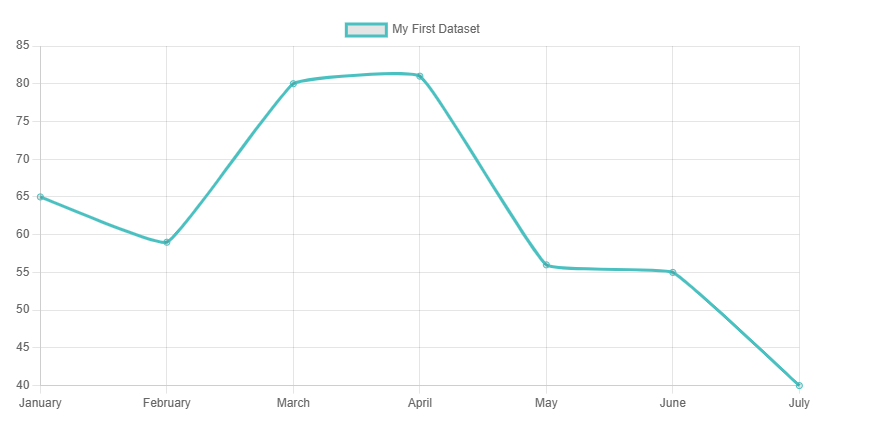
\includegraphics[width=0.8\linewidth]{gambar/Dasar teori/LineChart.png}
	\caption{Bentuk Line Chart}
	\label{gambar1}
\end{figure}

\subsubsection{Bar Chart}
Bar Chart adalah metode untuk menampilkan nilai data dalam bentuk batang vertikal. Grafik ini seringkali digunakan untuk menunjukkan tren data serta membandingkan beberapa set data secara berdampingan [25].

\begin{figure}[H]
	\centering
	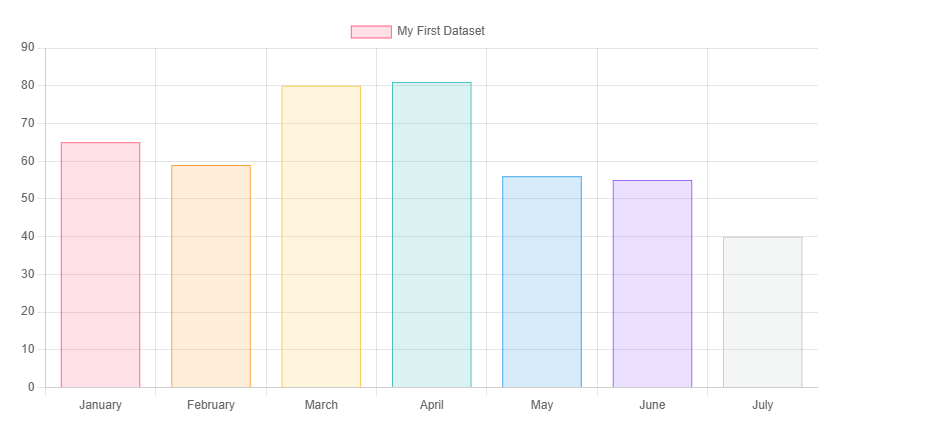
\includegraphics[width=0.8\linewidth]{gambar/Dasar teori/Bar Chart.png}
	\caption{Bentuk Bar Chart}
	\label{gambar1}
\end{figure}

\subsubsection{Scatter Plot}
Scatter plot merupakan salah satu jenis grafik yang membandingkan nilai data numerik dari dua variabel menggunakan titik yang berada dalam koordinat (x,y). Biasanya, jenis grafik ini digunakan untuk membandingkan nilai antar variabel [25]

\begin{figure}[H]
	\centering
	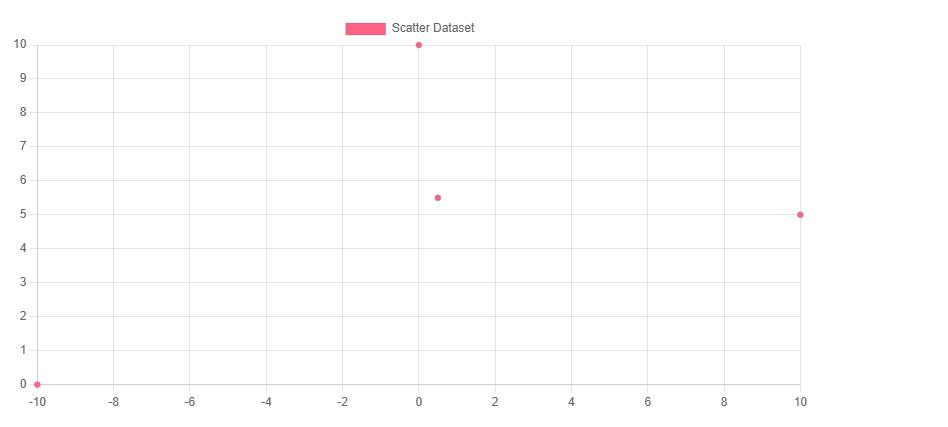
\includegraphics[width=0.8\linewidth]{gambar/Dasar teori/scatter.png}
	\caption{Bentuk Scatter Plot}
	\label{gambar1}
\end{figure}

\subsection{IoT}
Internet of Things (IoT) adalah konsep yang bertujuan untuk memperluas manfaat konektivitas internet yang selalu terhubung. IoT mengacu pada sistem di mana berbagai objek di dunia nyata dapat saling berkomunikasi dalam sebuah jaringan yang terintegrasi dengan internet sebagai perantara utamanya. Secara umum, cara kerja IoT berlandaskan pada tiga elemen utama, yaitu perangkat fisik yang telah dilengkapi modul IoT, perangkat koneksi seperti modem dan router nirkabel untuk menghubungkan ke internet, serta pusat data berbasis cloud yang berfungsi sebagai tempat penyimpanan aplikasi dan basis data. Modul IoT ini akan mengumpulkan serta mengirimkan data dalam rentang waktu tertentu sesuai dengan konfigurasi yang telah ditetapkan [27].

\subsection{Dataset}
Secara umum, dataset didefinisikan sebagai kumpulan data yang dikumpulkan dan disusun dalam suatu format tertentu untuk digunakan dalam analisis lebih lanjut. Definisi dataset didefinisikan sesuai konteks penggunaannya, seperti dalam ilmu komputer, statistik, atau penelitian ilmiah \cite{Renear2010}. Pada konteks penelitian ini, dataset ini merupakan data yang dihasilkan secara terus menerus dari perangkat IoT. Format data yang akan digunakan adalah JSON dan akan diuji cobakan sebagai data yang akan ditampilkan dalam visualisasi dan menentukan hasil evaluasi nantinya. 

\subsection{Pengujian Performa}
Performa mengacu pada proses evaluasi, pengukuran, dan penilaian terhadap efisiensi dalam menyelesaikan suatu tugas. Dalam bidang komputasi, performa menggambarkan efektivitas sebuah komputer dalam menjalankan suatu proses. Indikator utama dalam mengukur performa adalah jumlah waktu dan sumber daya yang digunakan untuk menyelesaikan tugas tersebut [28]. Dalam penelitian ini, performa yang diukur antara lain adalah rendering, scalability, dan penggunaan resource CPU dan memori. 

\subsubsection{Rendering}
Rendering merupakan proses pembuatan tampilan visual dalam bentuk gambar atau model 3D. Terdapat 2 jenis metode rendering yang dapat dilakukan, yaitu Hardware rendering dan Software Rendering. Software rendering memanfaatkan CPU untuk memproses dan menampilkan gambar, sementara hardware rendering menggunakan GPU untuk mempercepat proses tersebut [29].

\subsubsection{Scalability}
Konsep ini menggambarkan kemampuan suatu sistem untuk beradaptasi dengan pertambahan elemen atau objek, menangani peningkatan beban kerja secara efisien, serta dapat diperluas sesuai kebutuhan. Dalam proses perancangan sistem, skalabilitas sering menjadi faktor utama yang harus dipenuhi [30].

\subsubsection{CPU}
Berbeda dari implementasi perangkat keras lainnya, CPU merupakan perangkat yang sangat fleksibel karena dapat diprogram melalui perangkat lunak. CPU dianggap sebagai komponen dengan konsumsi energi terbesar dalam sebuah komputer. Oleh karena itu, dalam setiap penelitian, pengukuran penggunaan CPU selalu diperhitungkan untuk memperkirakan energi yang digunakan hanya oleh sebuah program computer. Pengukuran penggunaan CPU dapat ditinjau melalui Task Manager atau dengan skrip yang dibuat melalui terminal [31].

\subsubsection{Footprint Memory}
Footprint memory adalah total jumlah memori yang digunakan oleh suatu program, aplikasi, atau proses pada saat berjalan (runtime). Memory footprint digunakan untuk menggambarkan konsumsi memori dari sebuah aplikasi terhadap sistem komputer. Komponen memory footprint meliputi:
\begin{enumerate}
	\item Private memory yang digunakan hanya pada tab spesifik 
	\item Heap memory yang menyimpan objek dan struktur data dinamis.
	\item Stack memory yang digunakan untuk menyimpan variabel lokal dan kontrol eksekusi fungsi.
	\item Buffer dan cache internal yang menyimpan data sementara dari tab website.
\end{enumerate}

\subsubsection{Scalability}
Konsep ini menggambarkan kemampuan suatu sistem untuk beradaptasi dengan pertambahan elemen atau objek, menangani peningkatan beban kerja secara efisien, serta dapat diperluas sesuai kebutuhan. Dalam proses perancangan sistem, skalabilitas sering menjadi faktor utama yang harus dipenuhi [30].

\subsection{Random Access Memory(RAM)}
Memori adalah komponen dalam komputer yang berfungsi untuk menyimpan program dan data. Memori memiliki berbagai jenis, teknologi, struktur, dan kinerja yang bervariasi, tergantung pada cara informasi disimpan, dibaca, dan ditulis. CPU memiliki tiga tingkat cache, yang juga dikenal sebagai RAM internal. RAM internal membantu meningkatkan kinerja prosesor yang memungkinkan instruksi dikirim ke CPU lebih cepat dibandingkan jika diambil dari RAM eksternal. Saat CPU membutuhkan data, pencarian pertama dilakukan di cache Level 1 (L1), kemudian di Level 2 (L2), dan terakhir di Level 3 (L3). Jika data tidak ditemukan dalam cache, CPU akan mengambilnya dari DRAM [32]. Salah satu bagian dari RAM yang digunakan untuk memproses alokasi memori dinamis adalah heap memory. Heap memory akan menunjukkan distribusi memori di antara objek JavaScript pada halaman dan node DOM terkait. Penggunaan RAM ini dapat dipantau pada komputer, salah satunya melalui Chrome Task Manager pada kolom memory footprint. 

\subsection{Chrome Task Manager}
Task Manager merupakan ekstensi Chrome yang dapat digunakan untuk memantau dan mengelola berbagai proses yang berjalan di dalam browser.  Beberapa hal yang diukur dan ditampilkan oleh Chrome Task Manager antara lain:
\begin{enumerate}
	\item Penggunaan CPU menunjukkan seberapa banyak prosesor yang digunakan oleh setiap proses. 
	\item Memory Footprint mengukur jumlah memori yang digunakan oleh setiap proses, termasuk tab, ekstensi, dan plugin. Hal ini membantu dalam mengidentifikasi proses yang memakan banyak RAM.
	\item Network memantau aktivitas jaringan dari setiap proses sehingga penggunaan bandwith dapat terpantau. 
	\item Process ID merupakan id yang dapat digunakan untuk pelacakan dan diagnostik lebih lanjut.
\end{enumerate}
\chapter[METODOLOGI PENELITIAN]{\\ METODOLOGI PENELITIAN}
\section{Bahan}
Dalam proses penelitian, diperlukan data yang akan digunakan sebagai bahan pengujian untuk mengukur dan mengevaluasi kinerja metode yang diterapkan. Bahan uji yang digunakan merupakan data dummy yang dirancang dengan struktur menyerupai dataset asli yang diperoleh dari perangkat sensor IoT. Meskipun bukan data asli, dataset ini tetap mempertahankan variabel dan pola data yang umumnya ditemukan pada sensor IoT. Dengan menggunakan dataset dummy, penelitian ini dapat mensimulasikan kondisi real dari hasil sensor tanpa harus bergantung pada data aktual, sehingga memungkinkan pengujian yang lebih fleksibel dan berulang. Selain itu, pendekatan ini juga membantu dalam memahami bagaimana sistem bekerja dalam berbagai skenario yang mungkin terjadi pada sistem berbasis IoT, termasuk skenario yang sulit diperoleh dari data sensor asli. Pembuatan data IoT ini merujuk pada jurnal-jurnal yang membahas mengenai penggunaan sensor baik sebagai single-sensor maupun multiple-sensor. Penulis merancang data tersebut dalam format API yang mengacu pada penelitian yang dilakukan oleh Arief \cite{Triawan2023} serta Kasera dan Acharjee [33]. 

\begin{enumerate}[label={\alph*.}]
	\item Dummy Single Sensor BME380 \\
	Berdasarkan data yang diperoleh dari jurnal berjudul “Sistem Pemantauan Lingkungan Menggunakan Sensor BME280 Berbasis Internet of Things” \cite{Triawan2023} oleh Arief, struktur data dalam format JSON yang digunakan adalah sebagai berikut : 
	\pagebreak
	
	\begin{longtable}{|p{.35\linewidth}|p{.60\linewidth}|}
		\caption{Struktur JSON dari Sensor}
		\label{tab:json_sensor} \\  
		\hline
		\multicolumn{2}{|l|}{\textbf{Struktur JSON:}} \\ \hline
		\multicolumn{2}{|c|}{%
			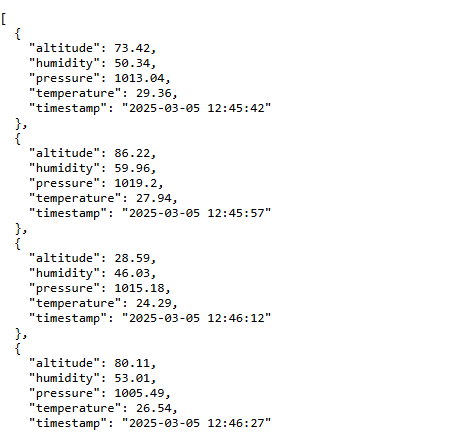
\includegraphics[width=0.8\linewidth, margin=5pt 10pt 5pt 10pt ]{gambar/Metodologi/StrukturJson.png}
		} \\ \hline
		\textbf{Parameter} & \textbf{Keterangan} \\ \hline
		\texttt{altitude} & Posisi vertikal (ketinggian) suatu objek dari suatu titik tertentu (datum). Dalam hal ini adalah mdpl. \\ \hline
		\texttt{humidity} & Kelembaban yang ditangkap dari sensor. \\ \hline
		\texttt{pressure} & Tekanan udara yang ditangkap dari sensor. \\ \hline
		\texttt{temperature} & Suhu yang ditangkap dari sensor. \\ \hline
		\texttt{timestamp} & Waktu saat data ter-generate. \\ \hline
	\end{longtable}
	
	Pada implementasinya, data dari referensi asli diolah menggunakan bahasa pemrograman Python hingga data menjadi API dalam format JSON. Tahapan pengolahan data dummy tersebut dijelaskan sebagai berikut : \\
	\begin{enumerate}[label={\arabic*.}]
		\item Mengidentifikasi jenis sensor yang akan digunakan. Dalam hal ini, sensor tersebut adalah sensor BME280. Sensor ini merupakan modul sensor yang dapat mengukur kelembaban, suhu, tekanan barometrik, dan ketinggian. Pada penerapannya, sensor ini dapat digunakan dalam banyak lini, beberapa diantaranya adalah pertanian, perkebunan, dan penerapan lainnya yang berhubungan dengan cuaca. Suryana dalam penelitiannya menjelaskan sensor BME280 mudah digunakan karena tidak memerlukan komponen tambahan lain dan telah memiliki fitur pre-calibrated [34].
		\begin{figure}[H]
			\centering
			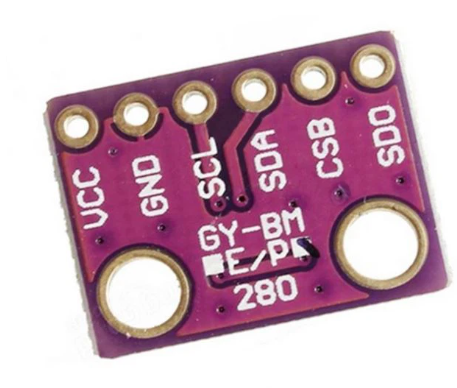
\includegraphics[width=0.8\linewidth]{gambar/Dasar teori/Sensor BME280.png}
			\caption{Sensor BME280}
			\label{gambar1}
		\end{figure}
		
		\item Menentukan rentang nilai yang akan dijadikan data dummy dengan merujuk pada penelitian yang membahas mengenai implementasi sensor BME280 pada studi kasus pengukuran stasiun cuaca dalam 3 hari berturut-turut. Mengacu pada penelitian tersebut, rentang data yang dihasilkan sensor dalam 10 detik berkisar sekitar 28,47℃ - 34,46 ℃ untuk suhu, 50,78\% - 59,17\% untuk kelembaban, 1008,27 hPa - 1009,24 hPa untuk tekanan udara, dan 40,14 - 63,67 m untuk ketinggian \cite{Triawan2023}. 
		
		\item Membuat file berformat Python dengan nama sensor-data.py.
		\item Menginstal Flask dengan perintah “pip install flask-cors”. Flask merupakan salah satu framework Python yang ringan dan mudah dikustomisasi serta dapat dimanfaatkan dalam pengembangan website. Flask menyediakan fitur yang dapat disesuaikan dengan kebutuhan pengembang tanpa harus berpatokan dengan standar atau struktur sebuah framework [35]. Pada konteks ini, Flask dimanfaatkan sebagai framework untuk pembuatan data API dummy yang akan digunakan untuk pengujian. Alasan pemilihan framework ini adalah karena ukurannya yang kecil dan fleksibilitasnya sehingga tidak membebani memori serta dapat dikonfigurasi dengan mudah. 
		\begin{figure}[H]
			\centering
			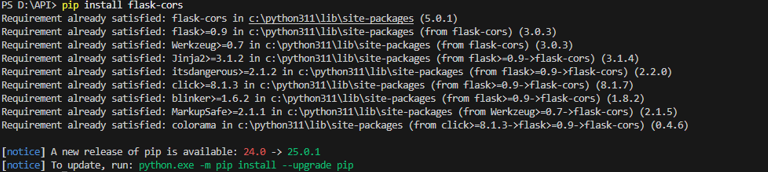
\includegraphics[width=0.8\linewidth]{gambar/Dasar teori/Flask.png}
			\caption{Install Flask}
			\label{Instal Flask}
		\end{figure}
		
		\item Menerapkan beberapa library, seperti berikut : 
		\begin{figure}[H]
			\centering
			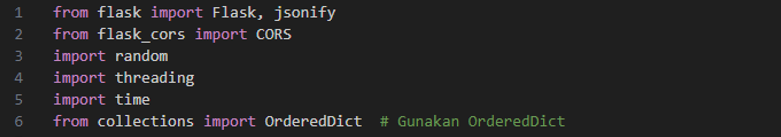
\includegraphics[width=0.8\linewidth]{gambar/Dasar teori/Library.png}
			\caption{Library}
			\label{Menambahkan Library}
		\end{figure}
		\begin{enumerate}[label={\alph*.}]
			\item jsonify: Mengubah data menjadi format JSON untuk dikirim ke client.
			\item CORS: Mengizinkan permintaan dari domain berbeda (Cross-Origin Resource Sharing). Digunakan untuk menghubungkan port 5000 dari python dan port 8000 dari HTTP. 
			\item random: Digunakan untuk menghasilkan data acak untuk membuat simulasi sensor. 
			\item threading: Digunakan untuk menjalankan fungsi secara paralel memperbarui data sensor secara terus-menerus.
			\item time: Mengatur delay dalam proses pembaruan data.
		\end{enumerate}
		
		\item Inisialisasi Flask dan Konfigurasi CORS
		\begin{figure}[H]
			\centering
			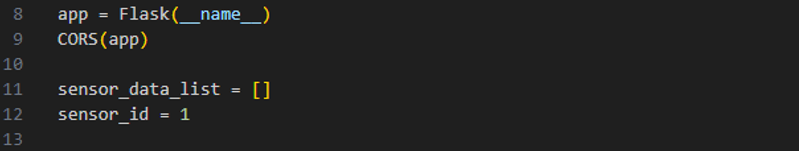
\includegraphics[width=0.8\linewidth]{gambar/Dasar teori/Initiate.png}
			\caption{Inisialisasi Flask dan CORS}
			\label{Inisialisasi Flask dan CORS}
		\end{figure}
		
		\item Variabel sensor\_data\_list digunakan untuk menyimpan data sensor yang terus diperbarui.
		\begin{figure}[H]
			\centering
			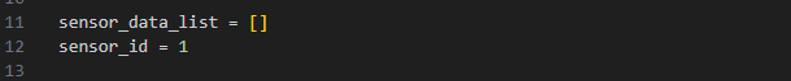
\includegraphics[width=0.8\linewidth]{gambar/Dasar teori/variabel.png}
			\caption{variabel}
			\label{Inisialisasi Variabel}
		\end{figure}
		
		\item Membuat fungsi untuk membuat data sensor yang menghasilkan dan menyimpan data setiap 10 detik dalam rentang data 28.47℃ - 34.53℃ untuk suhu, 59.13\% - 50.78\% untuk humidity, 1008 hPa - 1011 hPa untuk pressure, dan 40.16 m - 63.67m untuk altitude. Sensor ini dibuat untuk terus me-looping pembuatan data dengan struktur: 
		\begin{enumerate}[label={\alph*.}]
			\item Id nilai unik untuk mengidentifikasi data 
			\item Timestamp dalam format standar ISO 8601
			\item Temperature dalam satuan derajat celcius hingga derajat celcius 
			\item Humidity dalam satuan RH
			\item Pressure dalam satuan HPa 
			\item Altitude dalam satuan meter
		\end{enumerate}
		\begin{figure}[H]
			\centering
			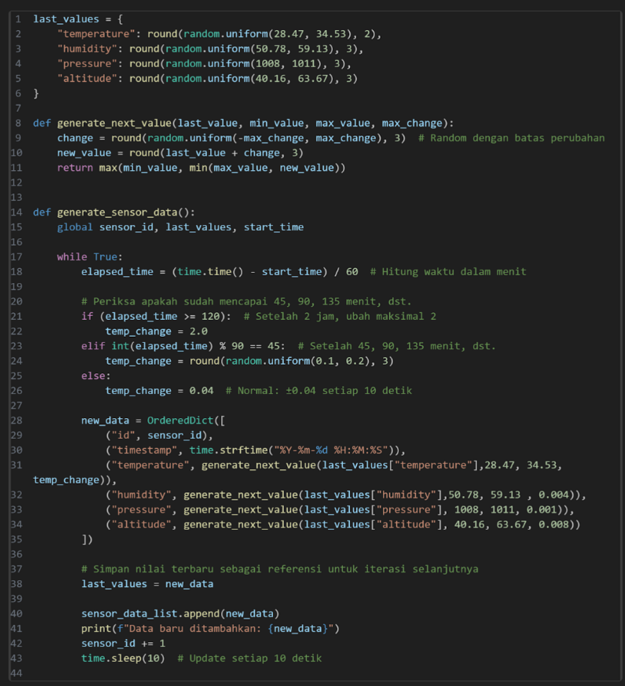
\includegraphics[width=0.8\linewidth]{gambar/Dasar teori/generate_dummy.png}
			\caption{Membuat Sensor Dummy}
			\label{Membuat Sensor Dummy}
		\end{figure}
		
		\item Membuat API Endpoint. API endpoint ini akan digunakan untuk mengambil data dan mengurutkannya dalam format JSON dengan library jsonify.
		\begin{figure}[H]
			\centering
			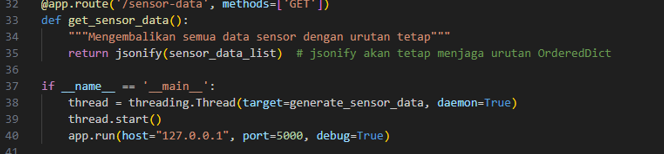
\includegraphics[width=0.8\linewidth]{gambar/Dasar teori/API.png}
			\caption{API Endpoint}
			\label{API Endpoint}
		\end{figure}
		
		\item Menjalankan program threading pada fungsi generate\_sensor\_data secara berkala, paralel dengan server Flask untuk menangani request.
		\begin{figure}[H]
			\centering
			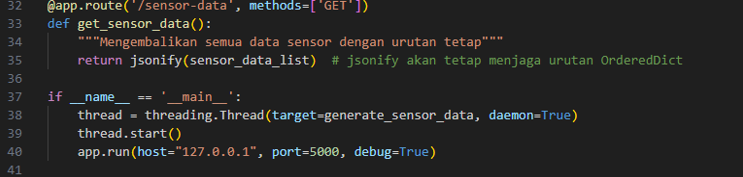
\includegraphics[width=0.8\linewidth]{gambar/Dasar teori/threading.png}
			\caption{Menjalankan Program Threading}
			\label{Menjalankan Program Threading}
		\end{figure} 
		
		\item Menjalankan server tersebut dengan “python sensor-data.py”. 
		\begin{figure}[H]
			\centering
			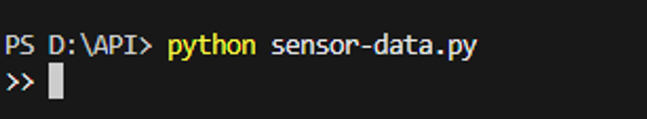
\includegraphics[width=0.8\linewidth]{gambar/Dasar teori/Run.png}
			\caption{Menjalankan Sensor}
			\label{Menjalankan Sensor}
		\end{figure}
	\end{enumerate}
	\item Multiple Sensor \\
	Data yang dijadikan acuan sebagai contoh data yang mengintegrasikan beberapa sensor pengukuran adalah data yang merujuk pada jurnal “A Comprehensive IoT edge based smart irrigation system for tomato cultivation” [33]. Berdasarkan data yang diperoleh dari jurnal tersebut, struktur json yang ditampilkan adalah sebagai berikut :
	\pagebreak
	\begin{longtable}{|p{.35\linewidth}|p{.60\linewidth}|}
		\caption{Struktur JSON dari Sensor}
		\label{tab:json_sensor} \\  
		\hline
		\multicolumn{2}{|l|}{\textbf{Struktur JSON:}} \\ \hline
		\multicolumn{2}{|c|}{%
			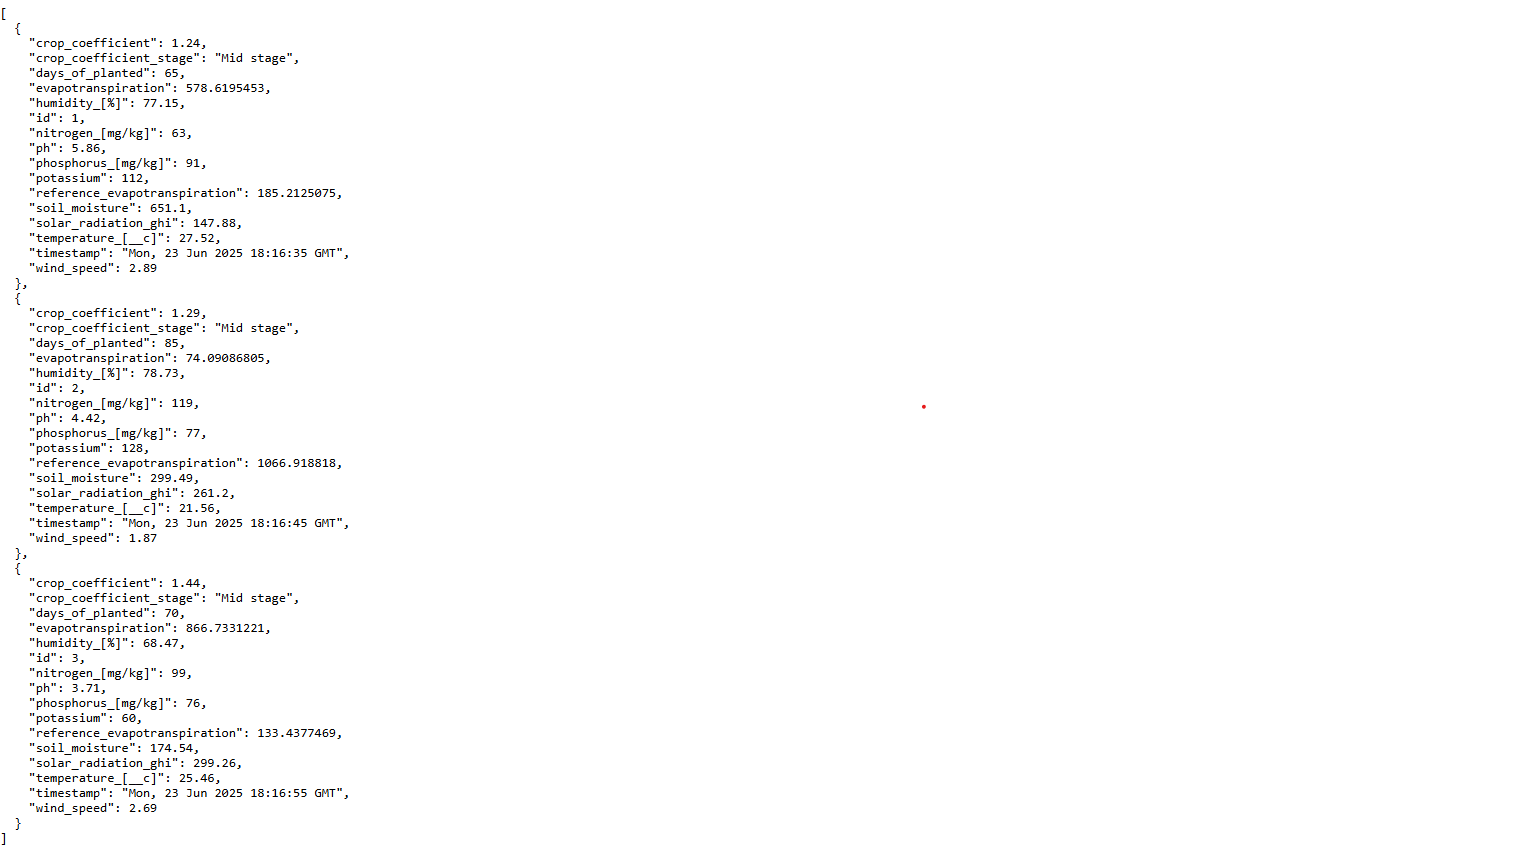
\includegraphics[width=0.8\linewidth, margin=5pt 10pt 5pt 10pt ]{gambar/Metodologi/StrukturJSON2.png}
		} \\ \hline
		\textbf{Parameter} & \textbf{Keterangan} \\ \hline
		\texttt{crop\_coefficient} & Koefisien tanaman (Kc) menggambarkan kebutuhan air relatif tanaman pada fase pertumbuhan tertentu \\ \hline
		\texttt{crop\_coefficient\_stage} & Tahapan pertumbuhan tanaman saat ini \\ \hline
		\texttt{days\_of\_planted} & Hari sejak tanaman ditanam \\ \hline
		\texttt{evapotranspitarion} & Jumlah air yang hilang akibat penguapan \\ \hline
		\texttt{humidity} & Kelembapan udara \\ \hline
		\texttt{nitrogen} & Kandungan nitrogen pada tanah \\ \hline
		\texttt{ph} & Tingkat keasaman tanah \\ \hline
		\texttt{phosphorus} & Kandungan fosfor pada tanah \\ \hline
		\texttt{potassium} & Kandungan kalium di dalam tanah \\ \hline
		\texttt{reference\_evaporation} & nilai standar berdasarkan tanaman acuan\\ \hline
		\texttt{soil\_mosture} & kelembapan tanah \\ \hline
		\texttt{solar\_radiation\_ghi} & Radiasi\\ \hline
		\texttt{temperature} & Suhu udara saat pengukuran \\ \hline
		\texttt{timestamp} & Waktu saat data diambil \\ \hline
		\texttt{windspeed} & Kecepatan angin \\ \hline
	\end{longtable}
	Tahapan yang dilakukan dalam menampilkan data tersebut menjadi data real-time yang siap uji antara lain : 
	\begin{enumerate}[label={\arabic*.}]
		\item Mengunduh sumber data hasil pengukuran dalam bentuk csv. 
		\item Memanfaatkan framework Flask untuk menampilkan data tersebut dan menggunakan library pandas untuk mengolah data csv.
		\item Melakukan data preprocessing dengan mengubah semua huruf menjadi huruf kecil, mengganti spasi dengan underscore agar mudah dipahami, serta melakukan teknik oversampling pada data agar data bertambah dari jumlah data aslinya. Teknik oversampling adalah teknik untuk menambahkan data dari kelas minoritas ke dalam data pelatihan secara acak. Penambahan ini dilakukan berulang-ulang hingga jumlah data pada kelas minoritas setara dengan jumlah data pada kelas mayoritas [36]
		\begin{figure}[H]
			\centering
			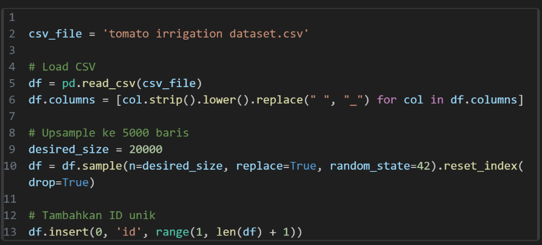
\includegraphics[width=0.8\linewidth]{gambar/Metodologi/Mount_preprocessing.png}
			\caption{Mounting Data}
			\label{Mounting Data}
		\end{figure}
		\item Membuat kolom timestamp agar dapat menampilkan data secara realtime selama pengujian. 
		\begin{figure}[H]
	\centering
	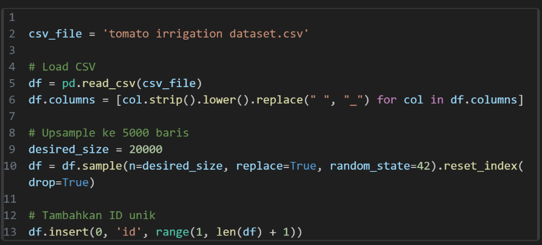
\includegraphics[width=0.8\linewidth]{gambar/Metodologi/kolom_timestamp.png}
	\caption{Membuat kolom timestamp}
	\label{Membuat Timestamp Data}
\end{figure}
		\item Membuat endpoint untuk mengambil data sensor dan menambahkan data ke dalam json setiap 10 detik. Data akan terus menerus digenerate seperti ketika sensor mengambil data real-time dari aplikasi. 
		\begin{figure}[H]
			\centering
			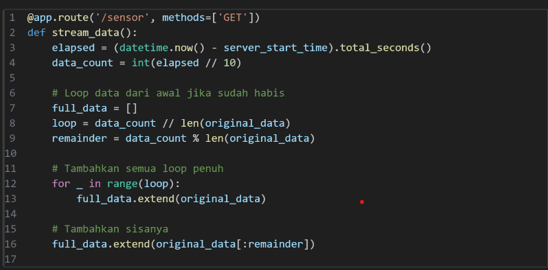
\includegraphics[width=0.8\linewidth]{gambar/Metodologi/endpoint.png}
			\caption{Membuat Endpoint API}
			\label{Membuat Endpoint}
		\end{figure}
		\item Menjalankan server Flask dalam mode debug untuk mempermudah pengembangan karena auto-reload dan error ditampilkan.
		\begin{figure}[H]
			\centering
			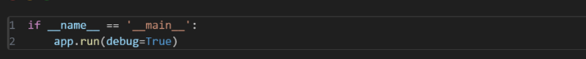
\includegraphics[width=0.8\linewidth]{gambar/Metodologi/run.png}
			\caption{Menjalankan Server}
			\label{Menjalankan Server}
		\end{figure}
		
	\end{enumerate}
\end{enumerate}

\section{Alat}
Salah satu tujuan penelitian ini adalah untuk meninjau performa rendering dan penggunaan resource pada perangkat saat melakukan visualisasi data dari perangkat sensor IoT. Oleh karena itu, penelitian ini membutuhkan peralatan software dan hardware untuk menunjang penelitian.
\subsection{Perangkat Lunak}
Peralatan perangkat lunak yang digunakan dalam pengembangan sistem ini, meliputi sistem operasi, library, dan aplikasi yang digunakan, yang dijelaskan sebagai berikut :  

\begin{longtable}{|p{\dimexpr.35\linewidth-2\tabcolsep-1.25\arrayrulewidth}|
		p{\dimexpr.20\linewidth-2\tabcolsep-1.25\arrayrulewidth}|
		p{\dimexpr.45\linewidth-2\tabcolsep-1.25\arrayrulewidth}|}
	\caption{Spesifikasi Perangkat Lunak} \label{t_risetPemodelan} \\
	
	\hline
	\textbf{Nama Perangkat Lunak} & \textbf{\textit{Versi}} & \textbf{Keterangan} \\ \hline
	\endfirsthead
	
	\hline
	\textbf{Nama Perangkat Lunak} & \textbf{\textit{Versi}} & \textbf{Keterangan} \\ \hline
	\endhead
	
	\hline \multicolumn{3}{r}{{Lanjut ke halaman berikutnya}} \\ 
	\endfoot
	
	\hline
	\endlastfoot
	
	Visual Studio Code & 1.97.0 & Digunakan untuk membuat \textit{website}, dari segi \textit{Frontend} dan \textit{Backend}. \\ \hline
	
	Python & 3.11.4 & Digunakan untuk membuat data \textit{dummy} guna menguji cobakan \textit{chart} visualisasi. \\ \hline
	
	Chart.js & 4.0 & \textit{Versi} Chart.js saat diuji cobakan. Digunakan untuk membuat visualisasi. \\ \hline
	
	D3.js & 7.9.0 & \textit{Versi} D3.js saat diuji cobakan. Digunakan untuk membuat visualisasi. \\ \hline
	
	Highcharts & 12.1.2 & \textit{Versi} Highcharts saat diuji cobakan. Digunakan untuk membuat visualisasi. \\ \hline
	
\end{longtable}


\subsection{Perangkat Keras}
Peralatan perangkat keras yang digunakan dalam pengembangan sistem ini, meliputi spesifikasi laptop yang digunakan untuk mengembangkan dan menjalankan website, yang dijelaskan sebagai berikut :  

\begin{table}[h!]
	\centering
	\renewcommand{\arraystretch}{1.5} % jarak baris lebih renggang
	\caption{\textit{Spesifikasi Perangkat Keras yang Digunakan}}
	\label{tab:spesifikasi_perangkat_keras}
	\begin{tabular}{|>{\raggedright\arraybackslash}p{4cm} 
			|>{\raggedright\arraybackslash}p{8cm}|}
		\hline
		\textbf{Spesifikasi} & \textbf{Keterangan} \\
		\hline
		Operating System & Windows 11 64-bit \\
		\hline
		Processor & Intel(R) Core (TM) i5-10300H \\
		\hline
		CPU & 2.5 GHz \\
		\hline
		Memory & 8GB DDR4 SO-DIMM 2666MHz \\
		\hline
		Graphic & NVIDIA\textregistered~GeForce\textregistered~GTX 1650 4GB GDDR6 \\
		\hline
	\end{tabular}
\end{table}


\section{Tahapan Proyek Akhir}
Dalam penelitian yang berjudul Analisis Perbandingan Kinerja Library Chart.js, Highcharts, dan D3.js untuk Visualisasi Data Sensor IoT pada Dashboard Berbasis Laravel, penulis melalui beberapa tahapan penting untuk mendapatkan hasil yang komprehensif. Tahapan pertama adalah fase studi literatur, selanjutnya adalah pengembangan website, di mana penulis membangun sebuah dashboard berbasis Laravel yang mampu menampilkan data sensor IoT secara dinamis. Setelah itu, pada fase implementasi library, tiga library visualisasi Chart.js, Highcharts, dan D3.js diimplementasikan ke dalam sistem untuk menampilkan data dalam format grafik line chart. Tahapan terakhir adalah fase komparasi, yang bertujuan untuk mengevaluasi kinerja masing-masing library berdasarkan berbagai parameter yang telah ditentukan sebelumnya. Melalui pendekatan ini, penelitian diharapkan dapat memberikan wawasan mendalam mengenai library yang paling optimal untuk memvisualisasikan data IoT. Alur penelitian ini dijelaskan dalam bagan berikut : 

\begin{figure}[H]
	\centering
	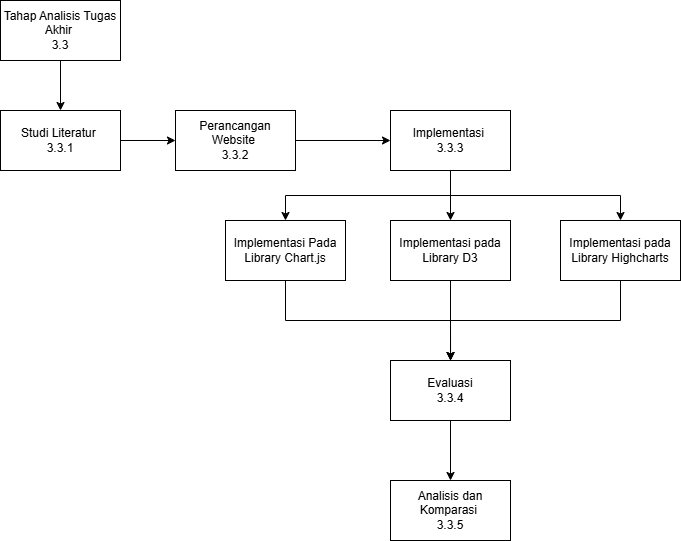
\includegraphics[width=0.8\linewidth]{gambar/Metodologi/Alur penelitian.png}
	\caption{Alur Penelitian}
	\label{Alur Penelitian}
\end{figure}

\subsection{Studi Literatur}
Tahap ini dilakukan untuk memperoleh landasan yang mendukung pelaksanaan penelitian. Literatur yang dikaji mencakup teori-teori utama yang relevan dengan topik, serta penelitian terdahulu yang berkaitan dengan pendekatan dan metode yang digunakan dalam penelitian ini. 

Penelitian dilakukan dengan menggunakan metode eksperimen dengan pendekatan kuantitatif. Pendekatan ini dilakukan secara runtut dan rasional, di mana peneliti secara langsung mengatur variabel bebas untuk melihat dampaknya terhadap variabel yang dipengaruhi, dalam situasi yang telah dikendalikan. Dengan metode ini, peneliti memiliki kontrol atas variabel bebas baik sebelum maupun saat proses eksperimen berlangsung. Proses ini juga disertai dengan pengukuran data secara kuantitatif guna mengetahui adanya hubungan sebab dan akibat antara variabel yang diteliti. Tujuan dari pendekatan ini adalah untuk menguji kebenaran hipotesis yang telah dirumuskan, memperkirakan hasil dari perlakuan yang diberikan, serta menyimpulkan pola hubungan antar variabel secara umum [37]. Dalam konteks ini, variabel bebas yang dimaksud adalah Chart.js, D3, dan Highcharts, serta variabel terikat adalah waktu render, penggunaan CPU, dan penggunaan memori.

Terdapat beberapa studi literatur yang digunakan sebagai acuan pengukuran dalam penelitian ini. Berdasarkan rujukan jurnal yang dijelaskan pada bab sebelumnya, waktu rendering, penggunaan memori, dan alokasi CPU seringkali dijadikan sebagai indikator pengukuran performa suatu website visualisasi karena ketiganya memengaruhi alokasi sumber daya (resources) pada sistem komputer yang menentukan pengalaman pengguna (user experience) dan efisiensi sistem \cite{Persson2021} \cite{Persson2021}, [35].

Berdasarkan rujukan yang digunakan, indikator tersebut berbanding lurus dan saling mempengaruhi satu sama lain. Peningkatan pada satu indikator cenderung diikuti oleh peningkatan pada indikator lainnya. Misalnya, karena kompleksitas visualisasi yang tinggi atau penggunaan fitur interaktif yang intensif, maka penggunaan memori juga akan bertambah untuk menyimpan elemen visual serta data yang ditampilkan. Korelasi ini menjadi penting untuk dianalisis secara menyeluruh guna memahami performa sistem secara holistik. Fitur-fitur utama dari visualisasi data seperti interaktivitas, kompleksitas elemen grafik, jumlah data yang divisualisasikan, serta kemampuan dukungan real-time sangat memengaruhi performa render. Semakin tinggi tingkat interaktivitas serta semakin kompleks grafik, maka semakin besar pula beban terhadap CPU dan memori sistem, serta semakin lama waktu yang dibutuhkan untuk menampilkan visualisasi secara utuh. Merujuk pada website dari Chart.js [5], D3.js [6], dan Highcharts [7], perbandingan yang ditinjau dari aspek yang telah disebutkan dijelaskan seperti pada tabel berikut :
\begin{table}[H]
	\centering
	\renewcommand{\arraystretch}{1.5} % jarak baris lebih renggang
	\caption{Perbandingan Chart.js, D3.js, dan Highcharts}
	\label{tab:perbandingan_library}
	\begin{tabular}{|>{\raggedright\arraybackslash}p{3.5cm}
			|>{\raggedright\arraybackslash}p{3.5cm}
			|>{\raggedright\arraybackslash}p{3.5cm}
			|>{\raggedright\arraybackslash}p{3.5cm}|}
		\hline
		\rowcolor[gray]{0.85}
		\textbf{Aspek} & \textbf{Chart.js} & \textbf{D3.js} & \textbf{Highcharts} \\
		\hline
		Ketersediaan \textit{open source} 
		& Tersedia 
		& Tersedia 
		& Tersedia \\ 
		\hline
		Dukungan Interaktif 
		& Mendukung interaktivitas seperti \textit{tooltip}, \textit{zoom}, dan \textit{hover}. 
		& Interaksi kompleks termasuk \textit{tooltip}, \textit{zoom}, dan animasi.
		& Interaktif dengan built-in fitur \textit{tooltip}, \textit{drilldown}, \textit{zoom}, \textit{pan}, dan animasi. \\
		\hline
		Basis grafik 
		& Menggunakan Canvas 
		& Menggunakan SVG atau Canvas 
		& Menggunakan SVG (default) \\
		\hline
		Dukungan data \textit{real-time} 
		& Didukung dengan update dinamis menggunakan \texttt{chart.update()} 
		& Harus dikodekan manual 
		& Mendukung data \textit{real-time} dengan fitur bawaan \texttt{setData()} \\
		\hline
	\end{tabular}
\end{table}

\subsection{Perancangan Website}
Dalam prosesnya, pengembangan website ini dibagi menjadi dua bagian utama, yaitu Frontend dan Backend. Frontend merupakan sisi pengembangan yang berfokus pada tampilan dan interaksi pengguna. Sementara Backend menangani manajemen database dan API. Penelitian ini secara khusus berfokus pada pengembangan Frontend yang mencakup implementasi desain serta analisis penggunaan Library visualisasi. Proses pengembangan Frontend melibatkan berbagai teknologi seperti HTML, CSS, dan JavaScript. Dengan fokus pada Frontend, penelitian ini bertujuan untuk menghasilkan tampilan website yang responsif dan mudah digunakan oleh pengguna. Adapun aspek Backend yang berhubungan dengan manajemen data dan logika pemrosesan tidak dibahas dalam penelitian ini, sehingga integrasi dengan sistem Backend akan menjadi pertimbangan dalam implementasi lanjutan.

\subsubsection{Perancangan Desain Sistem}
Selain data uji, diperlukan pula perancangan sistem yang menjadi bahan untuk mendefinisikan struktur, alur kerja, dan interaksi sistem sebelum tahap implementasi dilakukan. Pada tahap ini, diperlukan pendefinisian kebutuhan, use case diagram dan sequence diagram, serta kebutuhan data pengujian. Kebutuhan fungsional yang dimaksud mencakup fitur-fitur utama yang harus ada dalam sistem agar sesuai dengan tujuan. Berikut adalah beberapa kebutuhan fungsional dalam website yang menampilkan data IoT:

\begin{enumerate}[label={\arabic*.}]
	\item Website harus mampu mengambil data secara real-time melalui API.
	\item Website mampu menambahkan lebih dari satu visualisasi dengan dukungan terhadap jenis grafik seperti line chart, bar chart, dan scatter plot. 
\end{enumerate}

Sedangkan kebutuhan non-fungsional yang dimaksud, berkaitan dengan kualitas sistem dan aspek teknis yang memastikan website berjalan dengan optimal. Kebutuhan tersebut meliputi: 
\begin{enumerate}[label={\arabic*.}]
	\item Sistem mampu menangani volume data besar yang terus bertambah dari perangkat IoT.
	\item Kode terdokumentasi dengan baik, sehingga mudah diperbarui atau diperbaiki.
\end{enumerate}

Untuk mengimplementasi kebutuhan fungsional dan non fungsional, diagram yang dibutuhkan antara lain adalah use case diagram dan sequence diagram. Use Case Diagram adalah diagram Unified Modeling Language (UML) yang menggambarkan interaksi antara pengguna (actors) dengan sistem melalui berbagai fitur penggunaan (use cases). Use case diagram dapat membantu pengembang akan lebih mudah dalam melakukan analisis kebutuhan, serta merancang fitur yang akan dikembangkan. Pada sistem yang sedang diteliti, use case diagram berikut menggambarkan fitur-fitur yang berkaitan dengan penelitian, seperti gambar berikut :

\begin{figure}[H]
	\centering
	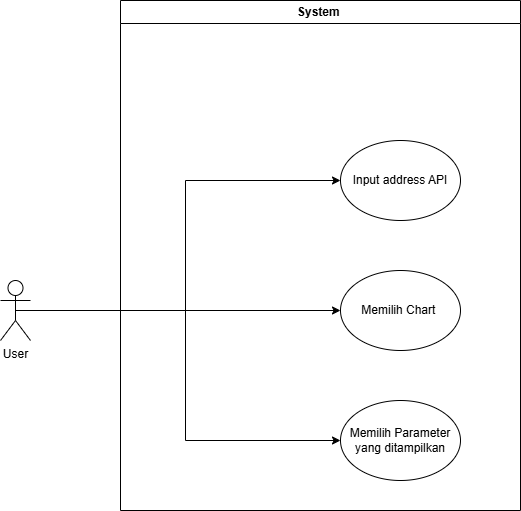
\includegraphics[width=0.8\linewidth]{gambar/Metodologi/Use Case.png}
	\caption{use Case Diagram}
	\label{Use Case Diagram}
\end{figure}

Sequence Diagram merupakan diagram UML yang digunakan untuk menggambarkan bagaimana objek berinteraksi dan bertukar pesan seiring waktu. Diagram ini menunjukkan bagaimana pesan dikirim antara objek atau instance lainnya untuk menyelesaikan suatu tugas. Sequence Diagram digunakan pada tahap perancangan detail, dimana komunikasi antar proses harus ditetapkan secara tepat [39].  Sequence Diagram untuk website ini digambarkan seperti berikut :

\begin{figure}[H]
	\centering
	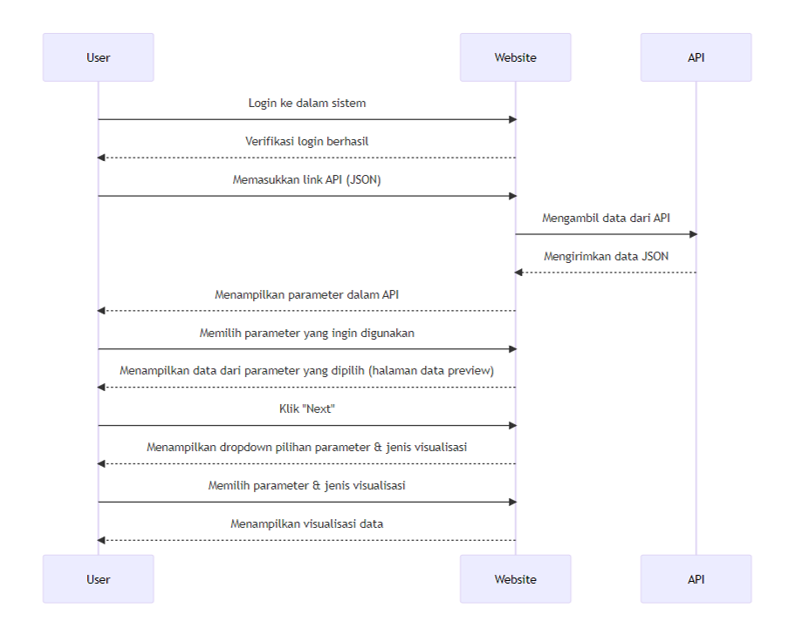
\includegraphics[width=0.8\linewidth]{gambar/Metodologi/Sequence Diagram.png}
	\caption{Sequence Diagram}
	\label{Sequence Diagram}
\end{figure}

\subsubsection{Perancangan UI}
Sebelum tahap pengembangan frontend, diperlukan perancangan User Interface dengan Figma yang akan digunakan sebagai acuan untuk membuat kode Frontend, rancangan user interface tersebut dibagi menjadi dua halaman utama dan 3 komponen tambahan, seperti berikut : 
\begin{enumerate}[label={\arabic*.}]
	\item Halaman Utama \\
	Halaman ini merupakan halaman pertama yang akan dilihat pengguna setelah mengakses website. Pada bagian ini, pengguna dapat menginputkan API dari data IoT pada field input yang tersedia, kemudian setelah di klik generate, parameter pada API tersebut akan tertampil dalam bentuk checkbox. 
	\begin{figure}[H]
		\centering
		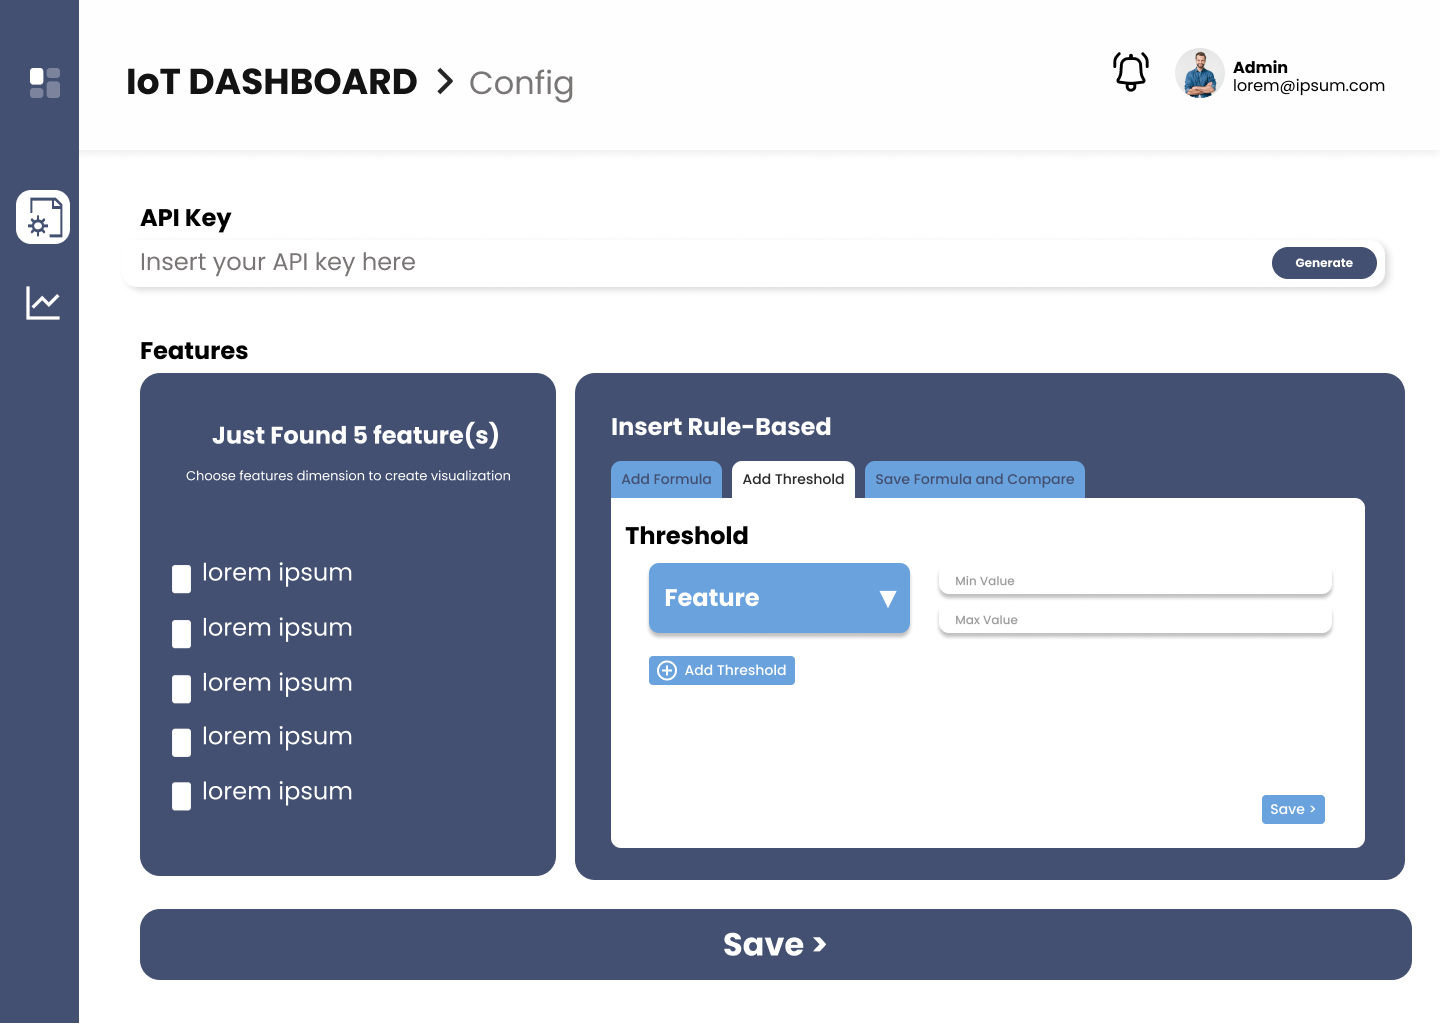
\includegraphics[width=0.8\linewidth]{gambar/Metodologi/main.png}
		\caption{Halaman Utama}
		\label{Halaman Utama}
	\end{figure}
	Adapun fitur yang ada di dalam halaman ini adalah kolom input alamat API untuk menginputkan alamat API dari pengguna, Checkbox untuk menampilkan parameter yang ada di dalam API, Tab rules untuk memberikan pengaturan terhadap data-data yang masuk. Seperti mengatur ambang batas, formula, dan komparasi formula. 
	\item Formula \\
	Merupakan fitur yang digunakan untuk menyimpan rumus tertentu yang dapat difungsikan sebagai threshold atau alert saat data menyentuh suatu titik tertentu yang dianggap tidak wajar. 
	\begin{figure}[H]
		\centering
		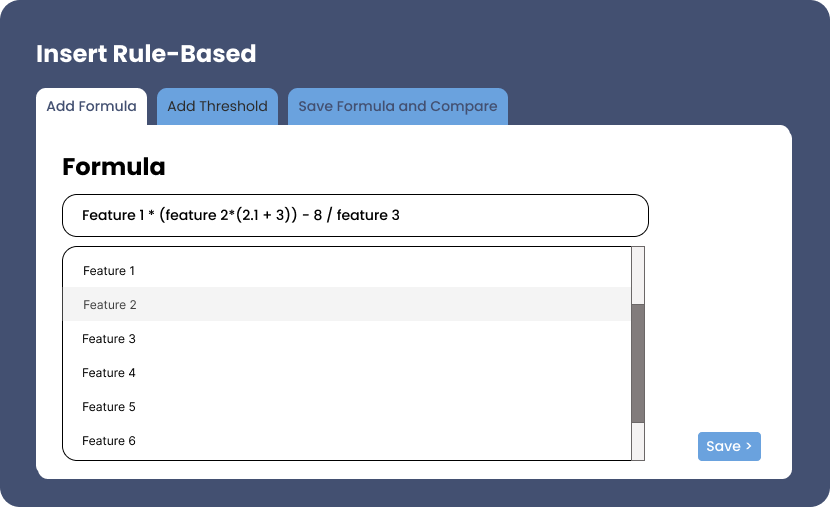
\includegraphics[width=0.8\linewidth]{gambar/Metodologi/formula.png}
		\caption{Menambahkan Formula}
		\label{gambar1}
	\end{figure}
	\item Threshold\\
	 Merupakan fitur yang digunakan untuk menyimpan ambang batas minimal dan maksimal dari suatu fitur data sehingga sistem akan memunculkan peringatan ketika data melampaui ambang batas. 
	 \begin{figure}[H]
	 	\centering
		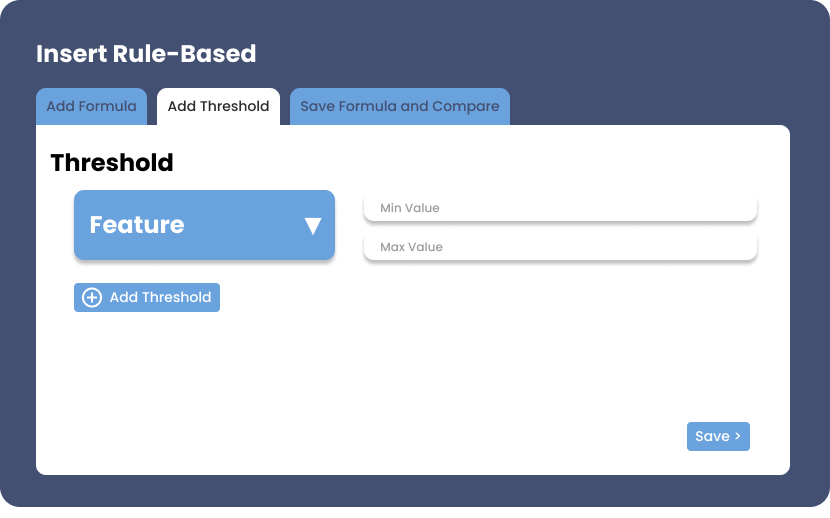
\includegraphics[width=0.8\linewidth]{gambar/Metodologi/threshold.png}
	 	\caption{Menambahkan Ambang Batas}
	 	\label{Menambahkan Ambang Batas}
	 \end{figure}
	 \item Save Formula and Compare\\
	 Digunakan untuk membandingkan antara threshold dan batasan tertentu. Sehingga ketika terdapat perbedaan, maka sistem akan menampilkan alert. Pada tab ini, pengguna dapat memilih dua fitur untuk dibandingkan. 
	 	 \begin{figure}[H]
	 	\centering
	 	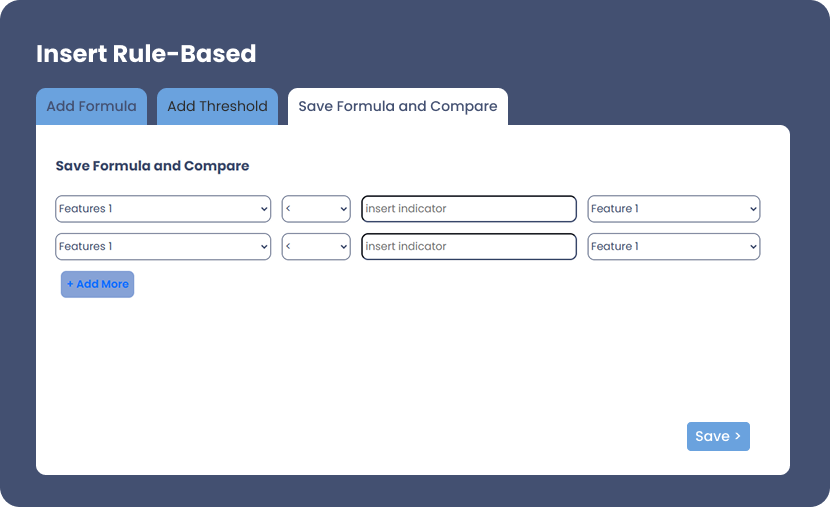
\includegraphics[width=0.8\linewidth]{gambar/Metodologi/compare.png}
	 	\caption{Menambahkan Ambang Batas}
	 	\label{Menambahkan Ambang Batas}
	 \end{figure}
	 \item Halaman visualisasi dan Chart\\
	 Halaman ini digunakan untuk memvisualisasikan perbandingan dari suatu fitur dengan fitur lainnya melalui bar chart, line chart, dan scatter plot.
	 	 \begin{figure}[H]
	 	\centering
	 	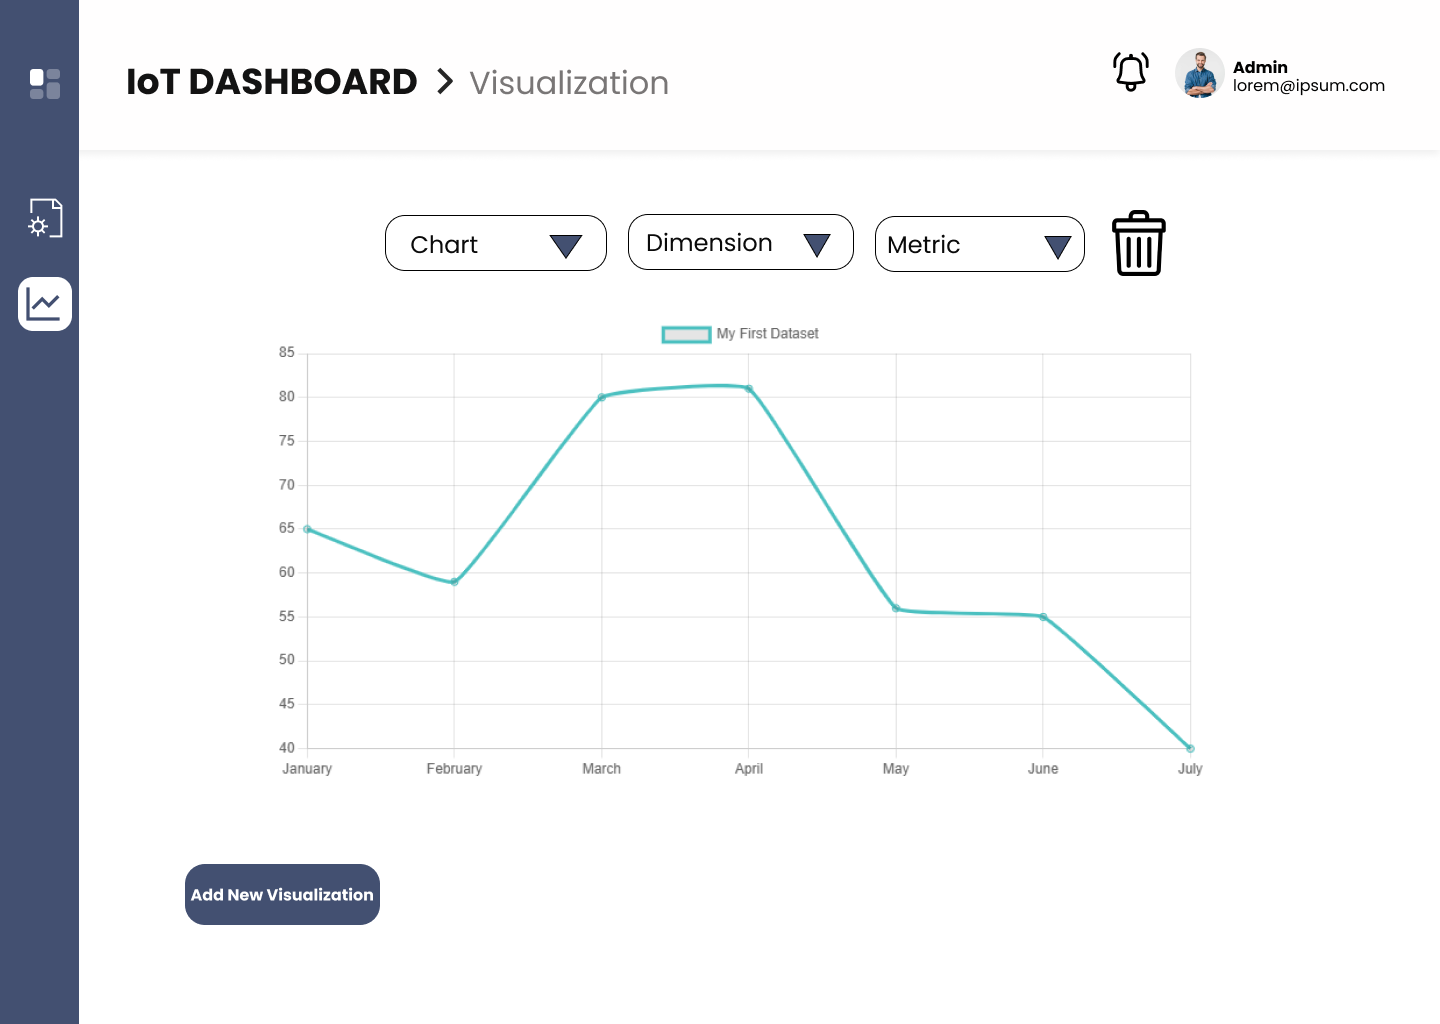
\includegraphics[width=0.8\linewidth]{gambar/Metodologi/visualization page.png}
	 	\caption{Menambahkan Ambang Batas}
	 	\label{Menambahkan Ambang Batas}
	 \end{figure} 
\end{enumerate}
\subsection{Implementasi}
Setelah menyiapkan data, maka tahap selanjutnya adalah tahap implementasi. Tahap ini akan menjelaskan implementasi Chart.js, D3.js, dan Highcharts dalam menampilkan visualisasi. Implementasi dilakukan dengan menggunakan skrip Javascript yang sama dengan penyesuaian pada bagian fungsi createChart() sesuai dengan library JavaScript yang digunakan. Fungsi-fungsi lain yang digunakan dalam tahap ini telah dijelaskan pada sub-bab “Pembuatan Website”. 

\subsection{Evaluasi}
Proses ini bertujuan untuk mengetahui perbedaan signifikan dalam waktu rendering, efisiensi pengolahan data visual, serta kemampuan masing-masing library dalam menangani beban visualisasi yang berbeda. Dalam prosesnya, semua pengujian dilakukan dalam lingkungan hardware, software, dan versi browser yang sama serta kondisi browser selalu dipastikan bersih sebelum melakukan pengujian lainnya dengan selalu memulai ulang kondisi browser. Dengan melakukan perbandingan ini, diharapkan dapat ditemukan library yang paling optimal dan sesuai untuk digunakan dalam pengembangan sistem visualisasi data. Setelah diimplementasikan, performa akan dievaluasi berdasarkan parameter-parameter yang telah ditentukan, meliputi : 
\begin{enumerate}
	\item Performa rendering

	Performa akan diukur dengan fungsi bawaan dari Javascript \cite{Persson2021} \cite{Persson2021}. Pengukuran dilakukan dengan memanfaatkan fungsi dari JavaScript console.time() dan performance.now() yang ditempatkan di dalam fungsi createChart() untuk mengukur waktu render. Fungsi performance.now() adalah fungsi di JavaScript yang digunakan untuk mengukur waktu secara presisi sehingga dapat digunakan untuk mengetahui durasi eksekusi suatu proses dalam aplikasi web [40]. Pengukuran ini dilakukan dengan tahapan : 
	\begin{enumerate}[label={\arabic*.}]
		\item menjalankan server data dummy dan server website secara lokal,
		\item menampilkan visualisasi pada website, 
		\item meninjau waktu render melalui file berformat .txt yang telah otomatis di-generate dari console menggunakan fungsi performance.now() yang memberikan nilai waktu relatif, yaitu berapa milidetik yang dihitung sejak fungsi dijalankan. 
			\begin{figure}[H]
			\centering
			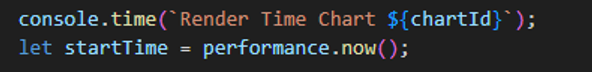
\includegraphics[width=0.8\linewidth]{gambar/Metodologi/Start Performance Now.png}
			\caption{Mulai Pengukuran}
			\label{Mulai Pengukuran Render}
		\end{figure}
			\begin{figure}[H]
			\centering
			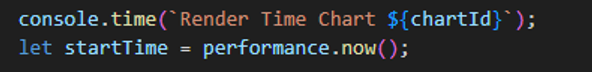
\includegraphics[width=0.8\linewidth]{gambar/Metodologi/Start Performance Now.png}
			\caption{Akhir Pengukuran}
			\label{Akhir Pengukuran Render}
		\end{figure}
	\end{enumerate}
			Setelah seluruh proses selesai dijalankan dan waktu render telah terekam, data tersebut akan digunakan untuk menghitung rata-rata waktu render di setiap titik yang telah ditentukan. Nilai rata-rata ini berperan penting dalam proses evaluasi, karena mampu mereduksi pengaruh noise atau outlier yang mungkin muncul selama pengujian. Dengan demikian, pengukuran performa website menjadi lebih stabil, representatif, dan dapat mencerminkan tingkat skalabilitas sistem secara lebih akurat.
	
	\item Alokasi Footprint Memory 
	
	Pengukuran penggunaan memori dilakukan dengan memanfaatkan fitur Chrome Task Manager, dengan cara mencatat nilai Memory Footprint pada tab Chrome tertentu. Nilai ini menggambarkan total memori yang digunakan oleh tab tersebut, mencakup memori yang dipakai untuk proses rendering halaman, eksekusi skrip JavaScript, serta pemuatan berbagai sumber daya yang ada di dalam halaman web. Pendekatan ini membantu memperoleh perkiraan konsumsi memori yang lebih terfokus pada aktivitas halaman yang diuji.
		\begin{figure}[H]
		\centering
		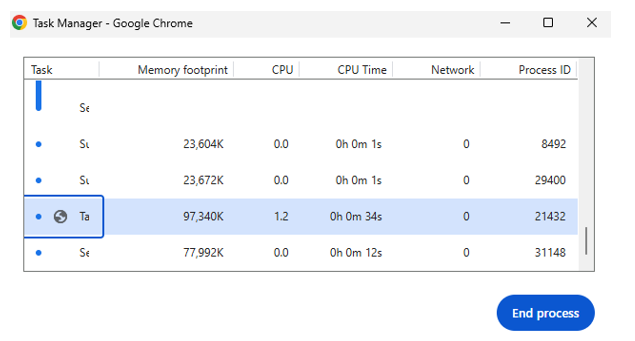
\includegraphics[width=0.8\linewidth]{gambar/Metodologi/Task Manager.png}
		\caption{Pengukuran Footprint Memory}
		\label{Pengukuran Footprint Memory}
	\end{figure}
	
	\item Penggunaan CPU
	 
	Penggunaan CPU diukur dengan library psutil pada Python yang memungkinkan pengukuran pada penggunaan CPU dari task manager. Pengukuran ini merujuk pada penelitian yang dilakukan oleh Vayadande, dkk dalam karyanya yang berjudul “Efficient System for CPU Metric Visualization”[38]. Dalam penelitiannya, pengukuran performa CPU dilakukan secara menyeluruh terhadap seluruh sistem melalui Task Manager. Namun, dalam studi ini, pengukuran akan difokuskan secara lebih spesifik pada penggunaan CPU oleh proses tertentu, dengan merujuk pada PID (Process ID) dari tab atau aplikasi yang dimaksud. Pendekatan ini memungkinkan analisis performa yang lebih terarah dan akurat terhadap aktivitas CPU pada proses yang relevan.
	
	\item Skalabilitas
	
	Skalabilitas akan mengukur perubahan yang terjadi terhadap performa rendering, penggunaan memori, dan penggunaan CPU. Hasilnya, skalabilitas meninjau perubahan tersebut dan memvisualisasikan ke dalam bentuk diagram agar mudah dibandingkan. Pengukuran ini mengacu pada penelitian yang dilakukan oleh Persson dalam judul “Scalability of JavaScript Libraries for Data Visualization” \cite{Persson2021}.
	Untuk meninjau hasil evaluasi performa dan skalabilitas sistem, pengambilan data hasil ukur akan dilakukan pada setiap kelipatan 100. Dalam konteks ini, ukuran data yang diuji dimulai dari 100, 200, 300, 400, 500, dan seterusnya, disesuaikan dengan kapasitas dan batas kemampuan alat uji. Pendekatan bertahap ini bertujuan untuk mengamati sejauh mana sistem mampu mempertahankan performanya seiring dengan meningkatnya beban kerja secara sistematis.	
\end{enumerate}

\subsection{Analisis dan Komparasi}
Tahap analisis dan komparasi merupakan langkah di mana penulis akan mengevaluasi serta membandingkan kinerja dari berbagai library yang telah diimplementasikan dalam penelitian. Pada tahap ini, perbandingan akan dilakukan secara sistematis dengan memanfaatkan visualisasi grafik yang mencakup berbagai parameter sebagai dasar evaluasi. Parameter-parameter tersebut akan digunakan untuk mengukur sejauh mana masing-masing library dapat memenuhi kriteria yang telah ditetapkan, sehingga dapat diperoleh gambaran yang jelas mengenai keunggulan dan kelemahan dari setiap library yang diuji dengan parameter rata-rata waktu render di setiap titik tertentu, rata-rata alokasi memori footprint di titik tertentu, dan rata-rata penggunaan cpu di titik tertentu.

\chapter[HASIL DAN PEMBAHASAN]{\\HASIL DAN PEMBAHASAN}

\section{Perancangan Front End}
Pada tahap perancangan Frontend, penulis menggunakan HTML, CSS, dan Javascript yang diimplementasikan pada framework Laravel. Dari rancangan desain yang telah dibuat, terdapat dua halaman utama dan beberapa function yang mengeksekusi program, seperti fetch API, menampilkan dropdown yang berisi parameter dari API yang di-generate, membuat visualisasi dengan library, dan lainnya. 

\subsection{Halaman Utama}
Pada halaman ini, terdapat beberapa fitur dan fungsi Javascript untuk menjalankan fungsionalitas website. Potongan kode berikut berfungsi untuk men-generate keys yang ada di dalam API yang diinputHakan dari tampilan yang dibuat menggunakan HTML. 
	\begin{figure}[H]
	\centering
	\includegraphics[width=0.8\linewidth]{gambar/Pembahasan/generate API.png}
	\caption{Generate API}
	\label{Generate API}
\end{figure}

Fungsi yang ada pada potongan kode diatas adalah fungsi generateAPI(). Script Javascript yang disusun untuk fungsi tersebut adalah seperti berikut :
	\begin{figure}[H]
	\centering
	\includegraphics[width=0.8\linewidth]{gambar/Pembahasan/fungsi Generate.png}
	\caption{Fungsi Generate API}
	\label{Fungsi Generate API}
\end{figure} 

Kode JavaScript di atas dibuat untuk mengambil data dari API yang dimasukkan oleh pengguna melalui kolom input, lalu menampilkan daftar checkbox berdasarkan kunci-kunci (keys) dari data yang diperoleh. Jika tidak ada input API pada kolom dengan id = “api-input”, sistem akan menampilkan peringatan agar pengguna memasukkan URL yang valid.\\
 
Berikutnya, API akan diambil dengan menggunakan fungsi fetch(). Fetch sendiri merupakan sebuah fungsi bawaan Javascript yang digunakan mengambil data dari sumber eksternal, seperti API, file JSON, atau file lain yang tersedia di server.  Jika respons API gagal, maka sistem akan menampilkan error dan menghentikan proses lebih lanjut. Namun, jika data berhasil diperoleh, sistem akan mengolahnya untuk mendapatkan daftar keys. Setelah daftar keys diperoleh, untuk setiap key, sistem akan menambahkan elemen input bertipe checkbox kemudian tiap checkbox diberi atribut id dan value sesuai dengan key yang bersangkutan sehingga data tersimpan sebagai pasangan key-value. Setelah itu, elemen-elemen ini akan ditempatkan dalam div utama yang memiliki id="api-keys", sehingga checkbox dapat ditampilkan di halaman main page. 
Jika terdapat kesalahan saat mengambil data dari API, error akan dicatat dan ditampilkan di console, dan sistem akan menampilkan peringatan bahwa pengambilan data gagal melalui alert. Dengan fitur ini, pengguna dapat melihat keys pada API secara langsung dan dapat memilih key yang dibutuhkan melalui checkbox yang disediakan. 
	\begin{figure}[H]
	\centering
	\includegraphics[width=0.8\linewidth]{gambar/Pembahasan/use Feature.png}
	\caption{Generate API}
	\label{Fungsi Use Feature}
\end{figure}
Setelah pengguna memilih keys dari checkbox dan menekan tombol “use features” dengan id=“addfeatures”, data akan disimpan di localStorage untuk ditampilkan pada halaman visualisasi. 


\subsection{Halaman Visualisasi}
Pada halaman visualisasi, kode dari fitur dan fungsi digunakan untuk menampilkan dan menambahkan visualisasi secara dinamis dalam sebuah container. 
\begin{enumerate}[label={\alph*.}]
	\item Fungsi Log Render \\
Kode berikut merupakan fungsi untuk mencatat dan menyimpan log waktu rendering setiap grafik yang dihasilkan oleh library visualisasi data. Fungsi ini memastikan bahwa setiap proses pembuatan dan pembaruan grafik terdokumentasi dengan baik, sehingga dapat digunakan untuk analisis performa dan evaluasi efisiensi rendering secara berkala.
		\begin{figure}[H]
	\centering
	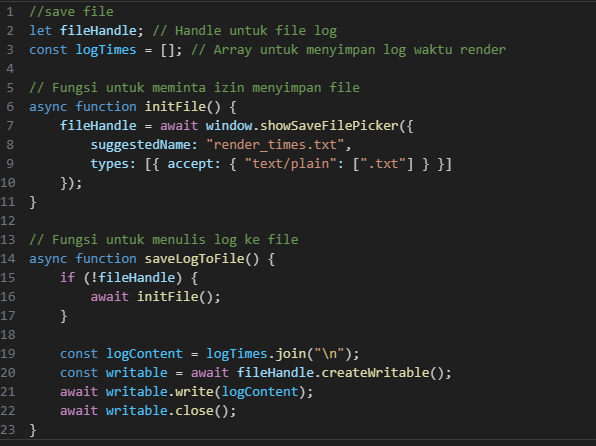
\includegraphics[width=0.8\linewidth]{gambar/Pembahasan/menyimpan log.png}
	\caption{Fungsi Menyimpan Log Render}
	\label{Fungsi Menyimpan Log Render}
	\end{figure} 
	\item Fungsi Fetch Data\\
	Kode JavaScript pada gambar berikut berfungsi untuk mengambil data sensor dari API yang disimpan secara lokal secara berkala dan memperbarui tampilan grafik dengan data terbaru. 
		\begin{figure}[H]
		\centering
		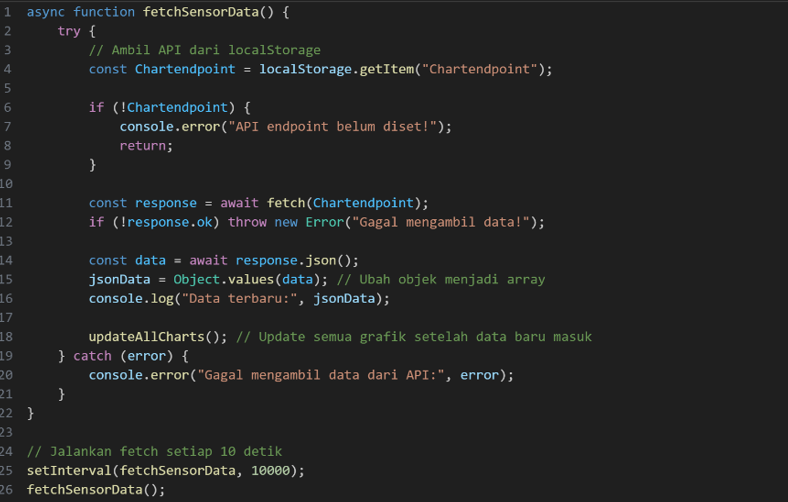
\includegraphics[width=0.8\linewidth]{gambar/Pembahasan/Fungsi Fetch Data.png}
		\caption{Fungsi Fetch Data}
		\label{Fungsi Fetch Data}
	\end{figure} 
	
	Data akan diperbarui dengan menggunakan fungsi bawaan setInterval(fetchSensorData, 10000) yang akan memanggil fetchSensorData() setiap 10 detik. Pada konteks ini, fetchSensorData() bersifat asinkron untuk memastikan proses pengambilan data tidak menghambat eksekusi kode lainnya. Jika respons dari API tidak berhasil, fungsi akan menampilkan eror. 
	Jika data berhasil diambil, tampilan grafik akan diperbarui dengan pemanggilan fungsi updateAllCharts(). Fungsi ini akan memanggil fungsi UpdateChart untuk memperbarui visualisasi pada id chart tertentu.
		\begin{figure}[H]
		\centering
		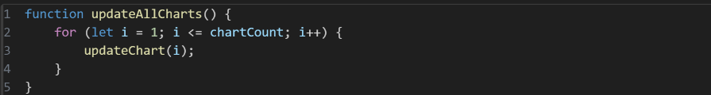
\includegraphics[width=0.8\linewidth]{gambar/Pembahasan/update all data.png}
		\caption{Memperbarui Data pada Chart}
		\label{Memperbarui Data pada Chart}
	\end{figure} 

	
	\item fungsi AddNewVisualization()\\
	Ketika tombol “add new visualization” pada halaman ditekan, fungsi addNewVisualization() akan menambahkan elemen baru ke dalam div dengan id='visualizations' berupa template chart.
		\begin{figure}[H]
		\centering
		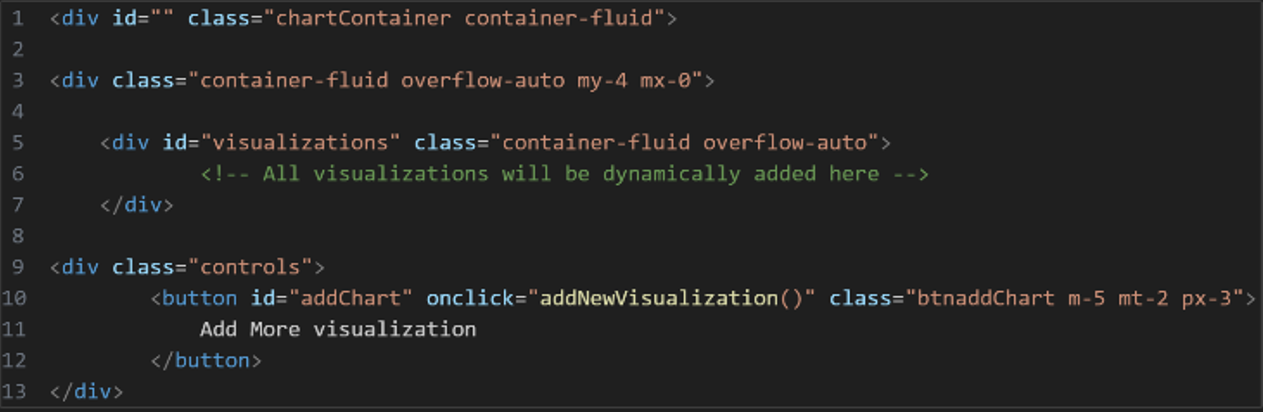
\includegraphics[width=0.8\linewidth]{gambar/Pembahasan/button new visualization.png}
		\caption{Potongan Kode Pada Button New Visualization}
		\label{Potongan Kode Pada Button New Visualization}
	\end{figure}
	
	Tombol dengan id addChart pada event onclick diatas, akan mengeksekusi fungsi addNewVisualization() berikut :
	
	\begin{figure}[H]
		\centering
		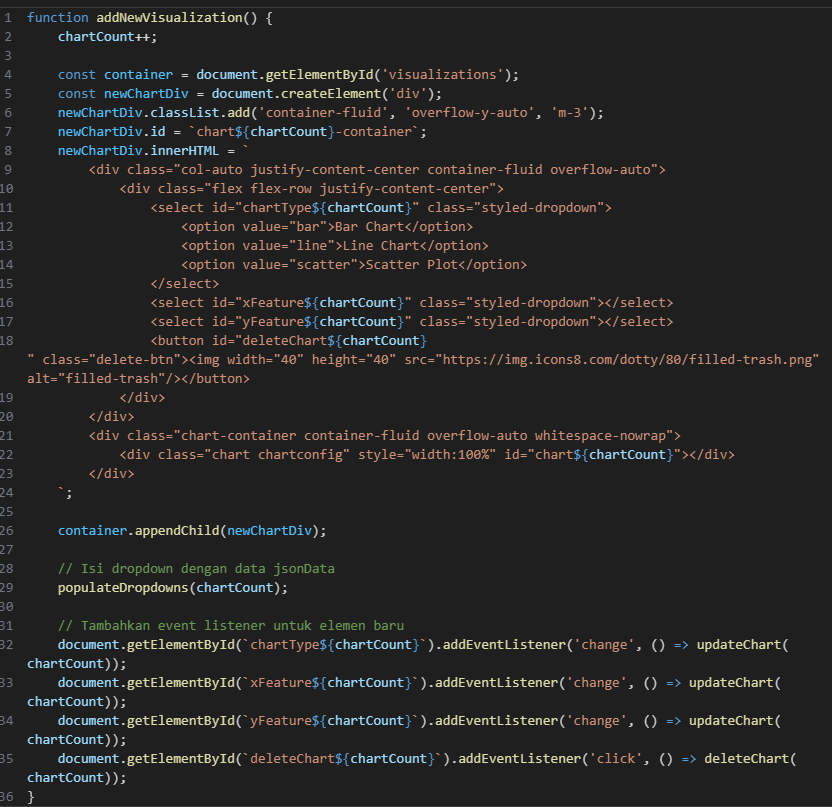
\includegraphics[width=0.8\linewidth]{gambar/Pembahasan/Fungsi new visualization.png}
		\caption{Fungsi untuk Membuat Visualisasi Baru}
		\label{Fungsi untuk Membuat Visualisasi Baru}
	\end{figure}
	Setiap kali fungsi addNewVisualization() dipanggil, variabel chartCount akan menambahkan elemen baru pada wadah div dengan id= “visualizations”. Di dalam elemen <div> yang baru dibuat terdapat dua dropdown yang memungkinkan pengguna memilih tipe grafik (bar, line, atau scatter plot) dan fitur yang akan divisualisasikan. Setiap dropdown memiliki id yang mengandung nilai chartCount agar tidak mengubah visualisasi yang lain ketika terdapat perubahan. Selain itu, terdapat tombol delete yang memungkinkan pengguna menghapus visualisasi tertentu dengan mengklik ikon “trash”.\\
	Setelah struktur HTML untuk visualisasi baru selesai dibuat, elemen tersebut dimasukkan ke dalam container utama menggunakan appendChild(). Fungsi populateDropdowns(chartCount) kemudian dipanggil untuk mengisi dropdown dengan data yang sesuai. 
	
	\item Fungsi PopulateDropdown()\\
	Untuk menampilkan dropdown yang datanya diambil dari data-data API, diperlukan fungsi populateDropdowns(chartCount) seperti pada gambar berikut : 
		\begin{figure}[H]
		\centering
		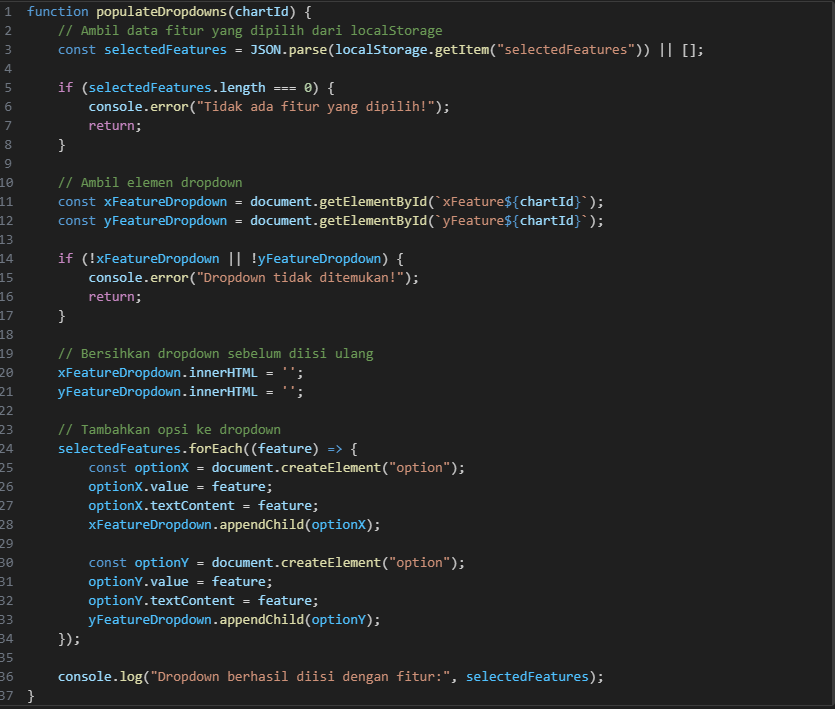
\includegraphics[width=0.8\linewidth]{gambar/Pembahasan/fungsi_populate_dropdown.png}
		\caption{Fungsi untuk Populate Dropdown}
		\label{Fungsi untuk Populate Dropdown}
	\end{figure}
	fungsi ini mengambil data fitur yang telah dipilih sebelumnya dari localStorage.getItem("selectedFeatures"). Jika tidak ada data yang tersimpan, maka variabel selectedFeatures akan berisi array kosong dan sistem akan menunjukkan eror pada console. Kemudian, fungsi ini akan mencocokkan elemen dropdown dengan chartid. Jika salah satu elemen tidak ditemukan, akan muncul pesan eror di console, dan fungsi akan berhenti. Jika elemen dropdown sesuai dengan chartid dan selectedFeatures tidak kosong, selanjutnya fungsi akan menambahkan keys ke dalam dropdown berdasarkan daftar selectedFeatures.
	\item Fungsi CreateChart()\\
	Fungsi createChart() merupakan fungsi yang digunakan untuk menambahkan kode visualisasi sesuai dengan library yang akan diujicobakan.
	\item fungsi UpdateChart()
	 Merupakan fungsi yang digunakan untuk memperbarui grafik secara dinamis berdasarkan data JSON yang ada atau saat fitur pada dropdown diubah. Fungsi ini juga disesuaikan dengan library yang diuji cobakan. 
	fungsi ini mengambil input dari elemen HTML untuk menentukan jenis grafik (chartType), fitur yang akan digunakan sebagai sumbu x (xFeature), dan fitur untuk sumbu y (yFeature) dari array JSON. Data untuk sumbu x disimpan dalam variabel labels, sedangkan data untuk sumbu y disimpan dalam chartData. Keduanya diperoleh menggunakan map(), yang mengambil nilai dari properti yang sesuai dalam objek JSON berdasarkan fitur yang dipilih. Setelah data diperoleh, fungsi createChart(chartId, chartType, labels, chartData) akan dipanggil untuk membuat atau memperbarui grafik dengan data terbaru. 
	\item Fungsi DeleteChart()\\
	Fungsi ini akan memeriksa grafik yang akan dihapus berdasarkan id-nya. Kemudian, grafik akan dihapus dengan fungsi destroy(). Referensi terhadap grafik tersebut juga akan dihapus dari objek chartInstances menggunakan delete chartInstances[chartId]. 
		 \begin{figure}[H]
		\centering
		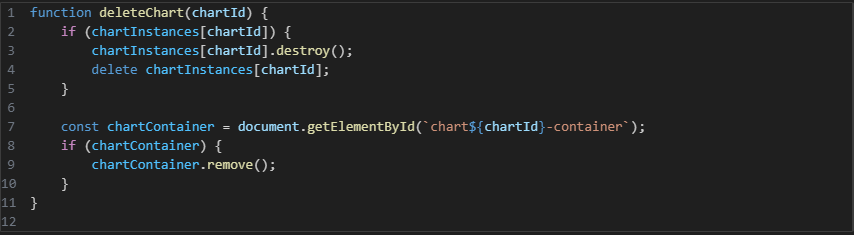
\includegraphics[width=0.8\linewidth]{gambar/Pembahasan/delete-chart.png}
		\caption{Fungsi Delete Chart}
		\label{Fungsi Delete Chart}
		\end{figure}
	\end{enumerate}
	
\section{Implementasi Library}
\subsection{Implementasi Pada Chart.js}
Tahap awal implementasi pada Chart.js dilakukan dengan pembuatan struktur Chart.js pada fungsi createChart(). Fungsi utama dalam kode ini adalah createChart(chartId, chartType, labels, data), yang menerima empat parameter, yaitu chartId untuk memberi id grafik yang akan dibuat, chartType untuk mendefinisikan jenis chart yang akan dibuat, labels untuk menandakan sumbu x, dan variabel data yang akan ditampilkan di dalam grafik sumbu y,  Konfigurasi grafik mencakup tampilan responsif (responsive: true) agar grafik dapat menyesuaikan ukuran layar, skala sumbu x dan y (scales) yang mengatur tampilan label, rotasi teks, serta padding, layout (layout) untuk mengatur jarak padding grafik terhadap batas kanvas, dan Fitur tooltip untuk menampilkan informasi saat pengguna mengarahkan kursor ke grafik.
\begin{enumerate}
	\item Inisialisasi Variabel
	\begin{figure}[H]
		\centering
		\includegraphics[width=0.8\linewidth]{gambar/Pembahasan/Init variabel cjss.png}
		\caption{Inisialisasi Variabel dan Pengukuran Performa}
		\label{Inisialisasi Variabel dan Pengukuran Performa}
	\end{figure}
	
	\item Menentukan Tipe Chart
	\begin{figure}[H]
		\centering
		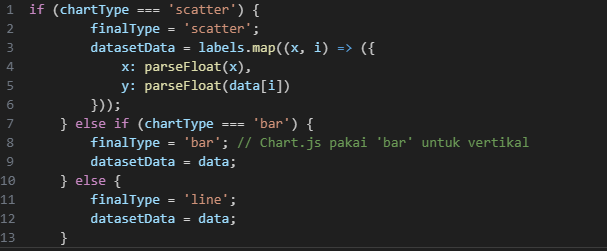
\includegraphics[width=0.8\linewidth]{gambar/Pembahasan/type visual.png}
		\caption{Potongan Kode untuk Menentukan Jenis Visualisasi}
		\label{Potongan Kode untuk Menentukan Jenis Visualisasi}
	\end{figure}
	Potongan kode diatas berfungsi untuk menyesuaikan jenis grafik dan format data yang akan ditampilkan menggunakan Chart.js. Jenis grafik yang akan ditampilkan disesuaikan dengan tipe visualisasi yang dipilih. Pada kondisi ini, data tetap digunakan dalam bentuk array numerik tanpa perlu mengubah strukturnya. Apabila jenis grafik yang dipilih bukan scatter maupun bar, maka secara bawaan tipe grafik diatur menjadi 'line' dengan data yang juga tetap berupa array numerik. 
	
	\item Pembuatan Chart
		\begin{figure}[H]
		\centering
		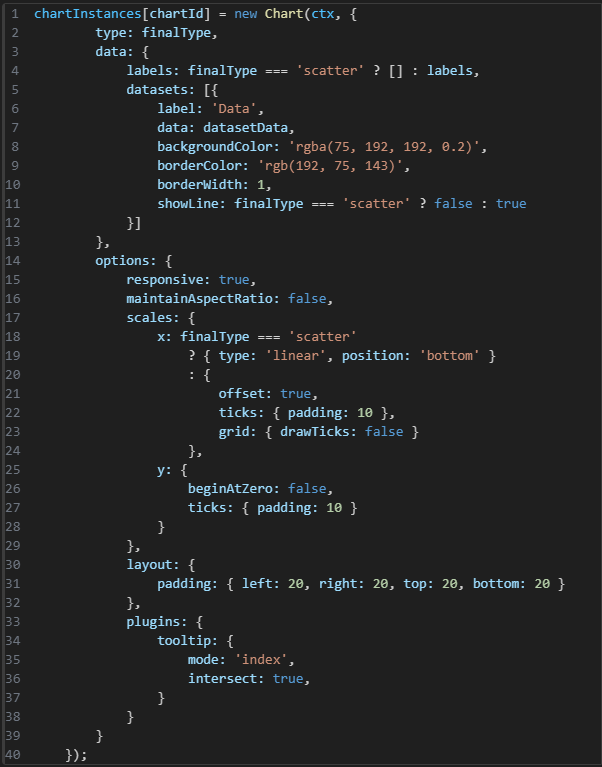
\includegraphics[width=0.8\linewidth]{gambar/Pembahasan/Chartinstance cjs.png}
		\caption{Potongan Kode untuk Pembuatan Chart}
		\label{Potongan Kode untuk Pembuatan Chart}
	\end{figure}
	Potongan kode di atas merupakan bagian dari pembuatan objek grafik baru dengan Chart.js, yang disimpan di dalam `chartInstances` menggunakan `chartId` sebagai \textit{identifier}. Pada bagian `type`, nilai `finalType` digunakan untuk menentukan jenis grafik sesuai hasil logika sebelumnya. Struktur data grafik juga menyesuaikan: jika tipe grafik scatter, maka `labels` dibiarkan kosong karena Chart.js tidak memerlukan sumbu kategori untuk scatter plot, sedangkan pada tipe lain seperti bar dan line, `labels` diisi dengan data kategori sumbu X. Selain itu, pengaturan dataset disesuaikan melalui properti `showLine`, yang akan bernilai `false` khusus untuk scatter agar titik data tidak dihubungkan oleh garis, dan `true` untuk jenis grafik lainnya. Pada bagian `options`, properti `responsive` dan `maintainAspectRatio` memastikan grafik tetap menyesuaikan ukuran layar dengan proporsi yang diatur. Bagian `scales` juga dibuat fleksibel: jika tipe scatter, maka sumbu X diatur sebagai sumbu linear pada posisi bawah. Sedangkan pada tipe lainnya, sumbu X diformat sebagai sumbu kategori dengan pengaturan tampilan tambahan seperti jarak dan grid. Bagian `layout` digunakan untuk memberikan jarak tepi di sekitar area grafik, sedangkan `plugins.tooltip` mengatur perilaku penampilan tooltip agar lebih informatif saat pengguna berinteraksi dengan grafik. Dengan rangkaian pengaturan ini, grafik yang ditampilkan akan memiliki format visual yang benar sesuai tipe data dan kebutuhan pengguna, serta tetap responsif terhadap perubahan tampilan layar.
	
	\item Fungsi Update Chart\\
		\begin{figure}[H]
		\centering
		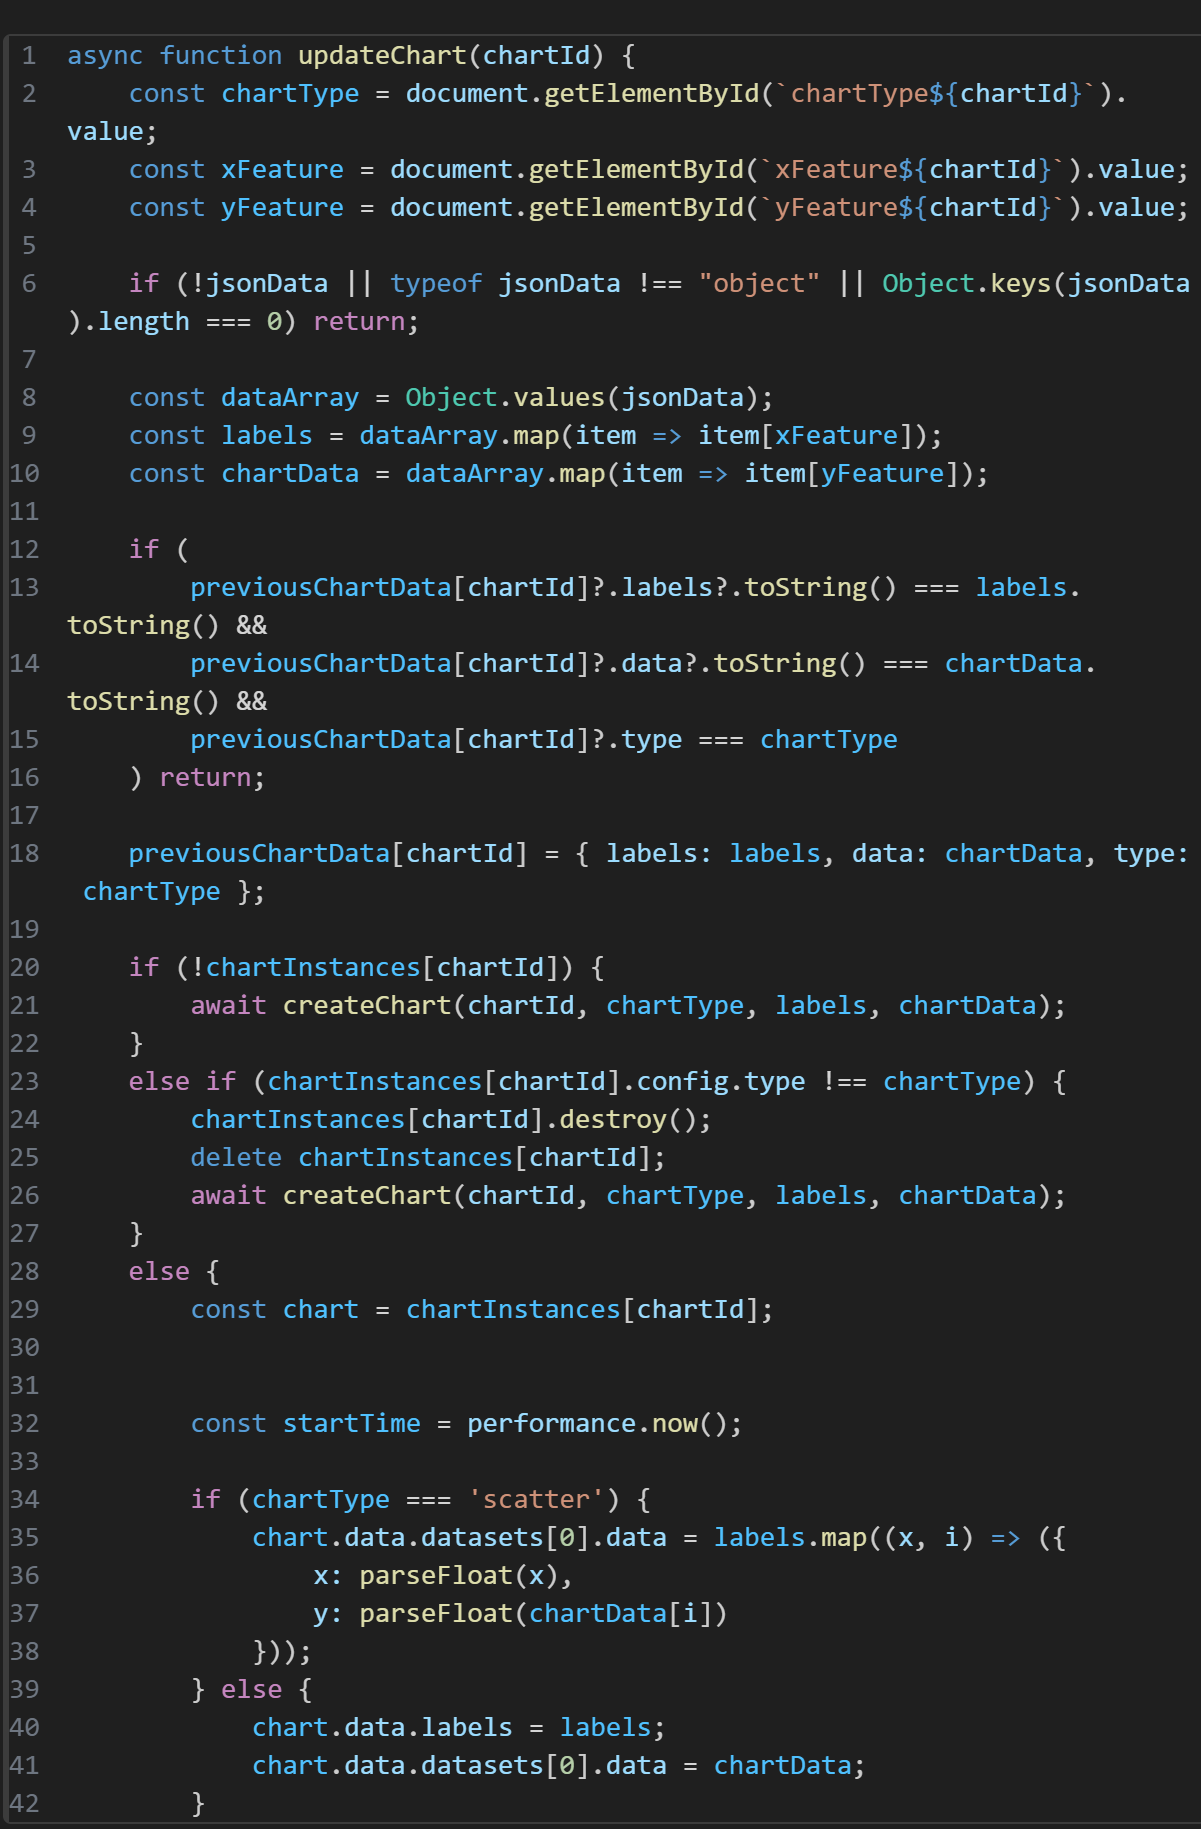
\includegraphics[width=0.8\linewidth]{gambar/Pembahasan/update data cjs.png}
		\caption{Potongan Kode untuk Pembuatan Chart}
		\label{Potongan Kode untuk Pembuatan Chart}
	\end{figure}
	
	Fungsi `updateChart` ini pada dasarnya bertugas memastikan setiap grafik yang tampil selalu mengikuti data sensor terbaru dan pengaturan yang dipilih pengguna. Fungsi akan mengidentifikasi tipe grafik,fitur pada sumbu x, dan fitur pada sumbu y dari dropdown yang berkaitan dengan ID grafik tertentu.\\
	Jika grafik belum ada sama sekali, grafik baru dibuat. Jika tipe grafik diubah, grafik lama dihapus dan diganti dengan grafik baru agar sesuai tipe, dan jika hanya datanya yang berubah, label dan isi datanya diperbarui tanpa perlu membongkar grafik dari awal. 
\end{enumerate}

\subsection{Implementasi Pada D3}
Implementasi pada D3.js dilakukan dengan mengubah fungsi CreateChart() pada kode yang telah dibuat sebelumnya. Penjelasan kode yang diubah adalah sebagai berikut : \\
\begin{enumerate}
	\item Melakukan inisialisasi dan mengatur ukuran chart. Kemudian mengubah sumbu x menjadi scale band yang dapat menerima data kategorikal dan sumbu y menjadi linear agar dapat menampilkan data numerik kontinyu. Kemudian membuat sumbu x dan sumbu y dengan menerapkan beberapa atribut. Seperti pada sumbu x, atribut yang diterapkan adalah translate untuk memindahkan sumbu menjadi dibaagian bawah, memutar teks pada sumbu x dan mengatur font, serta memberikan filter untuk menampilkan keterangan di sumbu x. Adapun atribut yang diterapkan di sumbu y adalah d3.axisLeft tickValues(uniqueYValues) membatasi label sumbu y hanya pada nilai-nilai tertentu.
	\begin{figure}[H]
		\centering
		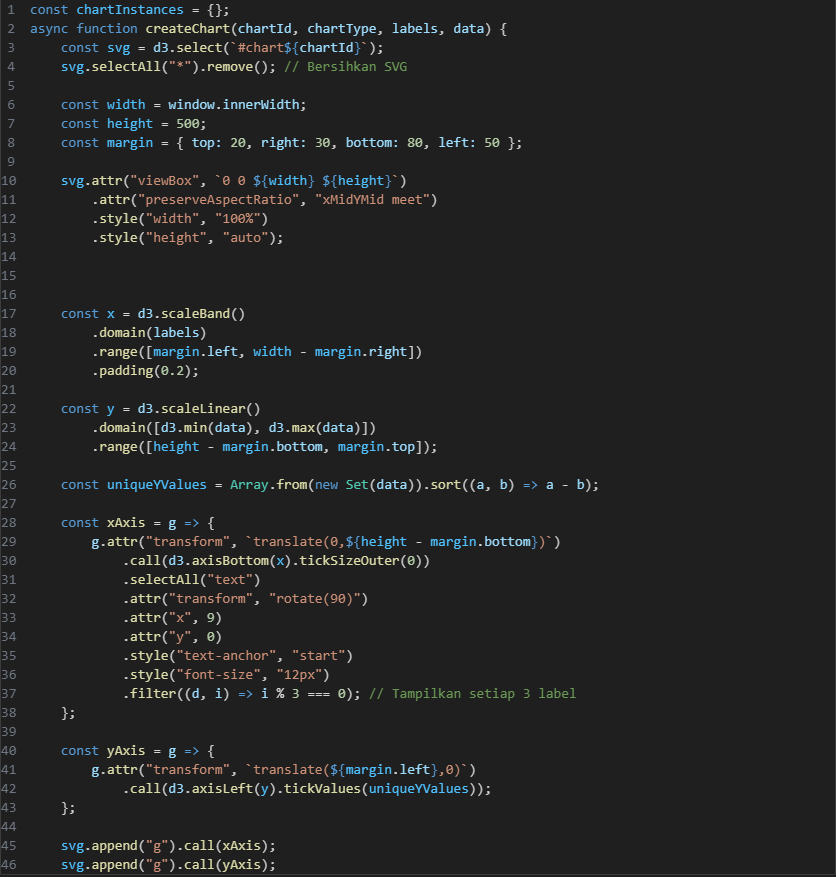
\includegraphics[width=0.8\linewidth]{gambar/Pembahasan/create axis d3.png}
		\caption{Membuat Sumbu Pada D3}
		\label{Membuat Sumbu Pada D3}
	\end{figure}
	\item Menyediakan tooltip yang akan ditampilkan saat kursor di hover ke titik data pada chart.
	\begin{figure}[H]
		\centering
		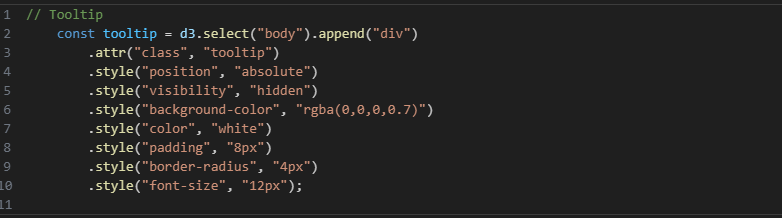
\includegraphics[width=0.8\linewidth]{gambar/Pembahasan/Create Tooltip.png}
		\caption{Potongan Kode untuk Membuat Tooltip }
		\label{Potongan Kode untuk Membuat Tooltip }
	\end{figure} 
	\item Menambahkan visualisasi berdasarkan jenis grafik yang akan dipilih (line chart, bar chart, atau scatter plot). Kode berikut membuat grafik garis (line chart). Pertama, dibuat jalur garis menggunakan d3.line() berdasarkan data dan label yang dipetakan ke sumbu x dan y. Kemudian, titik-titik data ditampilkan sebagai titik merah. Setiap titik memiliki interaksi tooltip yang muncul saat pointer diarahkan ke titik dan akan menampilkan informasi sumbu x dan sumbu y.
	\begin{figure}[H]
		\centering
		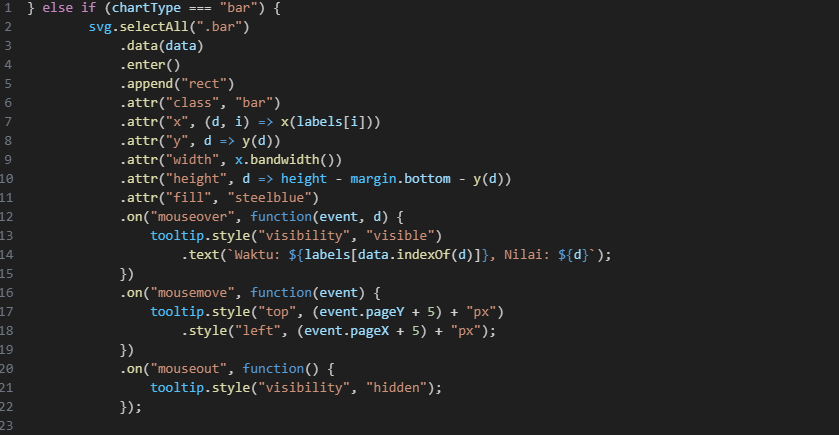
\includegraphics[width=0.8\linewidth]{gambar/Pembahasan/implementasi bar chart.png}
		\caption{Potongan Kode untuk Mengimplementasikan Line Chart}
		\label{Potongan Kode untuk Mengimplementasikan Line Chart}
	\end{figure}
	\item Membuat grafik diagram batang dengan elemen rect. Pada kode berikut posisi batang diatur dengan .attr("x", ...) berdasarkan label dan skala data x. Tinggi batang dihitung dari selisih tinggi SVG dan posisi data pada sumbu y, sementara lebar batang diambil dari x.bandwidth(). 
	\begin{figure}[H]
		\centering
		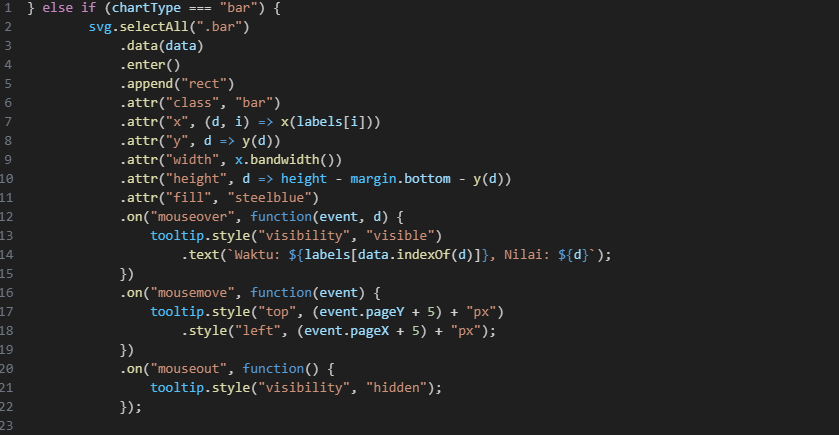
\includegraphics[width=0.8\linewidth]{gambar/Pembahasan/implementasi bar chart.png}
		\caption{Potongan Kode untuk Mengimplementasikan Bar Chart}
		\label{Potongan Kode untuk Mengimplementasikan Bar Chart}
	\end{figure}
	\item Membuat grafik scatter plot, dengan menentukan posisi x dan y. Masing-masing titik digambar sebagai lingkaran berwarna kuning dengan garis tepi hitam. Tooltip interaktif juga digunakan, sama seperti pada grafik batang, untuk menunjukkan informasi detail saat pointer diarahkan ke titik.
	\begin{figure}[H]
		\centering
		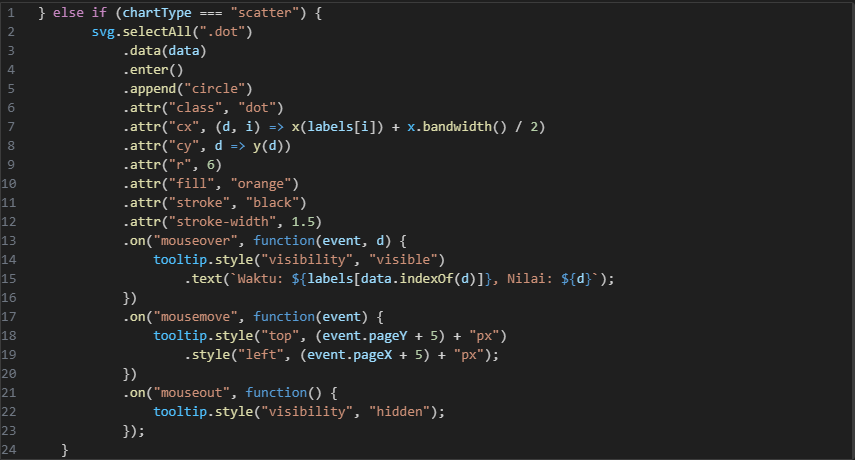
\includegraphics[width=0.8\linewidth]{gambar/Pembahasan/implementasi scatter plot.png}
		\caption{Potongan Kode untuk Mengimplementasikan Scatter Plot}
		\label{Potongan Kode untuk Mengimplementasikan Scatter Plot}
	\end{figure}
	
	\item Fungsi Update Pada D3
		\begin{figure}[H]
		\centering
		\includegraphics[width=0.8\linewidth]{gambar/Pembahasan/Fungsi Update D3.png}
		\caption{Fungsi untuk Memperbarui Chart D3}
		\label{Fungsi untuk Memperbarui Chart D3}
	\end{figure}
	Fungsi diatas akan mengambil informasi dari elemen HTML berupa tipe grafik, nama fitur untuk sumbu X, dan fitur untuk sumbu Y berdasarkan ID grafik yang sedang diproses. Setelah itu, fungsi memeriksa apakah jsonData yang berisi data sensor sudah valid, berupa objek, dan memiliki isi. Jika data tidak ada atau tidak sesuai format, fungsi akan menghentikan proses dan mencatat pesan kesalahan ke konsol untuk memudahkan pengecekan. Kemudian objek JSON diubah menjadi array agar lebih mudah diolah. Jika array ini kosong, berarti tidak ada data valid yang dapat divisualisasikan, sehingga fungsi kembali membatalkan proses dan menampilkan error. Kemudian, data untuk sumbu X dan Y diambil masing-masing dengan melakukan mapping ke array fitur X menjadi label, dan fitur Y menjadi data nilai.	
\end{enumerate}



\subsection{Implementasi Pada Highcharts}
Implementasi Highcharts dilakukan pada fungsi CreateChart() dengan menambahkan kode berikut.\\
\begin{enumerate}
\item Implementasi Kontainer Grafik\\
 Pertama, kode membuat id kontainer grafik. Jika grafik dengan chartId yang sama sudah pernah dibuat sebelumnya, maka grafik lama akan dihapus menggunakan fungsi destroy() untuk mencegah duplikasi. 
		\begin{figure}[H]
	\centering
	\includegraphics[width=0.8\linewidth]{gambar/Pembahasan/Init Highcharts.png}
	\caption{Potongan Kode untuk Kontainer Grafik}
	\label{Potongan Kode untuk Kontainer Grafik}
\end{figure}
\item Implementasi ChartOptions\\
Selanjutnya, objek chartOptions disusun sebagai konfigurasi grafik. Pada bagian chart, properti renderTo menunjukkan elemen HTML yang menjadi wadah grafik, sementara type diisi dengan tipe grafik dari variabel highchartsType yang sudah ditetapkan. 
		\begin{figure}[H]
	\centering
	\includegraphics[width=0.8\linewidth]{gambar/Pembahasan/Membuat chart highcharts.png}
	\caption{Potongan Kode untuk Membuat Grafik Highcharts}
	\label{Potongan Kode untuk Membuat Grafik Highcharts}
\end{figure}

Properti zoomType diaktifkan agar pengguna dapat melakukan pembesaran tampilan grafik pada sumbu horizontal dan vertikal. Untuk sumbu X (xAxis), apabila grafik berjenis scatter, properti categories diatur null karena scatter plot memanfaatkan nilai numerik langsung, bukan kategori. Sebaliknya, untuk jenis grafik lain, labels digunakan sebagai penanda kategori. Judul pada sumbu X dan Y diatur berdasarkan input fitur X dan Y yang dipilih pengguna melalui elemen HTML.

Bagian series berfungsi menentukan data yang akan divisualisasikan. Jika grafik bertipe scatter, data diolah menjadi pasangan nilai [x, y] dengan format numerik melalui parseFloat. Untuk tipe grafik lain, data digunakan sebagaimana adanya. Di bagian responsive, terdapat aturan tambahan yang akan menyembunyikan legenda grafik secara otomatis jika lebar layar di bawah 600 piksel, sehingga tampilan tetap rapi pada perangkat berlayar kecil. Kemudian, perintah Highcharts.chart(chartOptions) akan merender grafik sesuai pengaturan tersebut ke dalam halaman. Hasil grafik ini kemudian disimpan ke dalam chartInstances[chartId] agar dapat diakses dan diperbarui. 

\item Update Highcharts\\
 Fungsi updateChart yang berfungsi untuk memperbarui data grafik berdasarkan fitur yang dipilih. Langkah kerjanya dimulai dengan mengambil jenis grafik serta nama fitur untuk sumbu X dan Y dari elemen HTML. Kemudian, fungsi akan memvalidasi jsonData. Selanjutnya, data JSON dikonversi menjadi array, lalu dipecah menjadi data sumbu X (labels) dan data sumbu Y (chartData). Jika hasil ekstraksi data kosong atau gagal, fungsi juga akan berhenti sambil menampilkan pesan error. Terakhir, jika semua valid, data tersebut akan dipakai untuk membuat atau memperbarui grafik.
 		\begin{figure}[H]
 	\centering
 	\includegraphics[width=0.8\linewidth]{gambar/Pembahasan/Update Highcharts.png}
 	\caption{Potongan Kode untuk Memperbarui Grafik Highcharts}
 	\label{Potongan Kode untuk Memperbarui Grafik Highcharts}
 \end{figure}
\end{enumerate}


\section{Pengukuran Performa Rendering}
Pada bagian ini, dilakukan pengukuran performa rendering untuk menilai seberapa efisien dan responsif library dalam menampilkan data visualisasi. Pengujian dilakukan dengan menggunakan beberapa skenario jumlah data yang ditampilkan melalui line chart untuk mengamati waktu yang dibutuhkan dalam merender grafik ke layar. Proses pengukuran dilakukan dengan mencatat waktu rendering sejak inisialisasi data hingga grafik ditampilkan secara penuh di DOM. Analisis ini bertujuan untuk memberikan gambaran kuantitatif mengenai kemampuan library dalam menangani berbagai skenario penggunaan, serta menjadi dasar perbandingan dengan library visualisasi data lainnya. Pengujian dilakukan sebanyak tiga kali eksperimen untuk menentukan library paling optimal dan guna menghilangkan bias dalam pengukuran kemudian hasil pengujian tersebut dibandingkan dalam tabel yang berisi jumlah sampel, hasil eksperimen pertama (1st), hasil eksperimen kedua (2nd) dan hasil eksperimen ketiga (3rd). 

\subsection{Chart.js}
Pengukuran ini dilakukan untuk mengevaluasi performa Chart.js dalam merender berbagai jenis grafik dengan jumlah data yang bervariasi. Waktu rendering dihitung mulai dari proses inisialisasi chart hingga seluruh elemen visual berhasil ditampilkan pada halaman. Hasil rendering dengan library Chart.js sebanyak tiga kali eksperimen adalah sebagai berikut :

\begin{table}[h!]
	\centering
	\caption{Komparasi Render \textit{Chart.js}}
	\label{tab:komparasi_chartjs}
	\renewcommand{\arraystretch}{1.2}
	\begin{tabular}{|c|c|c|c|}
		\hline
		\textbf{Samples} & \textbf{1\textsuperscript{st}} & \textbf{2\textsuperscript{nd}} & \textbf{3\textsuperscript{rd}} \\
		\hline
		100 & 5.36 & 5.46 & 3.00 \\
		200 & 5.19 & 5.35 & 3.27 \\
		300 & 5.56 & 5.54 & 3.58 \\
		400 & 6.10 & 5.77 & 3.86 \\
		500 & 6.40 & 6.20 & 4.13 \\
		600 & 6.42 & 6.50 & 4.41 \\
		700 & 6.66 & 6.92 & 4.72 \\
		\ldots & \ldots & \ldots & \ldots \\
		4400 & 18.33 & 19.23 & 15.25 \\
		4500 & 18.55 & 19.51 & 15.55 \\
		4600 & 18.78 & 19.81 & 15.86 \\
		4700 & 19.72 & 20.10 & 16.40 \\
		4800 & 20.02 & 20.44 & 16.87 \\
		4900 & 20.23 & 20.66 & 17.12 \\
		5000 & 20.43 & 20.91 & 17.37 \\
		\hline
	\end{tabular}
\end{table}

 	\begin{figure}[H]
	\centering
	\includegraphics[width=0.8\linewidth]{gambar/Pembahasan/FIX_Render/render chart js_fix.png}
	\caption{Perbandingan Rendering Chart.js}
	\label{Perbandingan Rendering Chart.js}
\end{figure}

Hasil pengujian waktu render Chart.js pada tiga kali percobaan (1st, 2nd, dan 3rd) menunjukkan pola pertumbuhan yang konsisten seiring bertambahnya jumlah sampel data, dari 100 hingga 5000. Pada sampel terkecil, yaitu 100 data, waktu render pada percobaan pertama tercatat sebesar 5.36 ms, percobaan kedua 5.46 ms, dan percobaan ketiga 3.00 ms. Seiring bertambahnya jumlah data, tren kenaikan pada ketiga percobaan tampak serupa: misalnya pada 1000 data, waktu render untuk percobaan pertama naik menjadi 7.49 ms, percobaan kedua 9.19 ms, dan percobaan ketiga 5.65 ms. Pola yang sama terus berlanjut hingga data terbesar, yaitu 5000 sampel, di mana percobaan pertama mencapai 20.43 ms, percobaan kedua 20.91 ms, sedangkan percobaan ketiga tetap lebih rendah di angka 17.37 ms.

Data ini menunjukkan bahwa meskipun kondisi environment dan skrip yang digunakan sama, selalu muncul deviasi antar percobaan, terutama antara percobaan pertama dan kedua yang cenderung memiliki selisih mendekati stabil di rentang 0.5–1 ms, sedangkan percobaan ketiga relatif lebih cepat dengan selisih 2–3 ms lebih rendah dibanding dua percobaan lainnya. Fenomena ini mengindikasikan bahwa Chart.js mempertahankan konsistensi skalabilitas render di setiap percobaan meskipun ada variasi minor antar iterasi. Kenaikan waktu render mendekati linier sesuai penambahan beban data, yang wajar terjadi karena semakin banyak elemen visual dan kalkulasi yang harus diolah pada browser. Perbedaan antar percobaan kemungkinan besar berkaitan dengan variasi eksekusi di tingkat proses atau pengelolaan memori internal browser, meskipun secara teknis tidak ada perubahan pada sumber kode dan tidak dilakukan optimasi tambahan.

\subsection{D3}
Pengujian ini bertujuan untuk menilai kinerja D3 dalam menampilkan kemampuan rendering library D3 dengan volume data yang berbeda-beda. Proses pengukuran dimulai dari saat chart diinisialisasi hingga seluruh komponen visual sepenuhnya muncul di layar. Untuk memperoleh hasil yang konsisten, proses rendering dilakukan sebanyak tiga kali dengan D3.js. Berikut merupakan grafik perbandingan hasil dari ketiga percobaan tersebut:

\begin{table}[H]
	\centering
	\caption{Komparasi Render D3}
	\label{Komparasi Render D3}
	\renewcommand{\arraystretch}{1.2}
	\begin{tabular}{|c|c|c|c|}
		\hline
		\textbf{Samples} & \textbf{1\textsuperscript{st}} & \textbf{2\textsuperscript{nd}} & \textbf{3\textsuperscript{rd}} \\
		\hline
		100  & 0.35 & 0.58 & 0.40 \\
		200  & 0.62 & 1.05 & 0.79 \\
		300  & 0.59 & 1.50 & 1.13 \\
		400  & 0.60 & 2.03 & 1.66 \\
		500  & 0.73 & 1.81 & 2.03 \\
		600  & 0.93 & 1.72 & 2.39 \\
		700  & 1.26 & 1.80 & 2.77 \\
		\ldots & \ldots & \ldots & \ldots \\
		4400 & 14.91 & 15.69 & 17.38 \\
		4500 & 15.08 & 15.84 & 17.56 \\
		4600 & 15.25 & 15.99 & 17.72 \\
		4700 & 15.44 & 16.14 & 17.89 \\
		4800 & 15.81 & 16.31 & 18.06 \\
		4900 & 16.03 & 16.48 & 18.23 \\
		5000 & 16.23 & 16.66 & 18.41 \\
		\hline
	\end{tabular}
\end{table}

 	\begin{figure}[H]
	\centering
	\includegraphics[width=0.8\linewidth]{gambar/Pembahasan/FIX_Render/d3.png}
	\caption{Perbandingan Rendering D3}
	\label{Perbandingan Rendering D3}
\end{figure}

Berdasarkan hasil pengamatan terhadap data rendering D3.js, ketiga percobaan memperlihatkan pola kenaikan waktu rendering yang konsisten seiring bertambahnya jumlah sampel data. Hal ini wajar mengingat D3.js memanfaatkan manipulasi DOM dan SVG secara intensif, sehingga makin banyak data yang dirender, makin besar pula beban prosesnya. 
Nilai pada percobaan pertama memperlihatkan pola pertumbuhan yang konsisten dan stabil, naik secara bertahap dari 0,35 ms hingga mencapai 16,20 di akhir rentang data, tanpa penurunan. Nilai percobaan kedua juga mengalami peningkatan yang stabil, bahkan lebih cepat dibandingkan pertama dalam beberapa titik data. Dimulai dari 0,58 ms, nilainya terus meningkat hingga menjadi yang tertinggi di titik akhir, yaitu 16,66ms. 
Nilai 3rd menunjukkan tren yang sedikit berbeda. Nilai ini tumbuh paling pesat dan mendominasi mencapai puncaknya di angka 18,41ms.
Meskipun masing-masing memiliki laju pertumbuhan yang berbeda dan pola yang sedikit bervariasi, terutama pada nilai percobaan ketiga yang sempat menurun di akhir, secara umum tren ketiganya tetap mengarah naik.


\subsection{highcharts}
Untuk menilai kemampuan render Highcharts dalam menampilkan berbagai jenis grafik dengan variasi jumlah data, dilakukan proses pengujian dengan mengukur waktu yang dibutuhkan sejak inisialisasi grafik hingga seluruh komponen visual sepenuhnya muncul di layar. Evaluasi ini dilakukan sebanyak tiga kali untuk menampilkan data dengan line chart, dan berikut merupakan hasil yang diperoleh dari penggunaan Highcharts dalam tiga eksperimen tersebut.

\begin{longtable}{|c|c|c|c|}
	\caption{\textit{Komparasi} Render Highcharts} \\
	\hline
	\textbf{Samples} & \textbf{1\textsuperscript{st}} & \textbf{2\textsuperscript{nd}} & \textbf{3\textsuperscript{rd}} \\
	\hline
	\endfirsthead
	\hline
	\textbf{Samples} & \textbf{1\textsuperscript{st}} & \textbf{2\textsuperscript{nd}} & \textbf{3\textsuperscript{rd}} \\
	\hline
	\endhead
100  & 34.35 & 38.80 & 24.57 \\
200  & 37.81 & 40.50 & 28.81 \\
300  & 38.37 & 41.77 & 29.50 \\
400  & 38.67 & 41.93 & 30.17 \\
500  & 38.55 & 41.27 & 30.40 \\
600  & 38.79 & 41.32 & 30.86 \\
700  & 38.53 & 41.20 & 31.26 \\
\ldots & \ldots & \ldots & \ldots \\
4400 & 40.91 & 41.68 & 37.20 \\
4500 & 41.06 & 41.77 & 37.44 \\
4600 & 41.22 & 41.89 & 37.73 \\
4700 & 41.40 & 41.99 & 37.98 \\
4800 & 41.52 & 42.10 & 38.44 \\
4900 & 41.64 & 42.21 & 39.17 \\
5000 & 41.82 & 42.35 & 39.95 \\
	\hline
\end{longtable}
 	\begin{figure}[H]
	\centering
	\includegraphics[width=0.8\linewidth]{gambar/Pembahasan/FIX_Render/hc.png}
	\caption{Perbandingan Rendering Highcharts}
	\label{Perbandingan Rendering Highcharts}
\end{figure}
Ditinjau dari ketiga eksperimen yang dilakukan, waktu render dengan library Highcharts meningkat di awal dan cenderung stabil di data dalam jumlah lebih dari 1000. Hal ini dikarenakan sebuah mekanisme TurboThreshold yang menjadi fitur default di dalam Highcharts yang belum berjalan. Fitur TurboThreshold ini adalah sebuah konfigurasi yang memungkinkan Highcharts untuk memvalidasi setiap titik yang dirender. Defaultnya, fitur ini akan mulai dijalankan secara otomatis saat jumlah data lebih dari 1000. Hal ini menjadi alasan yang valid karena setelah data ke 1000, tidak ada kenaikan waktu render yang signifikan dan kenaikan cenderung landai. 

\section{Pengukuran Penggunaan CPU}
Pengukuran penggunaan CPU ditinjau melalui Process ID (PID) terspesifik pada website. Fungsi dari pengukuraan CPU ini adalah untuk mengukur rata-rata penggunaan CPU saat digunakan untuk merender jumlah data tertentu. Tahapan yang dilakukan dalam pengukuran ini antara lain: 
\begin{enumerate}
	\item Membuka Task Manager pada Chrome untuk melihat PID dari tab yang digunakan. 
	\item Menuliskan PID pada kode yang telah dibuat. Kode ini berfungsi untuk mengambil nilai CPU yang digunakan pada suatu tab setiap detik. 
	 	\begin{figure}[H]
		\centering
		\includegraphics[width=0.8\linewidth]{gambar/Pembahasan/Mengukur CPU.png}
		\caption{Potongan Kode untuk Mengukur Penggunaan CPU}
		\label{Potongan Kode untuk Mengukur Penggunaan CPU}
	\end{figure}
	\item Nilai CPU tersebut kemudian akan disimpan dalam file csv.
\end{enumerate}


\subsection{Chart.js}
Pengukuran penggunaan CPU pada library Chart.js untuk menampilkan data IoT dalam bentuk line chart menunjukkan hasil seperti berikut : 
\begin{longtable}{|c|c|c|c|}
	\caption{Komparasi CPU \textit{Chart.js}} \\
	\hline
	\textbf{Samples} & \textbf{1\textsuperscript{st}} & \textbf{2\textsuperscript{nd}} & \textbf{3\textsuperscript{rd}} \\
	\hline
	\endfirsthead
	\hline
	\textbf{Samples} & \textbf{1\textsuperscript{st}} & \textbf{2\textsuperscript{nd}} & \textbf{3\textsuperscript{rd}} \\
	\hline
	\endhead
	100  & 0.22 & 0.18 & 0.15 \\
	200  & 0.21 & 0.19 & 0.13 \\
	300  & 0.25 & 0.19 & 0.13 \\
	400  & 0.23 & 0.20 & 0.14 \\
	500  & 0.24 & 0.21 & 0.14 \\
	600  & 0.24 & 0.22 & 0.15 \\
	700  & 0.25 & 0.23 & 0.16 \\
	\ldots & \ldots & \ldots & \ldots \\
	4400 & 0.85 & 0.68 & 0.53 \\
	4500 & 0.86 & 0.69 & 0.55 \\
	4600 & 0.87 & 0.70 & 0.56 \\
	4700 & 0.86 & 0.71 & 0.56 \\
	4800 & 0.85 & 0.72 & 0.55 \\
	4900 & 0.86 & 0.73 & 0.54 \\
	5000 & 0.86 & 0.74 & 0.54 \\
	\hline
\end{longtable}

	\begin{figure}[H]
	\centering
	\includegraphics[width=0.8\linewidth]{gambar/Pembahasan/FIX_CPU/cjs compare.png}
	\caption{Grafik Komparasi Chart.js}
	\label{Grafik Komparasi Chart.js}
\end{figure}

Dari ketiga eksperimen yang dilakukan, penggunaan CPU pada library Chart.js untuk menampilkan data IoT memiliki kemiripan. Grafik kenaikan di semua iterasi pun terlihat landai. Hal ini dikarenakan Chart.js menggunakan canvas rendering yang lebih menggunakan resource GPU disbanding CPU.
Dari grafik tersebut, eksperimen kedua menunjukkan peningkatan penggunaan CPU setelah 2900 data. Hal ini dapat mengindikasikan terjadi lonjakan di waktu render dan/atau penggunaan memori. Meskipun begitu, ketiganya konsisten menunjukkan kenaikan penggunaan CPU seiring bertambahnya jumlah data.

\subsection{D3}
Pengukuran penggunaan CPU pada library D3 untuk menampilkan data IoT dalam bentuk line chart menunjukkan hasil seperti berikut : 
\begin{longtable}{|c|c|c|c|}
	\caption{Komparasi CPU \textit{Chart.js}} \\
	\hline
	\textbf{Samples} & \textbf{1\textsuperscript{st}} & \textbf{2\textsuperscript{nd}} & \textbf{3\textsuperscript{rd}} \\
	\hline
	\endfirsthead
	\hline
100  & 0.20 & 0.46 & 0.22 \\
200  & 0.16 & 0.53 & 0.28 \\
300  & 0.14 & 0.64 & 0.35 \\
400  & 0.13 & 0.77 & 0.46 \\
500  & 0.14 & 0.91 & 0.61 \\
600  & 0.16 & 1.03 & 0.74 \\
700  & 0.19 & 1.14 & 0.86 \\
\ldots & \ldots & \ldots & \ldots \\
4400 & 5.10 & 5.56 & 5.64 \\
4500 & 5.21 & 5.46 & 5.75 \\
4600 & 5.33 & 5.36 & 5.74 \\
4700 & 5.45 & 5.44 & 5.73 \\
4800 & 5.57 & 5.57 & 5.73 \\
4900 & 5.70 & 5.71 & 5.74 \\
5000 & 5.83 & 5.84 & 5.76 \\
	\hline
\end{longtable}

	\begin{figure}[H]
	\centering
	\includegraphics[width=0.8\linewidth]{gambar/Pembahasan/FIX_CPU/d3_compare.png}
	\caption{Grafik Komparasi D3}
	\label{Grafik Komparasi D3}
\end{figure}
Ketiga grafik memiliki pola kenaikan yang sama karena peningkatan ukuran data, peningkatan render elemen DOM, dan rendering grafik yang semakin kompleks. Kenaikan CPU pada proses ini mencapai titik tertinggi di 5,8 ms dan tren ini terjadi pada ketiga eksperimen yang dilakukan. 

\subsection{Highcharts}
Pengukuran penggunaan CPU pada library Highcharts untuk menampilkan data IoT dalam bentuk line chart menunjukkan hasil seperti berikut : 
\begin{table}[H]
	\centering
	\caption{Komparasi CPU pada \textit{Highcharts}}
	\begin{tabular}{|c|c|c|c|}
		\hline
		\textbf{Samples} & \textbf{1\textsuperscript{st}} & \textbf{2\textsuperscript{nd}} & \textbf{3\textsuperscript{rd}} \\
		\hline
		100  & 2.28 & 4.30 & 2.83 \\
		200  & 3.84 & 4.22 & 2.79 \\
		300  & 3.92 & 4.13 & 2.86 \\
		400  & 4.31 & 4.43 & 2.89 \\
		500  & 4.78 & 4.76 & 2.97 \\
		600  & 5.09 & 5.10 & 3.04 \\
		700  & 5.40 & 5.39 & 3.13 \\
		\ldots & \ldots & \ldots & \ldots \\
		4400 & 6.00 & 6.77 & 5.13 \\
		4500 & 5.88 & 6.78 & 5.16 \\
		4600 & 5.76 & 6.80 & 5.19 \\
		4700 & 5.65 & 6.81 & 5.14 \\
		4800 & 5.54 & 6.82 & 5.04 \\
		4900 & 5.44 & 6.83 & 4.94 \\
		5000 & 5.34 & 6.84 & 4.85 \\
		\hline
	\end{tabular}
\end{table}

	\begin{figure}[H]
	\centering
	\includegraphics[width=0.8\linewidth]{gambar/Pembahasan/FIX_CPU/hc_compare.png}
	\caption{Grafik Komparasi Highcharts}
	\label{Grafik Komparasi Highcharts}
\end{figure}

Dari ketiga eksperimen yang dilakukan, secara konsisten terdapat peningkatan penggunaan CPU saat data kurang dari 1500 kemudian setelahnya data menjadi lebih stabil atau mengalami penurunan. Hal ini dapat disebabkan oleh fungsi TurboThreshold yang juga turut mempengaruhi performa render dan penggunaan memori. 


\section{Pengukuran Footprint Memory}
Pengukuran penggunaan memori dintinjau dari penggunaan footprint memory pada sebuah halaman website spesifik yang mengukur private memory, heap memory untuk menyimpan objek di dalam website termasuk data dari json yang ditampilkan, dan stack memory untuk menyimpan variabel lokal dan kontrol eksekusi fungsi. Langkah yang dilakukan pada tahap ini adalah sebagai berikut :

\begin{enumerate}
\item Menampilkan visualisasi pada tab incognito 
\item Meninjau penggunaan memory footprint yang dapat diakses melalui Task Manager pada Chrome
\item Mencatat performa di tiap titik yang telah ditentukan, yaitu 100, 200, 300, 400, dan seterusnya hingga data ke 5000
Langkah tersebut dilakukan sebanyak tiga kali eksperimen di tiap-tiap library untuk mengukur penggunaan memorinya.  
\end{enumerate} 
\subsection{Chart.js}
Pengukuran memori pada Chart.js dalam tiga eksperimen menghasilkan grafik perbandingan seperti berikut :
\begin{table}[H]
	\centering
	\caption{Komparasi Memori \textit{Chart.js}}
	\begin{tabular}{|c|c|c|c|}
		\hline
		\textbf{Samples} & \textbf{1\textsuperscript{st}} & \textbf{2\textsuperscript{nd}} & \textbf{3\textsuperscript{rd}} \\
		\hline
		100  & 56{,}730 & 59{,}600  & 56{,}883 \\
		200  & 57{,}460 & 66{,}959  & 58{,}921 \\
		300  & 66{,}104 & 74{,}317  & 60{,}734 \\
		400  & 70{,}215 & 81{,}676  & 62{,}489 \\
		500  & 74{,}326 & 89{,}035  & 64{,}120 \\
		600  & 78{,}437 & 96{,}394  & 65{,}871 \\
		700  & 82{,}548 & 103{,}752 & 67{,}534 \\
		\ldots & \ldots & \ldots & \ldots \\
		4400 & 152{,}967 & 142{,}615 & 146{,}051 \\
		4500 & 155{,}905 & 143{,}490 & 146{,}128 \\
		4600 & 157{,}111 & 144{,}365 & 146{,}152 \\
		4700 & 154{,}744 & 145{,}240 & 146{,}062 \\
		4800 & 156{,}783 & 148{,}564 & 146{,}067 \\
		4900 & 155{,}316 & 151{,}889 & 146{,}070 \\
		5000 & 154{,}872 & 155{,}213 & 146{,}072 \\
		\hline
	\end{tabular}
\end{table}

	\begin{figure}[H]
	\centering
	\includegraphics[width=0.8\linewidth]{gambar/Pembahasan/FIX_Memori/cjs.png}
	\caption{Grafik Komparasi Chart.js}
	\label{Grafik Komparasi Chart.js}
\end{figure}


Dari ketiga eksperimen yang tertampil pada grafik, dapat diamati bahwa proses rendering menggunakan library Chart.js menunjukan peningkatan konsumsi footprint memory yang bertahap di setiap pertambahan jumlah data. Hal ini menunjukkan adanya akumulasi beban render pada tiap eksperimen yang disebabkan oleh peningkatan kompleksitas visualisasi dan jumlah elemen yang dirender ulang untuk menampilkan data dengan jumlah data yang selalu meningkat. 

\subsection{D3}
Pengukuran memori pada D3 dalam tiga eksperimen menghasilkan grafik perbandingan seperti berikut :
\begin{table}[H]
	\centering
	\caption{Komparasi Memori \textit{D3.js}}
	\begin{tabular}{|c|c|c|c|}
		\hline
		\textbf{Samples} & \textbf{1\textsuperscript{st}} & \textbf{2\textsuperscript{nd}} & \textbf{3\textsuperscript{rd}} \\
		\hline
		100  & 108{,}144 &  52{,}290 & 108{,}203 \\
		200  & 112{,}211 &  60{,}310 & 112{,}289 \\
		300  & 120{,}125 &  68{,}940 & 120{,}145 \\
		400  & 128{,}039 &  77{,}520 & 128{,}070 \\
		500  & 135{,}953 &  86{,}380 & 136{,}005 \\
		600  & 143{,}883 &  95{,}670 & 143{,}920 \\
		700  & 161{,}812 & 105{,}290 & 161{,}850 \\
		\ldots & \ldots & \ldots & \ldots \\
		4400 & 498{,}702 & 494{,}992 & 511{,}000 \\
		4500 & 499{,}774 & 473{,}502 & 515{,}200 \\
		4600 & 500{,}344 & 473{,}790 & 518{,}000 \\
		4700 & 500{,}812 & 474{,}080 & 519{,}000 \\
		4800 & 501{,}496 & 487{,}760 & 519{,}600 \\
		4900 & 501{,}855 & 494{,}600 & 519{,}900 \\
		5000 & 502{,}214 & 501{,}440 & 520{,}120 \\
		\hline
	\end{tabular}
\end{table}
	\begin{figure}[H]
	\centering
	\includegraphics[width=0.8\linewidth]{gambar/Pembahasan/FIX_Memori/D3.png}
	\caption{Grafik Komparasi D3}
	\label{Grafik Komparasi D3}
\end{figure}

Terdapat selisih yang cukup besar pada eksperimen ketiga jika dibandingkan dengan eksperimen 1 dan eksperimen 2. Hal ini mengindikasikan terdapat kemungkinan DOM yang tidak dibersihkan. Namun, ditinjau dari tren dan hasil pengukuran dua eksperimen lainnya, pola tren penggunaan memori dari ketiga eksperimen tetap menunjukkan konsistensi. Ketiganya mencerminkan peningkatan footprint memory secara bertahap seiring bertambahnya jumlah data yang di-render. Hal ini menjelaskan bahwa D3.js secara umum menunjukkan karakteristik peningkatan konsumsi memori yang linier terhadap pertambahan kompleksitas dan jumlah data yang divisualisasikan.

\subsection{Highcharts}
Pengukuran memori pada Highcharts dalam tiga kali eksperimen menunjukkan hasil  seperti berikut :
\begin{table}[H]
	\centering
	\caption{Komparasi Memori \textit{Highcharts}}
	\begin{tabular}{|c|c|c|c|}
		\hline
		\textbf{Samples} & \textbf{1\textsuperscript{st}} & \textbf{2\textsuperscript{nd}} & \textbf{3\textsuperscript{rd}} \\
		\hline
		100  & 97,183   & 70,350   & 83,214   \\
		200  & 106,565  & 92,120   & 91,500   \\
		300  & 111,724  & 108,760  & 100,200  \\
		400  & 113,001  & 131,100  & 108,600  \\
		500  & 116,409  & 143,870  & 117,800  \\
		600  & 126,316  & 150,550  & 124,300  \\
		700  & 132,553  & 157,700  & 130,800  \\
		\ldots & \ldots & \ldots & \ldots \\
		4400 & 335,295  & 404,300  & 386,200  \\
		4500 & 338,330  & 407,250  & 388,000  \\
		4600 & 350,158  & 410,600  & 390,200  \\
		4700 & 358,557  & 414,200  & 420,268  \\
		4800 & 365,698  & 417,800  & 390,084  \\
		4900 & 369,709  & 418,450  & 381,600  \\
		5000 & 398,125  & 420,510  & 383,616  \\
		\hline
	\end{tabular}
\end{table}

	\begin{figure}[H]
	\centering
	\includegraphics[width=0.8\linewidth]{gambar/Pembahasan/FIX_Memori/hc.png}
	\caption{Grafik Komparasi Highcharts}
	\label{Grafik Komparasi Highcharts}
\end{figure}

Grafik yang ditampilkan menunjukkan perbandingan penggunaan memori dari \textit{library} Highcharts selama proses pengujian berulang, dengan kondisi lingkungan dan kode yang digunakan sama persis untuk ketiga skenario. Karena variabel-variabel eksternal dikendalikan secara ketat, perbedaan konsumsi memori yang muncul kemungkinan besar disebabkan oleh perilaku internal Highcharts saat runtime, seperti mekanisme Highcharts dalam mengelola objek grafik, menyimpan cache, atau menjalankan proses pembaruan visual.
Pada pengujian pertama, terlihat pola kenaikan memori yang cenderung stabil dan terukur. Hal ini mengindikasikan bahwa proses pembersihan memori atau pengelolaan ulang elemen-elemen grafik berjalan cukup baik. Sebaliknya, pada pengujian kedua, lonjakan memori terjadi cukup drastis saat jumlah eksperimen bertambah. Hal ini mengarah pada kemungkinan terjadinya penumpukan elemen atau data yang tidak segera dibersihkan, Sementara itu, hasil pengujian ketiga memperlihatkan lonjakan penggunaan memori yang cukup cepat di awal, tetapi kemudian stagnan di pertengahan grafik. Hal ini menunjukkan bahwa pada titik tertentu, Highcharts mulai membatasi pemrosesan atau secara otomatis melakukan optimasi agar konsumsi memori tidak terus naik. Namun, di bagian akhir grafik, nilainya kembali naik atau justru menurun, yang bisa mengindikasikan adanya proses pembersihan memori oleh sistem.

\section{Analisis Skalabilitas}
Analisis dan komparasi digunakan untuk membandingkan setiap library dan pengaruhnya terhadap parameter-parameter yang diukur dengan kuantitas data tertentu dalam jumlah yang sama pada lingkungan dan kondisi yang seragam. Pengujian dilakukan secara berulang guna memperoleh nilai yang representatif. Hasil dari perbandingan tersebut ditampilkan dalam bentuk grafik

\subsection{Performa Rendering}
Analisis performa rendering dilakukan dalam tiga kali eksperimen untuk mengevaluasi efisiensi masing-masing library visualisasi data, yakni Chart.js, D3.js, dan Highcharts dengan hasil seperti berikut
\begin{table}[H]
	\centering
	\caption{Komparasi Rendering Library Chart.js, D3.js, dan Highcharts}
	\begin{tabular}{|c|ccc|ccc|ccc|}
		\hline
		\textbf{Sample} & \multicolumn{3}{c|}{\textbf{Chart.js}} & \multicolumn{3}{c|}{\textbf{D3.js}} & \multicolumn{3}{c|}{\textbf{Highcharts}} \\
		& \textbf{1\textsuperscript{st}} & \textbf{2\textsuperscript{nd}} & \textbf{3\textsuperscript{rd}} & \textbf{1\textsuperscript{st}} & \textbf{2\textsuperscript{nd}} & \textbf{3\textsuperscript{rd}} & \textbf{1\textsuperscript{st}} & \textbf{2\textsuperscript{nd}} & \textbf{3\textsuperscript{rd}} \\
		\hline
		100  & 5.36 & 5.46 & 3.00 & 0.35 & 0.58 & 0.40 & 34.35 & 38.80 & 24.57 \\
		200  & 5.19 & 5.35 & 3.27 & 0.62 & 1.05 & 0.79 & 37.81 & 40.50 & 28.81 \\
		300  & 5.56 & 5.54 & 3.58 & 0.59 & 1.50 & 1.13 & 38.37 & 41.77 & 29.50 \\
		400  & 6.10 & 5.77 & 3.86 & 0.60 & 2.03 & 1.66 & 38.67 & 41.93 & 30.17 \\
		500  & 6.40 & 6.20 & 4.13 & 0.73 & 1.81 & 2.03 & 38.55 & 41.27 & 30.40 \\
		600  & 6.42 & 6.50 & 4.41 & 0.93 & 1.72 & 2.39 & 38.79 & 41.32 & 30.86 \\
		700  & 6.66 & 6.92 & 4.72 & 1.26 & 1.80 & 2.77 & 38.53 & 41.20 & 31.26 \\
		\ldots & \ldots & \ldots & \ldots & \ldots & \ldots & \ldots & \ldots & \ldots & \ldots \\
		4400 & 18.33 & 19.23 & 15.25 & 14.91 & 15.69 & 17.38 & 40.91 & 41.68 & 37.20 \\
		4500 & 18.55 & 19.51 & 15.55 & 15.08 & 15.84 & 17.56 & 41.06 & 41.77 & 37.44 \\
		4600 & 18.78 & 19.81 & 15.86 & 15.25 & 15.99 & 17.72 & 41.22 & 41.89 & 37.73 \\
		4700 & 19.72 & 20.10 & 16.40 & 15.44 & 16.14 & 17.89 & 41.40 & 41.99 & 37.98 \\
		4800 & 20.02 & 20.44 & 16.87 & 15.81 & 16.31 & 18.06 & 41.52 & 42.10 & 38.44 \\
		4900 & 20.23 & 20.66 & 17.12 & 16.03 & 16.48 & 18.23 & 41.64 & 42.21 & 39.17 \\
		5000 & 20.43 & 20.91 & 17.37 & 16.23 & 16.66 & 18.41 & 41.82 & 42.35 & 39.95 \\
		\hline
	\end{tabular}
\end{table}

	\begin{figure}[H]
	\centering
	\includegraphics[width=0.8\linewidth]{gambar/Pembahasan/FIX_Render/Figure_1.png}
	\caption{Grafik Komparasi Render Pertama}
	\label{Grafik Komparasi Render Pertama}
\end{figure}

Pada eksperimen pertama, ditemukan perbedaan yang cukup mencolok antara Chart.js, D3.js, dan Highcharts dalam hal kecepatan rendering. 

Meskipun Chart.js dan D3 masih dapat bersaing dengan performa yang cukup baik, Chart.js menunjukkan waktu render yang lebih konsisten meskipun lebih tinggi dibanding D3. Sementara itu, Highcharts memiliki waktu render yang paling tinggi. Saat jumlah data meningkat hingga mencapai 5000 entri, baik Chart.js maupun D3.js masih mampu merespon dengan waktu rendering yang relatif stabil dan tidak menunjukkan lonjakan performa yang drastis. Hal ini menunjukkan bahwa keduanya cukup andal untuk penggunaan dengan skala data menengah. Selain itu, Highcharts juga menunjukkan penurunan waktu render dan lebih stabil setelah melewati ambang 1000 data. Penurunan ini disebabkan oleh fitur turbo threshold bawaan Highcharts yang secara otomatis membatasi kompleksitas rendering demi menjaga kestabilan. 

Pada eksperimen kedua, ketiga library menunjukkan tren yang sama. Dari grafik tersebut, terlihat bahwa D3 memiliki performa terbaik secara konsisten diikuti oleh Chart.js dan Highcharts yang cenderung konstan namun memiliki waktu render yang cukup tinggi.

	\begin{figure}[H]
	\centering
	\includegraphics[width=0.8\linewidth]{gambar/Pembahasan/FIX_Render/Figure_2.png}
	\caption{Grafik Komparasi Render Kedua}
	\label{Grafik Komparasi Render Kedua}
\end{figure}
D3.js menunjukkan peningkatan waktu eksekusi yang linear namun tetap paling rendah dibandingkan dua library lainnya. Chart.js juga menunjukkan peningkatan linear yang tidak berbeda jauh dengan D3. Kedua library ini mengalami peningkatan di setiap kenaikan jumlah data dengan selisih waktu render kurang dari 5ms. Sementara itu, Highcharts menunjukkan karakteristik rendering seperti pada eksperimen pertama. Highcharts memiliki waktu rendering yang cukup lama dan mengalami peningkatan namun cenderung konstan setelah jumlah data lebih dari 1000.

Pada eksperimen ketiga, terdapat beberapa perbedaan dari eksperimen sebelumnya. Pada eksperimen ini, D3 memiliki waktu render yang lebih tinggi dari Chart.js pada titik 3400 hingga 4600 dengan selisih data tidak lebih dari 1ms. 
	\begin{figure}[H]
	\centering
	\includegraphics[width=0.8\linewidth]{gambar/Pembahasan/FIX_Render/Figure_3.png}
	\caption{Grafik Komparasi Render ketiga}
	\label{Grafik Komparasi Render Ketiga}
\end{figure}
Namun, secara keseluruhan, pola tren pada eksperimen ini serupa dengan eksperimen sebelumnya yang menunjukkan D3 masih menjadi library dengan waktu render paling rendah. 

\subsection{Alokasi CPU}
Analisis alokasi CPU dilakukan dalam tiga kali eksperimen untuk mengevaluasi efisiensi masing-masing library visualisasi data, yakni Chart.js, D3.js, dan Highcharts.
\begin{table}[H]
	\centering
	\caption{Komparasi Penggunaan CPU}
	\begin{tabular}{|c|ccc|ccc|ccc|}
		\hline
		\textbf{Sample} & \multicolumn{3}{c|}{\textbf{Chart.js}} & \multicolumn{3}{c|}{\textbf{D3.js}} & \multicolumn{3}{c|}{\textbf{Highcharts}} \\
		& \textbf{1\textsuperscript{st}} & \textbf{2\textsuperscript{nd}} & \textbf{3\textsuperscript{rd}} & \textbf{1\textsuperscript{st}} & \textbf{2\textsuperscript{nd}} & \textbf{3\textsuperscript{rd}} & \textbf{1\textsuperscript{st}} & \textbf{2\textsuperscript{nd}} & \textbf{3\textsuperscript{rd}} \\
		\hline
		100  & 0.22 & 0.18 & 0.15 & 0.22 & 0.46 & 0.20 & 2.28 & 4.30 & 2.83 \\
		200  & 0.20 & 0.19 & 0.13 & 0.28 & 0.50 & 0.36 & 1.84 & 4.22 & 2.32 \\
		300  & 0.25 & 0.19 & 0.13 & 0.28 & 0.53 & 0.19 & 2.28 & 4.42 & 2.89 \\
		400  & 0.24 & 0.23 & 0.14 & 0.26 & 0.64 & 0.26 & 2.42 & 4.44 & 3.00 \\
		500  & 0.24 & 0.21 & 0.14 & 0.29 & 0.65 & 0.28 & 1.78 & 4.76 & 2.97 \\
		600  & 0.24 & 0.23 & 0.16 & 0.30 & 0.72 & 0.40 & 1.94 & 5.06 & 3.27 \\
		700  & 0.25 & 0.22 & 0.15 & 0.34 & 0.80 & 0.49 & 2.10 & 5.39 & 3.13 \\
		\ldots & \ldots & \ldots & \ldots & \ldots & \ldots & \ldots & \ldots & \ldots & \ldots \\
		4400 & 0.85 & 0.68 & 0.53 & 5.64 & 5.60 & 5.10 & 6.77 & 5.13 & 4.93 \\
		4500 & 0.86 & 0.69 & 0.56 & 5.75 & 5.36 & 5.14 & 5.88 & 6.80 & 5.15 \\
		4600 & 0.87 & 0.70 & 0.56 & 5.74 & 5.36 & 5.33 & 5.76 & 6.80 & 5.19 \\
		4700 & 0.86 & 0.71 & 0.56 & 5.73 & 5.44 & 5.45 & 6.55 & 6.81 & 5.14 \\
		4800 & 0.85 & 0.72 & 0.54 & 5.73 & 5.57 & 5.54 & 6.34 & 6.94 & 4.85 \\
		4900 & 0.86 & 0.73 & 0.54 & 5.74 & 5.70 & 5.54 & 6.34 & 6.84 & 4.93 \\
		5000 & 0.86 & 0.74 & 0.54 & 5.76 & 5.84 & 5.33 & 6.34 & 6.84 & 4.85 \\
		\hline
	\end{tabular}
\end{table}
Pada eksperimen pertama, Chart.js menunjukkan performa yang sangat efisien
dengan penggunaan CPU yang konsisten rendah, D3 mengalami kenaikan
yang tinggi dan highcharts mengalami kenaikan di awal dan penurunan pada
titik 4200 data.
	\begin{figure}[H]
	\centering
	\includegraphics[width=0.8\linewidth]{gambar/Pembahasan/FIX_CPU/Figure_1.png}
	\caption{Grafik Komparasi CPU Pertama}
	\label{Grafik Komparasi CPU Pertama}
\end{figure}
Chart.js menunjukkan waktu render mulai dari sekitar 0.2\% hingga hanya sekitar 0.7\% pada 5000 titik data. D3.js menunjukkan pola kenaikan yang linier dan lebih signifikan dibanding Chart.js. D3 terus mengalami peningkatan penggunaan CPU hingga mencapai hampir 5.9\% pada titik data maksimum. Hal ini menunjukkan D3 membutuhkan lebih banyak resource saat menangani dataset besar. Sementara itu, Highcharts menunjukkan penggunaan CPU yang tinggi sejak awal, mulai dari 2.3\% dan melonjak hingga 6.5\%, sebelum akhirnya menurun sedikit di titik akhir. Penurunan ini bisa terjadi karena mekanisme internal optimasi seperti threshold dan simplifikasi rendering, serta pembatasan otomatis dari browser yang bertujuan menjaga stabilitas dan mencegah aplikasi crash.

Pada eksperimen kedua, pola yang terjadi mirip dengan eksperimen pertama. Nilai Chart.js cenderung stabil, D3 yang meningkat secara signifikan, dan Highcharts yang memiliki waktu render tertinggi. 
	\begin{figure}[H]
	\centering
	\includegraphics[width=0.8\linewidth]{gambar/Pembahasan/FIX_CPU/Figure_2.png}
	\caption{Grafik Komparasi CPU Kedua}
	\label{Grafik Komparasi CPU Kedua}
\end{figure}
Performa Chart.js tetap konsisten dengan hasil sebelumnya, kembali menunjukkan penggunaan CPU yang rendah dan stabil, bahkan nyaris tidak terpengaruh oleh peningkatan jumlah data. D3 juga menunjukkan tren linier yang mirip dengan sebelumnya, mencapai hampir 5.8\% di 5000 titik data tanpa fluktuasi yang signifikan. Highcharts pada eksperimen ini mengalami penurunan penggunaan CPU di akhir pengujian setelah mencapai puncaknya sekitar 5.2\%, turun menjadi sekitar 4.9\%. Hal ini mengindikasikan adanya stabilisasi pada penggunaan CPU, namun tetap lebih tinggi dibanding dua library lainnya.

Pada eksperimen ketiga, Chart.js masih menunjukkan penggunaan CPU paling kecil, D3 mengalami kenaikan signifikan dan Highcharts memiliki nilai penggunaan CPU tertinggi. 
	\begin{figure}[H]
	\centering
	\includegraphics[width=0.8\linewidth]{gambar/Pembahasan/FIX_CPU/Figure_3.png}
	\caption{Grafik Komparasi CPU Ketiga}
	\label{Grafik Komparasi CPU Ketiga}
\end{figure}
Penggunaan CPU oleh Chart.js berkisar di antara 0.2\% hingga 0.6\% secara konsisten. D3.js menunjukkan hasil yang sangat mirip dengan dua eksperimen sebelumnya di mana penggunaan CPU naik secara linier dan mencapai sekitar 5.8\% di titik akhir. Highcharts, memiliki konsumsi CPU yang lebih rendah pada eksperimen ini. Penggunaan CPU berada pada 2,9\% dan mencapai hampir 5,2\% pada 4500 titik data sebelum mengalami penurunan hingga 4,9\%. Hal ini menunjukan untuk menampilkan data dengan  D3 dan Highcharts, diperlukan resource CPU yang besar pula.

\subsection{Alokasi Memori}
\begin{table}[H]
	\centering
	\caption{Perbandingan Penggunaan Memori}
	\small
	\begin{tabular}{|c|ccc|ccc|ccc|}
		\hline
		\textbf{Samples} & \multicolumn{3}{c|}{\textbf{Chart.js}} & \multicolumn{3}{c|}{\textbf{D3.js}} & \multicolumn{3}{c|}{\textbf{Highcharts}} \\
		& \textbf{1st} & \textbf{2nd} & \textbf{3rd} & \textbf{1st} & \textbf{2nd} & \textbf{3rd} & \textbf{1st} & \textbf{2nd} & \textbf{3rd} \\
		\hline
		100   & 56,730  & 59,600  & 56,883  & 108,144 & 52,290  & 108,203 & 97,183  & 70,350  & 83,214 \\
		200   & 57,460  & 66,959  & 58,921  & 112,211 & 60,310  & 112,289 & 106,565 & 92,021  & 91,500 \\
		300   & 66,104  & 74,317  & 60,734  & 120,125 & 68,940  & 120,145 & 111,724 & 108,760 & 100,200 \\
		400   & 70,215  & 81,676  & 62,489  & 128,039 & 73,620  & 128,065 & 114,003 & 134,870 & 117,800 \\
		500   & 74,326  & 89,033  & 64,217  & 132,745 & 86,380  & 136,005 & 116,479 & 140,800 & 120,433 \\
		600   & 78,437  & 96,394  & 65,871  & 143,883 & 95,670  & 143,920 & 126,316 & 150,550 & 124,300 \\
		700   & 82,548  & 103,752 & 67,534  & 161,812 & 105,290 & 161,850 & 135,623 & 157,700 & 130,400 \\
		\vdots & \vdots  & \vdots  & \vdots  & \vdots  & \vdots  & \vdots  & \vdots  & \vdots  & \vdots \\
		4400  & 152,967 & 142,615 & 146,051 & 498,702 & 494,992 & 511,000 & 335,295 & 404,300 & 386,200 \\
		4500  & 155,905 & 143,490 & 146,128 & 499,774 & 473,502 & 515,200 & 338,330 & 407,250 & 388,000 \\
		4600  & 157,111 & 144,365 & 146,152 & 500,344 & 473,790 & 518,000 & 350,158 & 416,000 & 389,200 \\
		4700  & 154,744 & 145,204 & 146,070 & 500,812 & 474,080 & 519,000 & 358,557 & 417,440 & 420,268 \\
		4800  & 156,783 & 148,564 & 146,067 & 501,496 & 487,760 & 519,600 & 365,698 & 417,800 & 390,084 \\
		4900  & 155,316 & 151,889 & 146,070 & 501,855 & 494,600 & 519,900 & 369,709 & 418,450 & 385,700 \\
		5000  & 154,872 & 155,213 & 146,072 & 502,214 & 501,440 & 520,120 & 398,125 & 420,510 & 383,616 \\
		\hline
	\end{tabular}
\end{table}
Pada eksperimen pertama, perbandingan penggunaan memory ditampilkan seperti
berikut
	\begin{figure}[H]
	\centering
	\includegraphics[width=0.8\linewidth]{gambar/Pembahasan/FIX_Memori/Figure_1.png}
	\caption{Grafik Komparasi Memori Pertama}
	\label{Grafik Komparasi Memori Pertama}
\end{figure}

Dari grafik tersebut dapat ditinjau bahwa D3 memiliki penggunaan
memori paling tinggi di antara ketiganya dan terus meningkat secara
signifikan seiring bertambahnya jumlah titik data. Highcharts bada di posisi
tengah, dengan tren peningkatan memori yang konsisten namun tidak setinggi
D3.js. Sementara itu, Chart.js menunjukkan penggunaan memori paling
efisien, dengan peningkatan yang relatif kecil meskipun jumlah titik data
bertambah hingga lebih dari 5000. Hal ini mengindikasikan bahwa Chart.js
lebih optimal untuk aplikasi yang membutuhkan efisiensi memori, terutama
ketika menangani dataset yang besar. D3.js meskipun sangat fleksibel,
cenderung memakan lebih banyak memori, kemungkinan karena struktur dan
proses rendering yang lebih kompleks. 

Pada eksperimen kedua, perbandingan memori ditampilkan seperti berikut
	\begin{figure}[H]
	\centering
	\includegraphics[width=0.8\linewidth]{gambar/Pembahasan/FIX_Memori/Figure_2.png}
	\caption{Grafik Komparasi Memori Kedua}
	\label{Grafik Komparasi Memori Kedua}
\end{figure}
Chart.js masih menunjukkan penggunaan memori yang paling stabil dan
efisien dibandingkan dua library lainnya. Meskipun jumlah titik data
meningkat hingga 5000, kenaikan memori sangat lambat, dengan rata-rata
penggunaan memori di bawah 150 mb. Ini menjadikan Chart.js sangat cocok
untuk aplikasi dengan keterbatasan memori atau kebutuhan visualisasi ringan.
Pada eksperimen ini penggunaan memori oleh D3 dan Highcharts meningkat
secara signifikan.
Pada eksperimen ketiga, Chart.js secara konsisten menghasilkan file
dengan ukuran paling kecil di antara ketiga library.
	\begin{figure}[H]
	\centering
	\includegraphics[width=0.8\linewidth]{gambar/Pembahasan/FIX_Memori/Figure_3.png}
	\caption{Grafik Komparasi Memori Ketiga}
	\label{Grafik Komparasi Memori Ketiga}
\end{figure}
Pada percobaan data dengan Chart.js, hingga 5000 sampel, \textit{footprint memory} yang
dihasilkan tidak melebihi 150.000 Kb. Pola kenaikannya juga cukup stabil dan
linear yang menunjukkan efisiensi dalam penyimpanan dan rendering. D3 menghasilkan file dengan ukuran paling besar dan terus meningkat hingga lebih dari 500.000 kb saat
mencapai 5000 data. Ini menunjukkan bahwa meskipun D3 menawarkan
fleksibilitas dan kemampuan kustomisasi yang tinggi, D3 juga memiliki \textit{overhead}
signifikan dalam penyimpanan file. Highcharts berada di posisi tengah antara
D3.js dan Chart.js. Memory footprint yang dihasilkan meningkat secara
eksponensial hingga sekitar 400.000 kb, dan kemudian mengalami sedikit
fluktuasi di titik-titik tertentu, seperti pada sekitar 4700 sampel. Hal ini
menunjukkan bahwa meskipun Highcharts memberikan hasil visualisasi yang
kompleks dan interaktif, penggunaan sumber daya dalam hal memory footprint
masih lebih rendah dibandingkan D3.js, meskipun tetap lebih tinggi dari Chart.js.


\chapter[PENUTUP]{\\PENUTUP}

\section{Kesimpulan}
Berdasarkan analisis dan pembahasan data hasil pengujian, diperoleh beberapa kesimpulan, yaitu:
\begin{enumerate}
    \item Kesimpulan 1
    \item Kesimpulan 2
    \item Kesimpulan 3
\end{enumerate}

\section{Saran}
Berdasarkan hasil penelitian yang dilakukan, ditemukan beberapa kelemahan dalam pelaksanaannya, sehingga diperlukan upaya pengembangan lebih lanjut untuk memperbaiki sistem yang ada. Berikut ini adalah saran-saran yang dapat digunakan sebagai panduan untuk pengembangan penelitian selanjutnya:
\begin{enumerate}
    \item Saran 1
    \item Saran 2
    \item Saran 3
\end{enumerate}
\clearpage
\phantomsection
\addcontentsline{toc}{chapter}{DAFTAR PUSTAKA}
\renewcommand\bibname{DAFTAR PUSTAKA}
\nocite{*}
\bibliography{bibliography/pustaka}
\appendix
\chapter*{LAMPIRAN A}
\addcontentsline{toc}{chapter}{LAMPIRAN A}
\setcounter{section}{0} % Mengatur ulang penomoran section
\setcounter{page}{1}

\renewcommand{\thesection}{\Alph{section}}
\renewcommand{\thesubsection}{\Alph{section}.\arabic{subsection}\hspace{-0.25cm}}
\renewcommand{\thepage}{L - \arabic{page}}

\numberwithin{figure}{section}
\section{Lembar Perbaikan Proyek Akhir}
% Bagian Header
\noindent



\begin{table}[H]
    \begin{tabular}{lll}
       Nama  & : \penulis & \\
       NIM   & : \nim & \\
       Prodi   & : \prodi & \\
       Judul PA   & : \judulid & \\
       Waktu Pendadaran   & : Tanggal/bulan/tahun & \\
    \end{tabular}
\end{table}

\vspace{0.5cm}

% Tabel
\setlength{\arrayrulewidth}{0.5mm}
\setlength{\tabcolsep}{10pt}
\renewcommand{\arraystretch}{1.5}

\begin{longtable}{|m{3cm}|m{1cm}|m{3.4cm}|m{2.4cm}|m{2cm}|}
    \hline
    \textbf{Dosen Penguji} & \textbf{BAB} & \textbf{Saran Perbaikan} & \textbf{Keterangan} & \textbf{Halaman Perbaikan} \\
    \hline
    & & & & \\ [1cm] % Baris pertama
    \hline
    & & & & \\ [1cm] % Baris kedua
    \hline
    & & & & \\ [1cm] % Baris ketiga
    \hline
    & & & & \\ [1cm] % Baris keempat
    \hline
    & & & & \\ [1cm] % Baris kelima
    \hline
    & & & & \\ [1cm] % Baris kelima
    \hline
    & & & & \\ [1cm] % Baris kelima
    \hline
    & & & & \\ [1cm] % Baris kelima
    \hline
\end{longtable}


\chapter*{LAMPIRAN B}
\addcontentsline{toc}{chapter}{LAMPIRAN B}

\section{Dokumentasi}
\end{document}

